% Options for packages loaded elsewhere
\PassOptionsToPackage{unicode}{hyperref}
\PassOptionsToPackage{hyphens}{url}
%
\documentclass[
  11pt,
  letterpaper,
]{article}
\usepackage{lmodern}
\usepackage{amsmath}
\usepackage{ifxetex,ifluatex}
\ifnum 0\ifxetex 1\fi\ifluatex 1\fi=0 % if pdftex
  \usepackage[T1]{fontenc}
  \usepackage[utf8]{inputenc}
  \usepackage{textcomp} % provide euro and other symbols
  \usepackage{amssymb}
\else % if luatex or xetex
  \usepackage{unicode-math}
  \defaultfontfeatures{Scale=MatchLowercase}
  \defaultfontfeatures[\rmfamily]{Ligatures=TeX,Scale=1}
\fi
% Use upquote if available, for straight quotes in verbatim environments
\IfFileExists{upquote.sty}{\usepackage{upquote}}{}
\IfFileExists{microtype.sty}{% use microtype if available
  \usepackage[]{microtype}
  \UseMicrotypeSet[protrusion]{basicmath} % disable protrusion for tt fonts
}{}
\makeatletter
\@ifundefined{KOMAClassName}{% if non-KOMA class
  \IfFileExists{parskip.sty}{%
    \usepackage{parskip}
  }{% else
    \setlength{\parindent}{0pt}
    \setlength{\parskip}{6pt plus 2pt minus 1pt}}
}{% if KOMA class
  \KOMAoptions{parskip=half}}
\makeatother
\usepackage{xcolor}
\IfFileExists{xurl.sty}{\usepackage{xurl}}{} % add URL line breaks if available
\IfFileExists{bookmark.sty}{\usepackage{bookmark}}{\usepackage{hyperref}}
\hypersetup{
  pdftitle={Modélisation statistique},
  hidelinks,
  pdfcreator={LaTeX via pandoc}}
\urlstyle{same} % disable monospaced font for URLs
\usepackage{color}
\usepackage{fancyvrb}
\newcommand{\VerbBar}{|}
\newcommand{\VERB}{\Verb[commandchars=\\\{\}]}
\DefineVerbatimEnvironment{Highlighting}{Verbatim}{commandchars=\\\{\}}
% Add ',fontsize=\small' for more characters per line
\usepackage{framed}
\definecolor{shadecolor}{RGB}{248,248,248}
\newenvironment{Shaded}{\begin{snugshade}}{\end{snugshade}}
\newcommand{\AlertTok}[1]{\textcolor[rgb]{0.94,0.16,0.16}{#1}}
\newcommand{\AnnotationTok}[1]{\textcolor[rgb]{0.56,0.35,0.01}{\textbf{\textit{#1}}}}
\newcommand{\AttributeTok}[1]{\textcolor[rgb]{0.77,0.63,0.00}{#1}}
\newcommand{\BaseNTok}[1]{\textcolor[rgb]{0.00,0.00,0.81}{#1}}
\newcommand{\BuiltInTok}[1]{#1}
\newcommand{\CharTok}[1]{\textcolor[rgb]{0.31,0.60,0.02}{#1}}
\newcommand{\CommentTok}[1]{\textcolor[rgb]{0.56,0.35,0.01}{\textit{#1}}}
\newcommand{\CommentVarTok}[1]{\textcolor[rgb]{0.56,0.35,0.01}{\textbf{\textit{#1}}}}
\newcommand{\ConstantTok}[1]{\textcolor[rgb]{0.00,0.00,0.00}{#1}}
\newcommand{\ControlFlowTok}[1]{\textcolor[rgb]{0.13,0.29,0.53}{\textbf{#1}}}
\newcommand{\DataTypeTok}[1]{\textcolor[rgb]{0.13,0.29,0.53}{#1}}
\newcommand{\DecValTok}[1]{\textcolor[rgb]{0.00,0.00,0.81}{#1}}
\newcommand{\DocumentationTok}[1]{\textcolor[rgb]{0.56,0.35,0.01}{\textbf{\textit{#1}}}}
\newcommand{\ErrorTok}[1]{\textcolor[rgb]{0.64,0.00,0.00}{\textbf{#1}}}
\newcommand{\ExtensionTok}[1]{#1}
\newcommand{\FloatTok}[1]{\textcolor[rgb]{0.00,0.00,0.81}{#1}}
\newcommand{\FunctionTok}[1]{\textcolor[rgb]{0.00,0.00,0.00}{#1}}
\newcommand{\ImportTok}[1]{#1}
\newcommand{\InformationTok}[1]{\textcolor[rgb]{0.56,0.35,0.01}{\textbf{\textit{#1}}}}
\newcommand{\KeywordTok}[1]{\textcolor[rgb]{0.13,0.29,0.53}{\textbf{#1}}}
\newcommand{\NormalTok}[1]{#1}
\newcommand{\OperatorTok}[1]{\textcolor[rgb]{0.81,0.36,0.00}{\textbf{#1}}}
\newcommand{\OtherTok}[1]{\textcolor[rgb]{0.56,0.35,0.01}{#1}}
\newcommand{\PreprocessorTok}[1]{\textcolor[rgb]{0.56,0.35,0.01}{\textit{#1}}}
\newcommand{\RegionMarkerTok}[1]{#1}
\newcommand{\SpecialCharTok}[1]{\textcolor[rgb]{0.00,0.00,0.00}{#1}}
\newcommand{\SpecialStringTok}[1]{\textcolor[rgb]{0.31,0.60,0.02}{#1}}
\newcommand{\StringTok}[1]{\textcolor[rgb]{0.31,0.60,0.02}{#1}}
\newcommand{\VariableTok}[1]{\textcolor[rgb]{0.00,0.00,0.00}{#1}}
\newcommand{\VerbatimStringTok}[1]{\textcolor[rgb]{0.31,0.60,0.02}{#1}}
\newcommand{\WarningTok}[1]{\textcolor[rgb]{0.56,0.35,0.01}{\textbf{\textit{#1}}}}
\usepackage{longtable,booktabs}
\usepackage{calc} % for calculating minipage widths
% Correct order of tables after \paragraph or \subparagraph
\usepackage{etoolbox}
\makeatletter
\patchcmd\longtable{\par}{\if@noskipsec\mbox{}\fi\par}{}{}
\makeatother
% Allow footnotes in longtable head/foot
\IfFileExists{footnotehyper.sty}{\usepackage{footnotehyper}}{\usepackage{footnote}}
\makesavenoteenv{longtable}
\usepackage{graphicx}
\makeatletter
\def\maxwidth{\ifdim\Gin@nat@width>\linewidth\linewidth\else\Gin@nat@width\fi}
\def\maxheight{\ifdim\Gin@nat@height>\textheight\textheight\else\Gin@nat@height\fi}
\makeatother
% Scale images if necessary, so that they will not overflow the page
% margins by default, and it is still possible to overwrite the defaults
% using explicit options in \includegraphics[width, height, ...]{}
\setkeys{Gin}{width=\maxwidth,height=\maxheight,keepaspectratio}
% Set default figure placement to htbp
\makeatletter
\def\fps@figure{htbp}
\makeatother
\setlength{\emergencystretch}{3em} % prevent overfull lines
\providecommand{\tightlist}{%
  \setlength{\itemsep}{0pt}\setlength{\parskip}{0pt}}
\setcounter{secnumdepth}{5}
\usepackage{mathtools}
\usepackage{enumerate}
\usepackage{geometry}
\usepackage[french]{babel}
\geometry{hmargin=1.2in}
\usepackage{fourier}
\usepackage[mathscr]{eucal}
% \usepackage{fontspec}
% \setmainfont[Scale=0.925]{heuristica}
% \usepackage[scr=rsfs]{mathalpha}
% \DeclareMathAlphabet{\mathcrl}{U}{rsfs}{m}{n}
% \DeclareMathAlphabet{\mathcal}{OMS}{cmsy}{m}{n}
% \usepackage{booktabs} % already loaded
\usepackage{amsthm}
\makeatletter
\def\thm@space@setup{%
  \thm@preskip=8pt plus 2pt minus 4pt
  \thm@postskip=\thm@preskip
}
\makeatother
\usepackage{framed,color}
\definecolor{shadecolor}{RGB}{248,248,248}

\renewcommand{\textfraction}{0.05}
\renewcommand{\topfraction}{0.8}
\renewcommand{\bottomfraction}{0.8}
\renewcommand{\floatpagefraction}{0.75}

\let\oldhref\href
\renewcommand{\href}[2]{#2\footnote{\url{#1}}}

\ifxetex
  \usepackage{letltxmacro}
  \setlength{\XeTeXLinkMargin}{1pt}
  \LetLtxMacro\SavedIncludeGraphics\includegraphics
  \def\includegraphics#1#{% #1 catches optional stuff (star/opt. arg.)
    \IncludeGraphicsAux{#1}%
  }%
  \newcommand*{\IncludeGraphicsAux}[2]{%
    \XeTeXLinkBox{%
      \SavedIncludeGraphics#1{#2}%
    }%
  }%
\fi

\makeatletter
\newenvironment{kframe}{%
\medskip{}
\setlength{\fboxsep}{.8em}
 \def\at@end@of@kframe{}%
 \ifinner\ifhmode%
  \def\at@end@of@kframe{\end{minipage}}%
  \begin{minipage}{\columnwidth}%
 \fi\fi%
 \def\FrameCommand##1{\hskip\@totalleftmargin \hskip-\fboxsep
 \colorbox{shadecolor}{##1}\hskip-\fboxsep
     % There is no \\@totalrightmargin, so:
     \hskip-\linewidth \hskip-\@totalleftmargin \hskip\columnwidth}%
 \MakeFramed {\advance\hsize-\width
   \@totalleftmargin\z@ \linewidth\hsize
   \@setminipage}}%
 {\par\unskip\endMakeFramed%
 \at@end@of@kframe}
\makeatother

\makeatletter
\@ifundefined{Shaded}{
}{\renewenvironment{Shaded}{\begin{kframe}}{\end{kframe}}}
\makeatother

\newenvironment{rmdblock}[1]
  {
  \begin{itemize}
  \renewcommand{\labelitemi}{
    \raisebox{-.7\height}[0pt][0pt]{
      {\setkeys{Gin}{width=3em,keepaspectratio}\includegraphics{images/#1}}
    }
  }
  \setlength{\fboxsep}{1em}
  \begin{kframe}
  \item
  }
  {
  \end{kframe}
  \end{itemize}
  }
\newenvironment{rmdnote}
  {\begin{rmdblock}{note}}
  {\end{rmdblock}}
\newenvironment{rmdcaution}
  {\begin{rmdblock}{caution}}
  {\end{rmdblock}}
\newenvironment{rmdimportant}
  {\begin{rmdblock}{important}}
  {\end{rmdblock}}
\newenvironment{rmdtip}
  {\begin{rmdblock}{tip}}
  {\end{rmdblock}}
\newenvironment{rmdwarning}
  {\begin{rmdblock}{warning}}
  {\end{rmdblock}}
\newenvironment{rmdmathtan}
  {\begin{rmdblock}{tangente}}
  {\end{rmdblock}}
\newcommand{\bs}[1]{\boldsymbol{#1}} \newcommand{\Hmat}{\mathbf{H}} \newcommand{\Mmat}{\mathbf{M}} \newcommand{\mX}{\mathbf{X}} \newcommand{\bX}{{\mathbf{X}}} \newcommand{\bx}{{\mathbf{x}}} \newcommand{\by}{{\boldsymbol{y}}} \newcommand{\bY}{{\boldsymbol{Y}}} \newcommand{\eps}{\varepsilon} \newcommand{\beps}{\boldsymbol{\varepsilon}} \newcommand{\bbeta}{\boldsymbol{\beta}} \newcommand{\hbb}{\widehat{\boldsymbol{\beta}}} \newcommand{\limni}{\lim_{n \ra \infty}} \newcommand{\pr}{{\mathsf Pr}{}} \renewcommand{\P}[2][]{{\mathsf P}_{#1}\left(#2\right)} \newcommand{\E}[2][]{{\mathsf E}_{#1}\left(#2\right)} \newcommand{\Va}[2][]{{\mathsf{Var}_{#1}}\left(#2\right)} \newcommand{\I}[1]{{\mathbf 1}_{#1}} \renewcommand{\d}{\mathrm{d}}
\ifluatex
  \usepackage{selnolig}  % disable illegal ligatures
\fi
\usepackage[]{natbib}
\bibliographystyle{apalike2}

\title{Modélisation statistique}
\author{}
\date{\vspace{-2.5em}}

\usepackage{amsthm}
\newtheorem{theorem}{Théorème}[section]
\newtheorem{lemma}{Lemme}[section]
\newtheorem{corollary}{Corollaire}[section]
\newtheorem{proposition}{Proposition}[section]
\newtheorem{conjecture}{Conjecture}[section]
\theoremstyle{definition}
\newtheorem{definition}{Définition}[section]
\theoremstyle{definition}
\newtheorem{example}{Exemple}[section]
\theoremstyle{definition}
\newtheorem{exercise}{Exercice}[section]
\theoremstyle{remark}
\newtheorem*{remark}{Remarque}
\newtheorem*{solution}{Solution}
\begin{document}
\maketitle

\let\href\oldhref

{
\setcounter{tocdepth}{2}
\tableofcontents
}
\hypertarget{remarques}{%
\section*{Remarques}\label{remarques}}
\addcontentsline{toc}{section}{Remarques}

Ces notes sont l'oeuvre de Léo Belzile (HEC Montréal) et sont mises à disposition sous la \href{https://creativecommons.org/licenses/by-nc-sa/4.0/legalcode.fr}{Licence publique Creative Commons Attribution - Utilisation non commerciale - Partage dans les mêmes conditions 4.0 International}. Cette version est celle du 03 décembre 2020.

Bien que les diapositives illustrent l'implémentation des techniques statistiques et des modèles à l'aide de \textbf{SAS}, ces notes présentent le pendant \textbf{R}: visitez \href{https://cran.r-project.org/}{le site web du projet \textbf{R}} pour télécharger le logiciel. L'interface graphique la plus populaire (et celle que je vous recommande) est \href{https://www.rstudio.com/products/rstudio/download/}{RStudio Desktop}.

Ce cours traite de modélisation des données et une citation célèbre de George Box dit que « tous les modèles sont faux, mais certains sont utiles ». Ce point de vue est réducteur; Peter McCullagh et John Nelder (traduction libre) expliquent dans le préambule de leur livre

\begin{quote}
La modélisation en science demeure, du moins partiellement, un art. Certains principes existent, en revanche, pour guider le modélisateur. Le premier est que tous les modèles sont faux; mais que \textbf{certains sont meilleurs} et \textbf{le modélisateur doit chercher le meilleur à sa portée}. En même temps, il est sage de reconnaître que la quête perpétuelle de la vérité n'est pas envisageable.
\end{quote}

Et David R. Cox (traduction libre), de rajouter

\begin{quote}
\ldots il n'est pas utile de simplement énoncer que tout modèle est faux. L'idée même de modèle sous-tend une notion de simplification et d'idéalisation. L'idée qu'un système physique, biologique ou sociologique complexe puisse être décrit de manière exacte par quelques formules est franchement absurde. La construction de \textbf{représentations idéalisées qui capturent les aspects stables les plus importants du système} est néanmoins une partie essentielle de toute analyse scientifique et les modèles statistiques ne diffèrent pas en cela d'autres types de modèles.
\end{quote}

\hypertarget{intro}{%
\section{Introduction à l'inférence statistique}\label{intro}}

Ce chapitre porte sur deux concepts fondamentaux pour la modélisation, à savoir les principes sous-jacents aux tests d'hypothèses et l'analyse exploratoire des données.

L'inférence statistique a pour but de tirer des conclusions formelles à partir de données. Dans le cadre de la recherche scientifique, le chercheur formule une hypothèse, collecte des données et conclut quant à la plausibilité de son hypothèse.

On distingue deux types de jeux de données: les données \textbf{expérimentales} sont typiquement collectées en milieu contrôlé suivant un protocole d'enquête et un plan d'expérience: elles servent à répondre à une question prédéterminée. L'approche expérimentale est désirable pour éviter le «jardin des embranchements» (une \href{http://www.stat.columbia.edu/~gelman/research/unpublished/p_hacking.pdf}{allégorie signifiant qu'un chercheur peut raffiner son hypothèse à la lumière des données, sans ajustement pour des variables confondantes}), mais elle n'est pas toujours réalisable: par exemple, un économiste ne peut pas modifier les taux d'intérêts pour observer les impacts sur le taux d'épargne des consommateurs. Lorsque les données ont été collectées préalablement à d'autres fins, on parle de données \textbf{observationnelles}.

Par modèle, on entendra la spécification d'une loi aléatoire pour les données et une équation reliant les paramètres ou l'espérance conditionnelle d'une variable réponse \(Y\) à un ensemble de variables explicatives \(\mathbf{X}\). Ce modèle peut servir à des fins de prédiction (modèle prédictif) ou pour tester des hypothèses de recherche concernant les effets de
ces variables (modèle explicatif). Ces deux objectifs ne sont pas mutuellement exclusifs même si on fait parfois une distinction entre inférence et prédiction.

Un modèle prédictif permet d'obtenir des prédictions de la valeur de \(Y\) pour d'autres combinaisons de variables explicatives ou des données futures. Par exemple, on peut chercher à prédire la consommation énergétique d'une maison en fonction de la météo, du nombre d'habitants de la maison et de sa taille. La plupart des boîtes noires utilisées en apprentissage automatique tombent dans la catégorie des modèles prédictifs: ces modèles ne sont pas interprétables et ignorent parfois la structure inhérente aux données.

Par contraste, les modèles explicatifs sont souvent simples et interprétables; les modèles de régressions sont fréquemment utilisés pour l'inférence. On se concentrera dans ce cours sur les modèles explicatifs. Par exemple, on peut chercher à déterminer

\begin{itemize}
\tightlist
\item
  Est-ce que les consommateurs sont prêts à dépenser davantage lorsqu'ils paient par crédit qu'en argent comptant?
\item
  Est-ce qu'il y a de la discrimination salariale envers les femmes professeurs d'un collège américain?
\item
  Études supérieures: \href{https://www.theglobeandmail.com/report-on-business/is-the-university-experience-worth-the-cost/article31703109/}{est-ce que le prix en vaut la chandelle?}.
\item
  Quels sont les critères médicaux qui impactent les primes d'assurance maladies?
\item
  Qu'est-ce qui explique que les prix de l'essence soient plus élevés en Gaspésie qu'ailleurs au Québec? \href{http://www.regie-energie.qc.ca/energie/rapports/Rapport_PrixGasp\%C3\%A9sie_20191219.pdf}{Un rapport de surveillance des prix de l'essence en Gaspésie par la Régie de l'énergie se penche sur la question.}
\item
  Est-ce que les examens pratiques de conduite sont plus faciles en régions en Grande-Bretagne? \href{https://www.theguardian.com/world/2019/aug/23/an-easy-ride-scottish-village-fuels-debate-driving-test-pass-rates}{Une analyse du journal britannique \emph{The Guardian}} laisse penser que c'est le cas.
\item
  Est-ce le risque de transmission de la Covid augmente en fonction de la distanciation? \href{https://www.thelancet.com/journals/lancet/article/PIIS0140-6736(20)31142-9/fulltext}{Une (mauvaise) méta-analyse dit que oui} (ou l'art de tirer des conclusions erronées à partir d'une étude bancale).
\end{itemize}

\hypertarget{tests}{%
\subsection{Tests d'hypothèse}\label{tests}}

Un test d'hypothèse statistique est une façon d'évaluer la preuve statistique provenant d'un échantillon afin de faire une décision quant à la population sous-jacente. Les étapes principales sont:

\begin{itemize}
\tightlist
\item
  définir les paramètres du modèles,
\item
  formuler les hypothèses alternatives et nulles,
\item
  choisir et calculer la statistique de test,
\item
  déterminer son comportement sous \(\mathscr{H}_0\) (loi nulle),
\item
  calculer la valeur-\emph{p},
\item
  conclure dans le contexte du problème (rejeter ou ne pas rejeter \(\mathscr{H}_0\)).
\end{itemize}

Mon approche privilégiée pour présenter les tests d'hypothèse est de faire un parallèle avec un procès pour meurtre où vous êtes nommé juré.

\begin{itemize}
\tightlist
\item
  Le juge vous demande de choisir entre deux hypothèses mutuellement exclusives, coupable ou non-coupable, sur la base des preuves présentées.
\item
  Votre postulat de départ repose sur la présomption d'innocence: vous condamnerez uniquement le suspect si la preuve est accablante. Cela permet d'éviter les erreurs judiciaires. L'hypothèse nulle \(\mathscr{H}_0\) est donc \emph{non-coupable}, et l'hypothèse alternative \(\mathscr{H}_a\) est coupable. En cas de doute raisonnable, vous émettrez un verdict de non-culpabilité.
\item
  La choix de la statistique de test représente la preuve. Plus la preuve est accablante, plus grande est la chance d'un verdict de culpabilité --- le procureur a donc tout intérêt à bien choisir les faits présentés en cour. Le choix de la statistique devrait donc idéalement maximiser la preuve pour appuyer le postulat de culpabilité le mieux possible (ce choix reflète la \textbf{puissance} du test).
\item
  En qualité de juré, vous analysez la preuve à partir de la jurisprudence et de l'avis d'expert pour vous assurer que les faits ne relèvent pas du hasard. Pour le test d'hypothèse, ce rôle est tenu par la loi sous \(\mathscr{H}_0\): si la personne était innocente, est-ce que les preuves présentées tiendraient la route? des traces d'ADN auront davantage de poids que des ouï-dire (la pièce de théâtre \emph{Douze hommes en colère} de Reginald Rose présente un bel exemple de procès où un des juré émet un doute raisonnable et convainc un à un les autres membres du jury de prononcer un verdict de non-culpabilité).
\item
  Vous émettez un verdict, à savoir une décision binaire, où l'accusé est déclaré soit non-coupable, soit coupable. Si vous avez une valeur-\emph{p}, disons \(P\), pour votre statistique de test et que vous effectuez ce dernier à niveau \(\alpha\), la règle de décision revient à rejeter \(\mathscr{H}_0\) si \(P < \alpha\).
\end{itemize}

On s'attarde davantage sur ces définitions heuristiques et le vocabulaire employé pour parler de tests d'hypothèse. Le matériel de la section suivante a été préparé par Juliana Schulz.

\hypertarget{hypothuxe8se}{%
\subsubsection{Hypothèse}\label{hypothuxe8se}}

Dans les test statistique il y a toujours deux hypothèse: l'hypothèse nulle (\(\mathscr{H}_{0}\)) et l'hypothèse alternative (\(\mathscr{H}_a\)). Habituellement, l'hypothèse nulle est le « statu quo » et l'alternative est l'hypothèse que l'on cherche à démontrer. Un test d'hypothèse statistique nous permet de décider si nos données nous fournissent assez de preuves pour rejeter \(\mathscr{H}_0\) en faveur de \(\mathscr{H}_a\), selon un risque d'erreur spécifié. Généralement, les tests d'hypothèses sont exprimés en fonction de paramètres (de valeurs inconnues) du modèle sous-jacent, par ex. \(\theta\). Un test d'hypothèse bilatéral concernant un paramètre unidimensionnel \(\theta\) s'exprimerait la forme suivante:
\begin{align*}
\mathscr{H}_0: \theta=\theta_0 \qquad \text{versus} \qquad \mathscr{H}_a:\theta \neq \theta_0.
\end{align*}
Ces hypothèses permettent de tester si \(\theta\) est égal à une valeur numérique précise \(\theta_0\).

Par exemple, pour un test bilatéral concernant le paramètre d'un modèle de régression \(\beta_j\) associé à une variable explicative d'intérêt \(\mathrm{X}_j\), les hypothèses sont
\begin{align*}
\mathscr{H}_0: \beta_j=\beta_j^0 \qquad \text{versus} \qquad \mathscr{H}_a:\beta_j \neq \beta_j^0, 
\end{align*}
où \(\beta_j^0\) est une valeur précise qui est reliée à la question de recherche. Par exemple, si \(\beta_j^0=0\) la question de recherche sous-jacente est: est-ce que la covariable \(\mathrm{X}_j\) impacte la variable réponse d'intérêt \(Y\) une fois l'effet des autres variables pris en compte?

Remarque: il est possible d'imposer une direction dans les tests en considérant une hypothèse alternative de la forme \(\mathscr{H}_a: \theta > \theta_0\) ou \(\mathscr{H}_a: \theta < \theta_0\).

\hypertarget{statistique-de-test}{%
\subsubsection{Statistique de test}\label{statistique-de-test}}

Une statistique de test \(T\) est un fonctionnel des données qui résume l'information contenue dans les données pour \(\theta\). La forme de la statistique de test est choisie de façon à ce que son comportement sous \(\mathscr{H}_0\), c'est-à-dire l'ensemble des valeurs que prend \(T\) si \(\mathscr{H}_0\) est vraie et leur probabilité relative, soit connu. En effet, \(T\) est une variable aléatoire et sa valeur va changer selon l'échantillon. La \textbf{loi nulle} de la statistique de test nous permet de déterminer quelles valeurs de \(T\) sont plausibles si \(\mathscr{H}_0\) est vraie. Plusieurs statistiques que l'on couvrira dans ce cours sont des \textbf{statistiques de Wald}, de la forme
\begin{align*}
T = \frac{\widehat{\theta} - \theta_0}{\mathrm{se}(\widehat{\theta})} 
\end{align*}
où \(\widehat{\theta}\) est l'estimateur du paramètre \(\theta\), \(\theta_0\) la valeur numérique postulée (par ex., zéro) et \(\mathrm{se}(\widehat{\theta})\) est l'estimateur de l'écart-type de \(\widehat{\theta}\).

Par exemple, pour une hypothèse sur la moyenne d'une population de la forme
\begin{align*}
\mathscr{H}_0: \mu=0, \qquad  \mathscr{H}_a:\mu \neq 0, 
\end{align*}
la statistique de test de Wald est
\begin{align*}
T &= \frac{\overline{X}-0}{S_n/\sqrt{n}}
\end{align*}
où \(\overline{X}\) est la moyenne de l'échantillon \(X_1, \ldots, X_n\),
\begin{align*}
\overline{X} &= \frac{1}{n} \sum_{i=1}^n X_i = \frac{X_1+ \cdots + X_n}{n}
\end{align*}
et l'erreur-type de la moyenne \(\overline{X}\) est \(S_n/\sqrt{n}\); l'écart-type \(S_n\) est un estimateur de \(\sigma\), où
\begin{align*}
S^2_n &= \frac{1}{n-1} \sum_{i=1}^n (X_i-\overline{X})^2.
\end{align*}

Il convient de faire la différence entre procédures/formules et valeurs numériques. Un \textbf{estimateur} est une règle ou une formule utilisée pour calculer l'estimation d'un paramètre ou quantité d'intérêt selon des données observées. Par exemple, la moyenne d'échantillon \(\overline{X}\) est un estimateur de la moyenne dans la population \(\mu\). Une fois qu'on a des données observées, on peut calculer un estimé de la moyenne empirique \(\overline{x},\) c'est-à-dire, on obtient une valeur numérique. Autrement dit,

\begin{itemize}
\tightlist
\item
  un estimateur est une fonction de variables aléatoires et donc c'est aussi une variable aléatoire car sa valeur fluctue d'un échantillon à l'autre.
\item
  l'estimé est la valeur numérique calculée sur un échantillon donné.
\end{itemize}

\hypertarget{loi-nulle-et-valeur-p}{%
\subsubsection{\texorpdfstring{Loi nulle et valeur-\emph{p}}{Loi nulle et valeur-p}}\label{loi-nulle-et-valeur-p}}

La \textbf{valeur-\emph{p}} nous permet de déterminer si la valeur observée de la statistique de test \(T\) est plausible sous \(\mathscr{H}_0\). Plus précisément, la valeur-\emph{p} est la probabilité, si \(\mathscr{H}_0\) est vraie, que la statistique de test soit égale or plus extrême à ce qu'on observe. Supposons qu'on a un échantillon \(X_1, \ldots, X_n\) et qu'on observe une valeur de la statistique de test de \(T=t\). Pour un test d'hypothèse bilatéral \(\mathscr{H}_0:\theta=\theta_0\) vs.~\(\mathscr{H}_a:\theta \neq \theta_0\), la valeur-\emph{p} est
\(\mathsf{Pr}_0(|T| \geq |t|)\). Si la distribution de \(T\) est symétrique autour de zéro, la valeur-\emph{p} vaut
\begin{align*}
p = 2 \times \mathsf{Pr}_0(T \geq |t|).
\end{align*}

Prenons l'exemple d'un test d'hypothèse bilatéral pour la moyenne au population \(\mathscr{H}_0:\mu=0\) contre \(\mathscr{H}_a:\mu \neq 0\). Si l'échantillon provient d'une (population de) loi normale \(\mathsf{No}(\mu, \sigma^2)\), on peut démontrer que, si \(\mathscr{H}_0\) est vraie et donc \(\mu=0\)), la statistique de test
\begin{align*}
T = \frac{\overline{X}}{S/\sqrt{n}}
\end{align*}
suit une loi de Student-\(t\) avec \(n-1\) degrés de liberté, dénotée \(\mathsf{St}_{n-1}\). À partir de cette loi nulle, on peut calculer la valeur-\emph{p} (ou bien à partir d'une table ou d'un logiciel statistique). Puisque la distribution Student-\(t\) est symétrique autour de \(0\), on peut calculer la valeur-\emph{p} comme \(P = 2\times\mathsf{Pr}(T > |t|)\), où \(T \sim \sim \mathsf{St}_{n-1}\).

\hypertarget{conclusion}{%
\subsubsection{Conclusion}\label{conclusion}}

La valeur-\emph{p} nous permet de faire une décision quant aux hypothèses du test. Si \(\mathscr{H}_0\) est vraie, la valeur-\emph{p} suit une loi uniforme. \href{https://xkcd.com/1478/}{Si la valeur-\emph{p} est petite}, ça veut dire que le fait d'observer une statistique de test égal ou encore plus extrême que \(T=t\) est peu probable, et donc nous aurons tendance de croire que \(\mathscr{H}_0\) n'est pas vraie. Il y a pourtant toujours un risque sous-jacent de commettre un erreur quand on prend une décision. En statistique, il y a \href{https://xkcd.com/2303/}{deux types d'erreurs}:

\begin{itemize}
\tightlist
\item
  erreur de type I: on rejette \(\mathscr{H}_0\) alors que \(\mathscr{H}_0\) est vraie
\item
  erreur de type II: on ne rejette pas \(\mathscr{H}_0\) alors que \(\mathscr{H}_0\) est fausse
\end{itemize}

Ces deux erreurs ne sont pas égales: on cherche souvent à contrôler l'erreur de type I (une erreur judiciaire, condamner un innocent). Pour se prémunir face à ce risque, on fixe préalablement un niveau de tolérance. Plus notre seuil de tolérance \(\alpha\) est grand, plus on rejette souvent l'hypothèse nulle même si cette dernière est vraie.
La valeur de \(\alpha \in (0, 1)\) est la probabilité qu'on rejette \(\mathscr{H}_0\) quand \(\mathscr{H}_0\) est en fait vraie.
\begin{align*}
\alpha = \mathsf{Pr}_0\left(\text{ rejeter } \mathscr{H}_0\right).
\end{align*}
Comme chercheur, on choisit ce niveau \(\alpha\); habituellement \(1\)\%, \(5\)\% ou \(10\)\%. La probabilité de commettre une erreur de type I est \(\alpha\) seulement si le modèle nul postulé pour \(\mathscr{H}_0\) est correctement spécifié (sic) et correspond au modèle générateur des données.

Le choix du statu quo (typiquement \(\mathscr{H}_0\)) s'explique plus facilement avec un exemple médical. Si vous voulez prouver qu'un nouveau traitement est meilleur que l'actuel (ou l'absence de traitement), vous devez démontrer hors de tout doute raisonnable que ce dernier ne cause pas de torts aux patients et offre une nette amélioration (pensez à Didier Raoult et ses allégations non-étayées voulant que l'hydrochloroquine, un antipaludique, soit efficace face au virus de la Covid19).

\begin{longtable}[]{@{}lcc@{}}
\toprule
\textbf{Décision} \textbackslash{} \textbf{vrai modèle} & \(\mathscr{H}_0\) & \(\mathscr{H}_a\)\tabularnewline
\midrule
\endhead
ne pas rejeter \(\mathscr{H}_0\) & \(\checkmark\) & erreur de type II\tabularnewline
rejeter \(\mathscr{H}_0\) & erreur de type I & \(\checkmark\)\tabularnewline
\bottomrule
\end{longtable}

Pour prendre une décision, on doit comparer la valeur-\emph{p} \(P\) avec le niveau du test \(\alpha\):

\begin{itemize}
\tightlist
\item
  si \(P < \alpha\) on rejette \(\mathscr{H}_0\),
\item
  si \(P \geq \alpha\) on ne rejette pas \(\mathscr{H}_0\).
\end{itemize}

Attention à ne pas confondre niveau du test (probabilité fixée au préalable par l'expérimentateur) et la valeur-\emph{p} (qui dépend de l'échantillon). Si vous faites un test à un niveau 5\% la
probabilité de faire une erreur de type I est de 5\% par définition, quelque soit la
valeur de la valeur-\emph{p}. La valeur-\emph{p} s'interprète comme la probabilité d'obtenir une valeur de
la statistique de test égale ou même plus grande que celle qu'on a observée dans l'échantillon, si \(\mathscr{H}_0\) est vraie.

\hypertarget{puissance-statistique}{%
\subsubsection{Puissance statistique}\label{puissance-statistique}}

Le but du test d'hypothèse est de prouver (hors de tout doute raisonnable) qu'une différence ou un effet est significatif:: par exemple, si une nouvelle configuration d'un site web (hypothèse alternative) permet d'augmenter les ventes par rapport au statu quo. Notre capacité à détecter cette amélioration dépend de la puissance du test: plus cette dernière est élevée, plus grande est notre capacité à rejeter \(\mathscr{H}_0\) quand ce dernier est faux.
Quand on ne rejette pas \(\mathscr{H}_0\) et que \(\mathscr{H}_a\) est en fait vraie, on commet une erreur de type II: cette dernière survient avec probabilité \(1-\gamma\). La \textbf{puissance statistique} d'un test est la probabilité que le test rejette \(\mathscr{H}_0\) alors que \(\mathscr{H}_0\) est fausse, soit
\begin{align*}
\gamma = \mathsf{Pr}_a(\text{rejeter } \mathscr{H}_0)
\end{align*}
Selon le choix de l'alternative, il est plus ou moins facile de rejeter l'hypothèse nulle en faveur de l'alternative.

\begin{figure}

{\centering 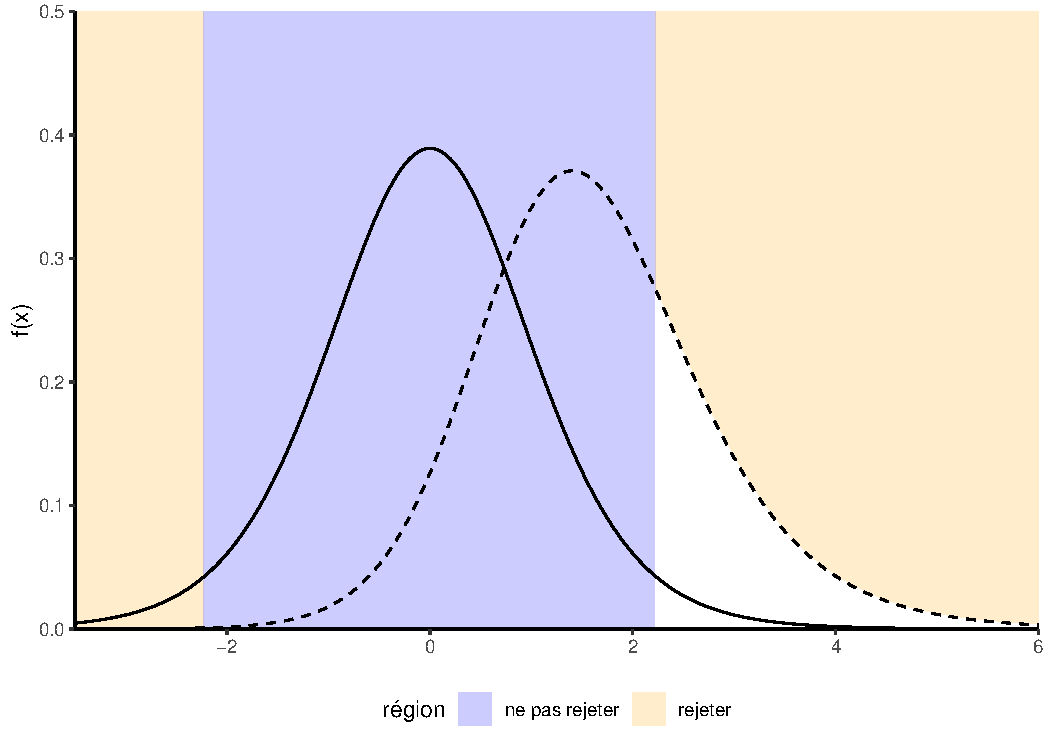
\includegraphics[width=0.7\linewidth]{MATH60604_Modelisation_statistique_files/figure-latex/puissance1-1} 

}

\caption{Comparaison de la loi nulle (ligne pleine) et d'une alternative spécifique pour un test-$t$ (ligne traitillée). La puissance correspond à l'aire sous la courbe de la densité de la loi alternative qui est dans la zone de rejet du test (en blanc).}\label{fig:puissance1}
\end{figure}

\begin{figure}

{\centering 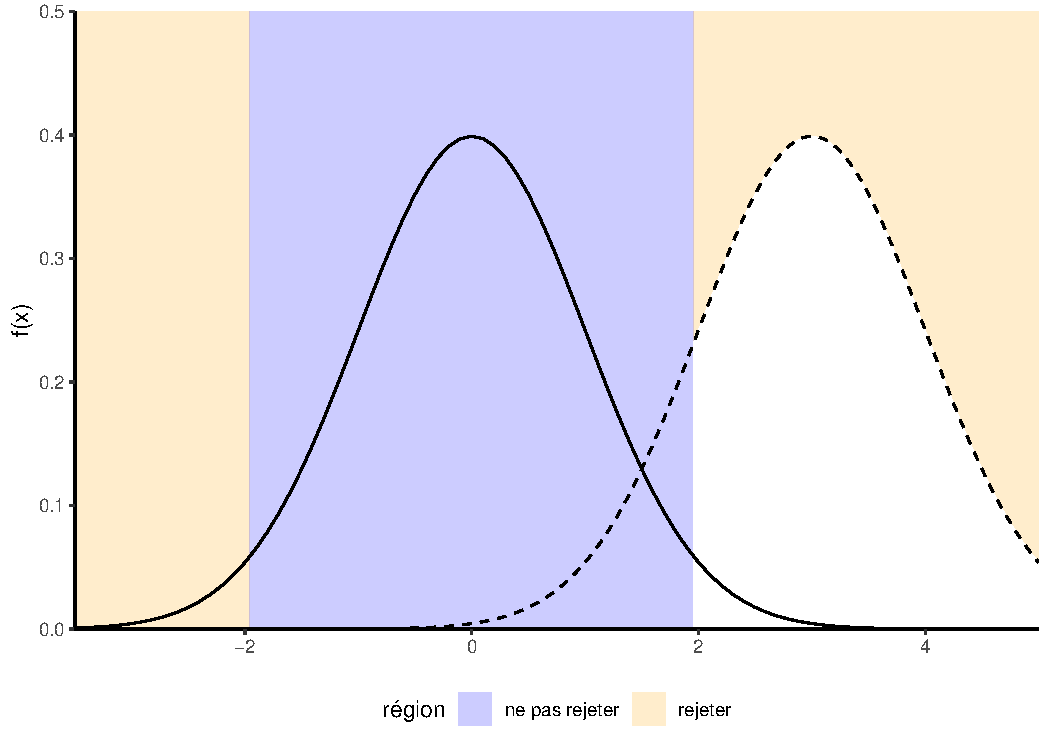
\includegraphics[width=0.7\linewidth]{MATH60604_Modelisation_statistique_files/figure-latex/puissance2-1} 

}

\caption{Augmentation de la puissance suite à une augmentation de la différence de moyenne sous l'hypothèse alternative. La puissance est l'aire sous la courbe (blanc) de la loi alternative (ligne traitillée); cette dernière est plus décalée vers la droite par rapport à la loi nulle postulée (ligne pleine).}\label{fig:puissance2}
\end{figure}

\begin{figure}

{\centering 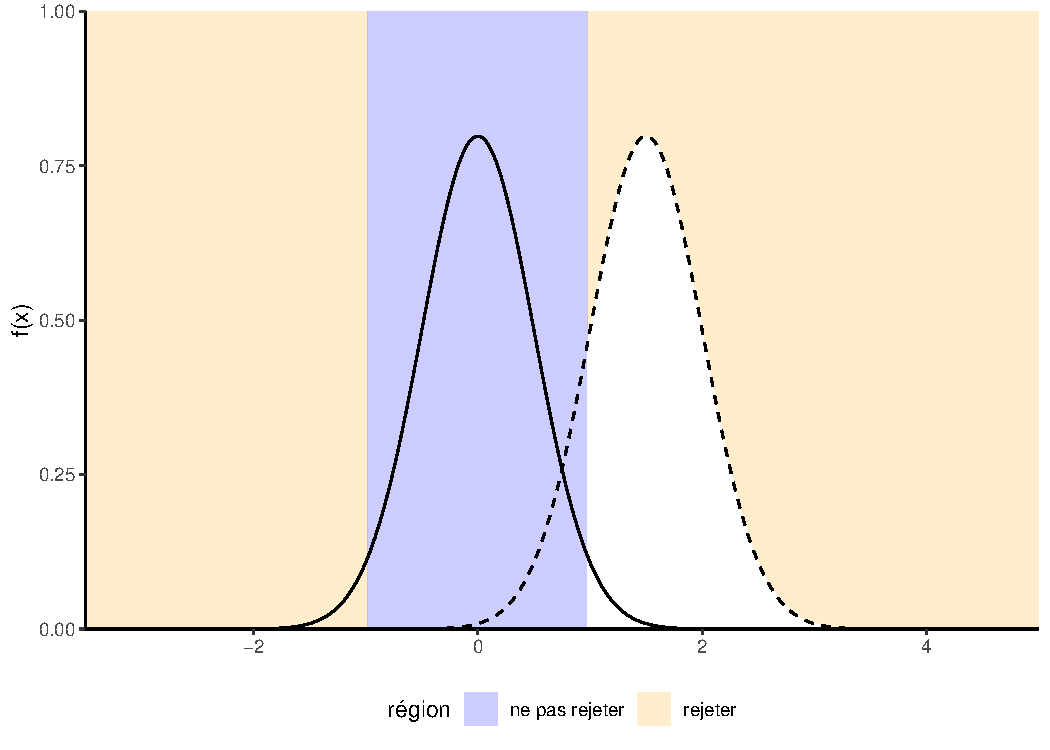
\includegraphics[width=0.7\linewidth]{MATH60604_Modelisation_statistique_files/figure-latex/puissance3-1} 

}

\caption{Augmentation de la puissance suite à une augmentation de la taille de l'échantillon ou une diminution de l'écart-type de la population: la loi nulle (ligne pleine) est plus concentrée et la taille de la région de rejet diminue. La puissance est l'aire sous la courbe (blanc) de la loi alternative (ligne traitillée). Règle générale, la loi nulle change selon la taille de l'échantillon.}\label{fig:puissance3}
\end{figure}

On veut qu'un test ait une puissance élevée, c'est-à-dire, on veut que \(\gamma\) soit le plus près de 1 possible. Minimalement, la puissance du test devrait être \(\alpha\) si on rejette l'hypothèse nulle une fraction \(\alpha\) du temps quand cette dernière est vraie. La puissance dépend de plusieurs critères, à savoir:

\begin{itemize}
\tightlist
\item
  la taille de l'effet: plus la différence est grande entre la valeur du paramètre postulé \(\theta_0\) sous \(\mathscr{H}_0\) et le comportement observé, plus il est facile de le détecter (voir Figure \ref{fig:puissance3});
\item
  la variabilité: moins les observations sont variables, plus il est facile de déterminer que la différence observée est significative (les grandes différences sont alors moins plausibles, comme l'illustre la Figure \ref{fig:puissance2});
\item
  la taille de l'échantillon: plus on a d'observations, plus notre capacité à détecter une différence significative augmente parce que l'erreur-type décroît avec la taille de l'échantillon à un rythme (ordinairement) de \(n^{-1/2}\). La loi nulle devient aussi plus concentrée quand la taille de l'échantillon augmente.
\item
  le choix de la statistique de test: par exemple, les statistiques basées sur les rangs n'utilisent pas les valeurs numériques qu'à travers le rang relatif. Ces tests sont donc moins puissants parce qu'ils n'utilisent pas toute l'information dans l'échantillon; en contrepartie, ils sont souvent plus robustes en présence de valeurs aberrantes et si le modèle est mal spécifié. Les statistiques de test que nous choisirons sont souvent standards et parmi les plus puissantes qui soient, aussi on ne traitera pas de ce point davantage dans le cadre du cours.
\end{itemize}

Pour calculer la puissance d'un test, il faut choisir une alternative spécifique. Pour des exemples simples de statistiques, on peut obtenir une formule pour la puissance: par exemple, si on utilise un test-\(t\) pour un échantillon, la statistique \(T=\sqrt{n}(\overline{X}-\mu_0)/S_n \sim \mathcal{T}_{n-1}\) et, si la vraie moyenne est \(\Delta + \mu_0\), alors la loi alternative est Student-\(t\), mais non-centrée avec paramètre de décalage \(\Delta\). Cette dérivation est l'exception plutôt que la règle et on détermine d'ordinaire la puissance à l'aide de méthodes de Monte Carlo en simulant des observations d'une alternative donnée, en calculant la statistique de test sur le nouvel échantillon simulé et en calculant la valeur-\emph{p} associée à notre hypothèse nulle de façon répétée. On calcule par la suite la proportion de tests qui mènent au rejet de l'hypothèse nulle à niveau \(\alpha\), ce qui correspond au pourcentage de valeurs-\(p\) inférieures à \(\alpha\).

\hypertarget{intervalle-de-confiance}{%
\subsubsection{Intervalle de confiance}\label{intervalle-de-confiance}}

Un \textbf{intervalle de confiance} est une manière alternative de rapporter les conclusions d'un test, en ce sens qu'on fournit une estimation ponctuelle de \(\hat{\theta}\) avec une marge d'erreur. L'intervalle de confiance donne donc une indication de la variabilité de la procédure d'estimation. Un intervalle de confiance de Wald à \((1-\alpha)\) pour un paramètre \(\theta\) est de la forme
\begin{align*}
\widehat{\theta} \pm \mathfrak{q}_{\alpha/2} \; \mathrm{se}(\widehat{\theta})
\end{align*}
où \(\mathfrak{q}_{\alpha/2}\) est le quantile d'ordre \(1-\alpha/2\) de la loi nulle de la statistique de Wald,
\begin{align*}
T =\frac{\widehat{\theta}-\theta}{\mathrm{se}(\widehat{\theta})},
\end{align*}
et où \(\theta\) représente la valeur du paramètre \(\theta\) (supposé fixe, mais inconnu) de la population. Les bornes de l'intervalle de confiance sont aléatoires puisque \(\widehat{\theta}\) et \(\mathrm{se}(\widehat{\theta})\) sont des variable aléatoires: leurs valeurs observées changent d'un échantillon à un autre.

Par exemple, pour un échantillon aléatoire \(X_1, \ldots, X_n\) provenant d'une loi normale \(\mathsf{No}(\mu, \sigma)\), l'intervalle de confiance à \((1-\alpha)\) pour la moyenne (dans la population) \(\mu\) est
\begin{align*}
\overline{X} \pm t_{n-1, \alpha/2} \frac{S}{\sqrt{n}}
\end{align*}
où \(t_{n-1, \alpha/2}\) est le quantile d'ordre \(1-\alpha/2\) de la loi Student-\(t\) avec \(n-1\) degrés de libertés.

Avant qu'on calcule l'intervalle de confiance, il y a une probabilité de \(1-\alpha\) que \(\theta\) soit contenu dans l'intervalle \textbf{aléatoire} symmétrique \((\widehat{\theta} - \mathfrak{q}_{\alpha/2} \; \mathrm{se}(\widehat{\theta}), \widehat{\theta} + \mathfrak{q}_{\alpha/2} \; \mathrm{se}(\widehat{\theta}))\), où \(\widehat{\theta}\) dénote l'estimateur de \(\theta\). Une fois qu'on obtient un échantillon et qu'on calcule les bornes de l'intervalle de confiance, il n'y a plus de notion de probabilité: la vraie valeur du paramètre \(\theta\) (inconnue) est soit contenue dans l'intervalle de confiance, soit pas. La seule interprétation de l'intervalle de confiance qui soit valable alors est la suivante: si on répète l'expérience plusieurs fois et qu'à chaque fois on calcule un intervalle de confiance à \(1-\alpha\), alors une proportion de \((1-\alpha)\) de ces intervalles devraient contenir la vraie valeur de \(\theta\) (de la même manière, si vous lancez une pièce de monnaie équilibrée, vous devriez obtenir grosso modo une fréquence de 50\% de pile et 50\% de face, mais chaque lancer donnera un ou l'autre de ces choix). Notre « confiance » est dans la procédure et non pas dans les valeurs numériques obtenues pour un échantillon donné.

\begin{figure}

{\centering 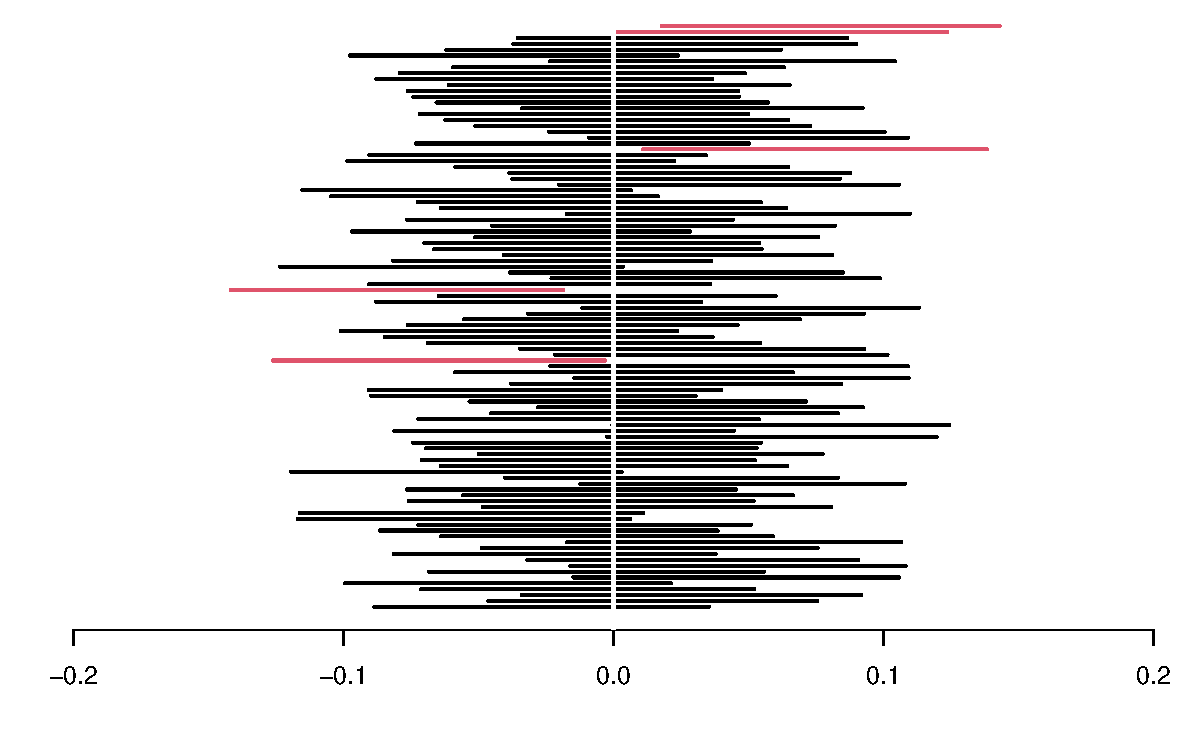
\includegraphics[width=0.7\linewidth]{MATH60604_Modelisation_statistique_files/figure-latex/intconf-1} 

}

\caption{Intervalles de confiance à 95\% pour la moyenne d'une population normale $\mathsf{No}(0,1)$ pour 100 échantillons aléatoires. En moyenne, 5\% de ces intervalles (en rouge) n'incluent pas la vraie valeur de la moyenne de zéro.}\label{fig:intconf}
\end{figure}

Si on s'intéresse seulement à la décision rejeter/ne pas rejeter \(\mathscr{H}_0\), l'intervalle de confiance est équivalent à la valeur-\emph{p} en ce sens qu'il mène à la même décision. L'intervalle de confiance donne en revanche l'ensemble des valeurs pour lesquelles la statistique de test ne fournit pas assez de preuves pour rejeter \(\mathscr{H}_0\): pour un test à niveau \(\alpha\), on ne rejetterait aucune des valeurs contenues dans l'intervalle de confiance de niveau \(1-\alpha\). Si la valeur-\emph{p} est inférieure à \(\alpha\), la valeur postulée pour \(\theta\) est donc hors de l'intervalle de confiance calculé. À l'inverse, la valeur-\emph{p} ne donne la probabilité d'obtenir un résultat aussi extrême sous l'hypothèse nulle que pour une seule valeur numérique, mais permet de quantifier précisément à quel point le résultat est extrême.

\begin{example}[Achat en ligne de milléniaux]
\protect\hypertarget{exm:achats-milleniaux}{}{\label{exm:achats-milleniaux} \iffalse (Achat en ligne de milléniaux) \fi{} }
Supposons qu'une chercheuse veut faire une étude sur l'évolution des ventes en ligne au Canada. Elle postule que les membres de la génération Y fait plus d'achats en ligne que ceux des générations antérieures. Pour répondre à cette question, un sondage est envoyé à un échantillon aléatoire de \(n=500\) individus représentatif de la population avec 160 membres de la génération Y et 340 personnes plus âgées. La variable réponse est le montant d'achat effectués en ligne dans le mois dernier (en dollars).
\end{example}

Dans cet exemple, on s'intéresse à la différence entre le montant moyen des Y et celui des générations antérieures: la différence de moyenne observée dans l'échantillon est de 16.49 dollars et donc les milléniaux ont dépensé davantage. En revanche, notre échantillon est aléatoire et le montant d'achat en ligne varie d'un individu à l'autre (et d'un mois à l'autre): ce n'est donc pas suffisant pour dire que la différence est significative.

La première étape de notre analyse consiste à définir les quantités d'intérêt et à formuler nos hypothèse en fonction de paramètres du modèle; il convient également de définir ces derniers en fonction des variables en présence dans l'exemple. Ici, on considère un test pour la différence de moyenne dans les populations postulées \(\mu_1\) (pour la génération Y) et \(\mu_2\) (pour les générations antérieures) d'écart-type respectif \(\sigma_1\) et \(\sigma_2\). Comment déterminer quelle hypothèse on considère? Comme statisticien, on se fait l'avocat du Diable: l'hypothèse d'intérêt du chercheur est l'hypothèse alternative et ici, \(\mathscr{H}_a: \mu_1 > \mu_2\), où \(\mu_1\) représente la moyenne des achats mensuels des milléniaux. L'hypothèse nulle comprend toutes les autres valeurs pour la différence de moyenne, soit \(\mathscr{H}_0: \mu_1 \leq \mu_2\). Il suffit néanmoins de considérer le cas \(\mu_1=\mu_2\) (pourquoi?)

La deuxième étape consiste à choisir une statistique de test. S'il n'y a aucune différence de moyenne entre les groupes, alors \(\overline{X}_1-\overline{X}_2\) a moyenne zéro et la différence de moyenne a une variance de \(\sigma^2_1/n_1+\sigma^2_2/n_2\). Ici, on considère la statistique de \citet{Welch1947} pour une différence de moyenne entre deux échantillons:
\begin{align*}
T = \frac{\overline{X}_1 - \overline{X}_2}{\left(\frac{S_1^2}{n_1}+\frac{S_2^2}{n_2} \right)^{1/2}}, \end{align*}
où \(\overline{X}_i\) est la moyenne empirique dans l'échantillon \(i\) (\(i=1, 2\)) et \(S_i^2\) est la variance empirique et \(n_i\) la taille de l'échantillon du groupe \(i\). La statistique est utilisée pour calculer la différence de moyennes de deux échantillons de variance potentiellement différente. La valeur de la statistique dans l'échantillon est \(T=2.76\), mais on obtiendrait une valeur différente avec un autre échantillon. Il convient donc de déterminer si cette valeur est compatible avec notre hypothèse nulle en la comparant à la loi nulle sous \(\mathscr{H}_0\) de \(T\). On effectuera le test à niveau \(\alpha=0.05\).

La troisième étape est l'obtention d'un étalon de mesure pour déterminer si notre résultat est extrême ou inattendu. Vous remarquerez que la statistique de Welch a moyenne zéro et variance un sous l'hypothèse nulle que \(\mu_1=\mu_2\): standardiser une statistique permet d'obtenir un objet dont on connaît le comportement pour de grands échantillons et obtenir une quantité sans unité de mesure. La dérivation de la loi nulle est hors objectifs du cours, aussi cette dernière vous sera donnée dans tous les cas qu'on considère. Asymptotiquement, \(T\) suit une loi normale \(\mathsf{No}(0, 1)\), mais il existe une meilleure approximation pour \(n\) petit; on compare le comportement de \(T\) à l'aide d'une loi de Student (à l'aide de l'approximation de \citet{Satterthwaite1946}).

La dernière étape consiste à obtenir une valeur-\emph{p}, soit la probabilité d'observer un résultat aussi extrême sous \(\mathscr{H}_0\): l'avantage de la valeur-\emph{p} est que cette valeur est une probabilité (dans \([0, 1]\)) et qu'elle suit une loi uniforme sous \(\mathscr{H}_0\). Puisque nous avons une hypothèse alternative unilatérale, on regarde la probabilité sous \(\mathscr{H}_0\) que \(\mathsf{Pr}(T > t)\). La valeur-\emph{p} vaut \(0.0031\) et donc, à niveau 5\%, on rejette l'hypothèse nulle pour conclure que la génération Y dépense davantage en ligne que les générations antérieures.

\begin{example}[Prix de billets de trains à grande vitesse espagnols]
\protect\hypertarget{exm:prix-trains-tests}{}{\label{exm:prix-trains-tests} \iffalse (Prix de billets de trains à grande vitesse espagnols) \fi{} }La compagnie nationale de chemin de fer \href{https://www.renfe.com/}{Renfe} gère les trains régionaux et les trains à haute vitesse dans toute l'Espagne. Les prix des billets vendus par Renfe sont \href{https://www.kaggle.com/thegurusteam/spanish-high-speed-rail-system-ticket-pricing}{aggrégés} par une compagnie. On s'intéresse ici à une seule ligne, Madrid--Barcelone. Notre question scientifique est la suivante: est-ce que le prix des billets pour un aller (une direction) est plus chère pour un retour? Pour ce faire, on considère un échantillon de 10000 billets entre les deux plus grandes villes espagnoles. On s'intéresse au billets de TGV vendus (AVE) au tarif Promotionnel. Notre statistique de test sera simplement la différence de moyenne entre les deux échantillons: la différence entre le prix en euros d'un train Madrid--Barcelone (\(\mu_1\)) et le prix d'un billet Barcelone--Madrid (\(\mu_2\)) est \(\mu_1-\mu_2\) et notre hypothèse nulle est qu'il n'y a aucune différence de prix, soit \(\mathscr{H}_0: \mu_1-\mu_2=0\). On utilise de nouveau le test de Welch pour deux échantillons.
\end{example}

\begin{Shaded}
\begin{Highlighting}[]
\CommentTok{\# Manipulation de données, incluant \%\textgreater{}\%}
\FunctionTok{library}\NormalTok{(poorman)}
\CommentTok{\# Charger les données}
\FunctionTok{data}\NormalTok{(renfe, }\AttributeTok{package =} \StringTok{"hecmodstat"}\NormalTok{)}
\FunctionTok{head}\NormalTok{(renfe, }\AttributeTok{n =} \DecValTok{5}\NormalTok{)}
\end{Highlighting}
\end{Shaded}

\begin{verbatim}
## # A tibble: 5 x 7
##    prix type    classe     tarif    dest             duree jour 
##   <dbl> <fct>   <fct>      <fct>    <fct>            <dbl> <fct>
## 1 143.  AVE     Preferente Promo    Barcelone-Madrid   190 6    
## 2 182.  AVE     Preferente Flexible Barcelone-Madrid   190 2    
## 3  86.8 AVE     Preferente Promo    Barcelone-Madrid   165 7    
## 4  86.8 AVE     Preferente Promo    Barcelone-Madrid   190 7    
## 5  69.0 AVE-TGV Preferente Promo    Barcelone-Madrid   175 4
\end{verbatim}

\begin{Shaded}
\begin{Highlighting}[]
\CommentTok{\# Sous{-}échantillon avec uniquement les données au tarif promotionnel}
\NormalTok{renfe\_promo }\OtherTok{\textless{}{-}}\NormalTok{ renfe }\SpecialCharTok{\%\textgreater{}\%} \FunctionTok{subset}\NormalTok{(tarif }\SpecialCharTok{==} \StringTok{"Promo"}\NormalTok{)}
\CommentTok{\# Test{-}t et différence de moyenne}
\NormalTok{ttest }\OtherTok{\textless{}{-}} \FunctionTok{t.test}\NormalTok{(prix}\SpecialCharTok{\textasciitilde{}}\NormalTok{dest, }\AttributeTok{data =}\NormalTok{ renfe\_promo)}
\NormalTok{ttest }\CommentTok{\#imprimer le résultat}
\end{Highlighting}
\end{Shaded}

\begin{verbatim}
## 
##  Welch Two Sample t-test
## 
## data:  prix by dest
## t = -1, df = 8040, p-value = 0.2
## alternative hypothesis: true difference in means is not equal to 0
## 95 percent confidence interval:
##  -1.100  0.209
## sample estimates:
## mean in group Barcelone-Madrid mean in group Madrid-Barcelone 
##                           82.1                           82.6
\end{verbatim}

Plutôt que d'utiliser la loi asymptotique (qui est valide pour de grands échantillons à cause du théorème central limite), on peut considérer une approximation sous une hypothèse moins restrictive en supposant que les données sont échangeables. Sous l'hypothèse nulle, il n'y aucune différence entre les deux destinations et les étiquettes pour la destination (une variable catégorielle binaire) sont arbitraires. On pourrait considérer les mêmes données, mais avec une permutation des variables explicatives: c'est ce qu'on appelle un \href{https://www.jwilber.me/permutationtest/}{test de permutation}. On va recréer deux groupes de taille identique à notre échantillon original, mais en changeant les observations. On recalcule la statistique de test sur ces nouvelle données (si on a une poignée d'observations, il est possible de lister toutes les permutations possibles; typiquement, il suffit de considérer un grand nombre de telles permutations, disons 9999). Pour chaque nouveau jeu de données, on calculera la statistique de test et on calculera le rang de notre statistique par rapport à cette référence. Si la valeur de notre statistique observée sur l'échantillon original est extrême en comparaison, c'est autant de preuves contre l'hypothèse nulle.

\begin{Shaded}
\begin{Highlighting}[]
\CommentTok{\# Valeur{-}p par permutation}
\NormalTok{n }\OtherTok{\textless{}{-}} \FunctionTok{nrow}\NormalTok{(renfe\_promo)}
\NormalTok{B }\OtherTok{\textless{}{-}} \FloatTok{1e4}
\NormalTok{ttest\_stats }\OtherTok{\textless{}{-}} \FunctionTok{numeric}\NormalTok{(B) }
\NormalTok{ttest\_stats[}\DecValTok{1}\NormalTok{] }\OtherTok{\textless{}{-}}\NormalTok{ ttest}\SpecialCharTok{$}\NormalTok{statistic}
\FunctionTok{set.seed}\NormalTok{(}\DecValTok{20200608}\NormalTok{) }\CommentTok{\# germe pour nombres pseudo{-}aléatoires}
\ControlFlowTok{for}\NormalTok{(i }\ControlFlowTok{in} \DecValTok{2}\SpecialCharTok{:}\NormalTok{B)\{}
  \CommentTok{\# Recalculer la statistique de test, mais permuter les étiquettes}
\NormalTok{  ttest\_stats[i] }\OtherTok{\textless{}{-}} \FunctionTok{t.test}\NormalTok{(prix }\SpecialCharTok{\textasciitilde{}}\NormalTok{ dest[}\FunctionTok{sample.int}\NormalTok{(}\AttributeTok{n =}\NormalTok{ n)], }
                           \AttributeTok{data =}\NormalTok{ renfe\_promo)}\SpecialCharTok{$}\NormalTok{statistic}
\NormalTok{\}}
\CommentTok{\# Bibliothèque graphique}
\FunctionTok{library}\NormalTok{(ggplot2)}
\CommentTok{\# Tracer un graphique de la distribution empirique obtenue par permutation}
\FunctionTok{ggplot}\NormalTok{(}\AttributeTok{data =} \FunctionTok{data.frame}\NormalTok{(}\AttributeTok{statistique =}\NormalTok{ ttest\_stats), }
       \FunctionTok{aes}\NormalTok{(}\AttributeTok{x=}\NormalTok{statistique)) }\SpecialCharTok{+}
  \FunctionTok{geom\_histogram}\NormalTok{(}\AttributeTok{bins =} \DecValTok{30}\NormalTok{, }\FunctionTok{aes}\NormalTok{(}\AttributeTok{y=}\NormalTok{..density..), }\AttributeTok{alpha =} \FloatTok{0.2}\NormalTok{) }\SpecialCharTok{+} 
  \FunctionTok{geom\_density}\NormalTok{() }\SpecialCharTok{+} 
  \FunctionTok{geom\_vline}\NormalTok{(}\AttributeTok{xintercept =}\NormalTok{ ttest\_stats[}\DecValTok{1}\NormalTok{]) }\SpecialCharTok{+} 
  \FunctionTok{ylab}\NormalTok{(}\StringTok{"densité"}\NormalTok{) }\SpecialCharTok{+} 
  \FunctionTok{stat\_function}\NormalTok{(}\AttributeTok{fun =}\NormalTok{ dnorm, }\AttributeTok{col =} \StringTok{"blue"}\NormalTok{)}
\end{Highlighting}
\end{Shaded}

\begin{figure}

{\centering 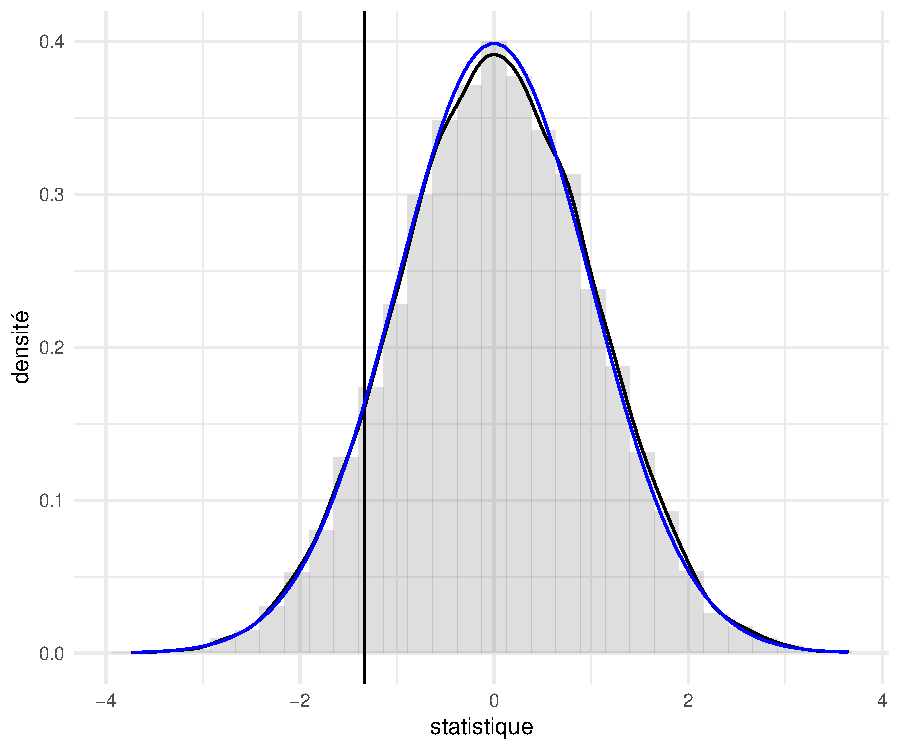
\includegraphics[width=0.7\linewidth]{MATH60604_Modelisation_statistique_files/figure-latex/renfepermut-1} 

}

\caption{Approximation par permutation de la loi nulle de la statistique de test de Welch (histogramme et trait noir) et loi asymptotique normale standard (trait bleu) pour le prix de billets de trains AVE au tarif promotionnel entre Madrid et Barcelone. La valeur de la statistique de test de l'échantillon original est représentée par un trait vertical.}\label{fig:renfepermut}
\end{figure}

La valeur-\emph{p} du test de permutation, \(0.186\), est la proportion de statistiques plus extrêmes que celle observée. Cette valeur-\emph{p} est quasi-identique à celle de l'approximation de Satterthwaite, à savoir \(0.182\) (la loi Student-\(t\) est numériquement équivalente à une loi standard normale avec autant de degrés de liberté), tel que représenté dans la Figure \ref{fig:renfepermut}. Malgré que notre échantillon soit très grand, avec \(n=8059\) observations, la différence n'est pas jugée significative. Avec un échantillon de deux millions de billets, on pourrait estimer précisément la moyenne (au centime près): la différence de prix entre les deux destinations et cette dernière deviendrait statistiquement significative. Elle n'est pas en revanche pertinente (une différence de \(0.28\) euros sur un prix moyen de \(82.56\) euros est quantité négligeable).

\hypertarget{analyse-exploratoire}{%
\subsection{Analyse exploratoire de données}\label{analyse-exploratoire}}

L'analyse exploratoire, comme son nom l'indique, est une étape préliminaire à la modélisation servant à l'acquisition d'une meilleure compréhension des données.
Une connaissance rudimentaire des graphiques est nécessaire et on s'attardera aux \href{https://rstudio.cloud/learn/primers/1.1}{rudiments de la visualisation graphique}. Plusieurs ouvrages abordent ces notions (en anglais) .

\begin{itemize}
\tightlist
\item
  \href{https://r4ds.had.co.nz/exploratory-data-analysis.html}{Chapitre 3 de \emph{\textbf{R} for Data Science} par Garrett Grolemund et Hadley Wickham}
\item
  \href{https://www.openintro.org/book/isrs/}{Section 1.6 du livre \emph{Introductory Statistics with Randomization and Simulation} d'OpenIntro}
\item
  \href{https://clauswilke.com/dataviz/}{\emph{Fundamentals of Data Visualization} par Claus O. Wilke}
\item
  \href{https://socviz.co/lookatdata.html\#lookatdata}{Chapitre 1 de \emph{Data Visualization: A practical introduction} par Kieran Healy}
\end{itemize}

Si l'analyse exploratoire est souvent négligée dans les cours de statistique (parce qu'elle n'a pas de fondement mathématique), elle n'en est pas moins importante car elle nous sert à interpréter les données dans le contexte du problème et à nous assurer que notre analyse ou notre traitement de ces dernières est cohérent. Le sujet est difficile à cerner, puisque c'est davantage un art qu'une approche rigoureuse; Grolemund et Wickham parlent même « d'état d'esprit ». Le but de l'analyse exploratoire graphique est d'extraire des informations utiles, le plus souvent par le biais d'une série de questions qui sont raffinées au fur et à mesure que progresse l'analyse. On s'intéresse particulièrement aux relations et interactions entre différentes variables et la distribution empirique de chaque variable. Les étapes majeures sont:

\begin{enumerate}
\def\labelenumi{\arabic{enumi}.}
\tightlist
\item
  Formuler des questions sur les données
\item
  Chercher des réponses à ces questions à l'aide de statistiques descriptives, de tableaux de fréquence ou de contingence et de graphiques.
\item
  Raffiner nos questions, et utiliser les trouvailles pour peaufiner notre analyse
\end{enumerate}

Dans un rapport, un résumé des caractéristiques les plus importantes devrait être inclut pour que le lecteur ou la lectrice puisse valider son interprétation des données.

\hypertarget{soignez-votre-travail}{%
\subsubsection{Soignez votre travail}\label{soignez-votre-travail}}

Si vous incluez un graphique (ou un tableau), il est important d'ajouter une légende qui décrit le graphique et le résume, les noms de variables (avec les unités) sur les axes, mais aussi de soigner le rendu et le formatage pour obtenir un produit fini propre, lisible et cohérent: en particulier, votre description devrait coïncider avec le rendu. Votre graphique raconte une histoire, aussi prenez-soin que cette dernière soit nécessaire et attrayante.

\hypertarget{types-de-variables}{%
\subsubsection{Types de variables}\label{types-de-variables}}

Commençons par parler des données: celles que l'on manipulera dans ce cours sont stockées sous forme tabulaire. Dans une base de donnée en format long, chaque ligne correspond à une observation et chaque colonne à une variable; les entrées de la base de données contiennent les valeurs.

L'alternative au format long est le format court/large, où les colonnes représentent les modalités de variables catégorielles et il peut y avoir plusieurs valeurs par ligne qui contiennent des valeurs de la variable réponse. Le schéma de la Figure \ref{fig:longvswide} permet de mieux comprendre la distinction entre les deux formats: on supposera que nos données sont toujours en format long, ce dernier étant assumé par défaut par le logiciel pour procéder à l'ajustement d'un modèle..

\textbackslash begin\{figure\}

\{\centering 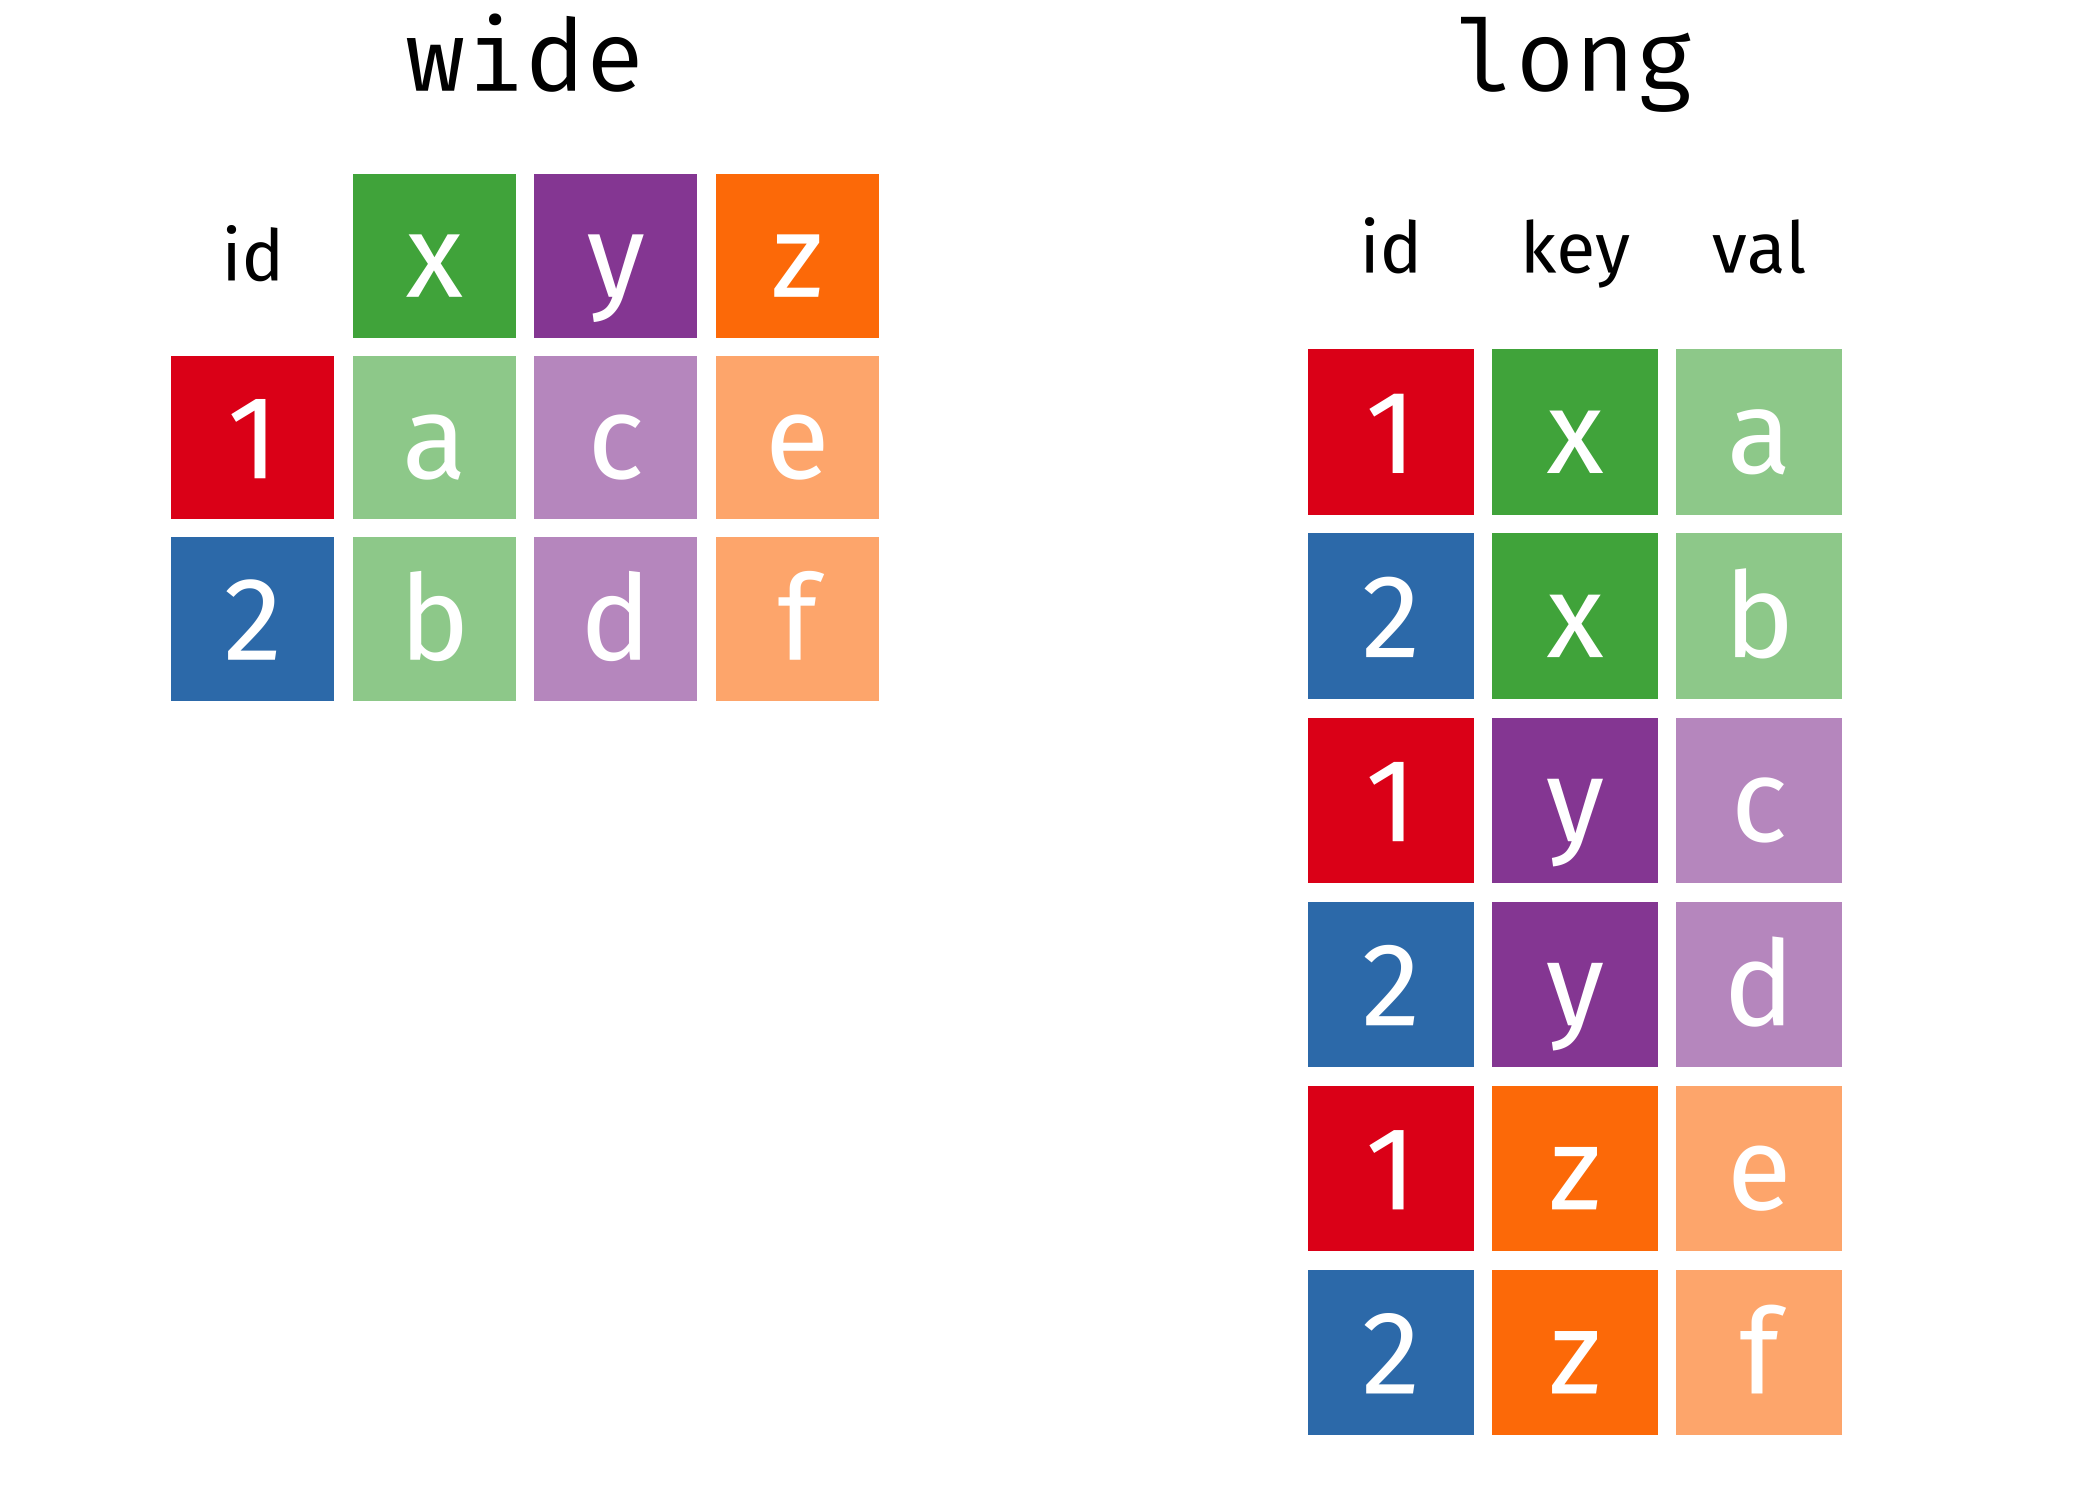
\includegraphics[width=0.7\linewidth]{images/original-dfs-tidy}

\}

\textbackslash caption\{Format long versus format large (\emph{wide}) (dessin de Garrick Aden-Buie).\}\label{fig:longvswide}
\textbackslash end\{figure\}

\begin{itemize}
\tightlist
\item
  Une \textbf{variable} représente une caractéristique de la population d'intérêt, par exemple le sexe d'un individu, le prix d'un article, etc.
\item
  une \textbf{observation}, parfois appelée donnée, est un ensemble de mesures collectées sous des conditions identiques, par exemple pour un individu ou à un instant donné.
\end{itemize}

Le choix de modèle statistique ou de test dépend souvent du type de variables collectées. Les variables peuvent être de plusieurs types: quantitatives (discrètes ou continues) si elles prennent des valeurs numériques, qualitatives (binaires, nominales ou ordinales) si elles sont décrites par un adjectif; je préfère le terme catégorielle, plus évocateur.

Les modèles de régression servent à expliquer des variables quantitatives en fonction d'autres caractéristiques.

\begin{itemize}
\tightlist
\item
  une variable discrète prend un nombre dénombrable de valeurs; ce sont souvent des variables de dénombrement ou des variables dichotomiques.
\item
  une variable continue peut prendre (en théorie) une infinité de valeurs, même si les valeurs mesurées sont arrondies ou mesurées avec une précision limitée (temps, taille, masse, vitesse, salaire). Dans bien des cas, nous pouvons considérer comme continues des variables discrètes si elles prennent un assez grand nombre de valeurs.
\end{itemize}

Les variables catégorielles représentent un ensemble fini de possibilités. On les regroupe en deux types, pour lesquels on ne fera pas de distinction: nominales s'il n'y a pas d'ordre entre les modalités (sexe, couleur, pays d'origine) ou ordinale (échelle de Likert, tranche salariale). La codification des modalités des variables catégorielle est arbitraire; en revanche, on préservera l'ordre lorsqu'on représentera graphiquement les variables ordinales. Lors de l'estimation, chaque variable catégorielle doit est transformée en un ensemble d'indicateurs binaires: il est donc essentiel de déclarer ces dernières dans votre logiciel statistique, surtout si elles sont parfois encodées dans la base de données à l'aide de valeurs entières.

\hypertarget{graphiques}{%
\subsubsection{Graphiques}\label{graphiques}}

Le principal type de graphique pour représenter la distribution d'une variable catégorielle est le diagramme en bâtons, dans lequel la fréquence de chaque catégorie est présentée sur l'axe des ordonnées (\(y\)) en fonction de la modalité, sur l'axe des abscisses (\(x\)), et ordonnées pour des variables ordinales. Cette représentation est en tout point supérieur au \href{http://www.perceptualedge.com/articles/08-21-07.pdf}{diagramme en camembert}, une engeance répandu qui devrait être honnie (notamment parce que l'humain juge mal les différences d'aires, qu'une simple rotation change la perception du graphique et qu'il est difficile de mesurer les proportions) --- ce n'est pas de la tarte!

\begin{figure}

{\centering 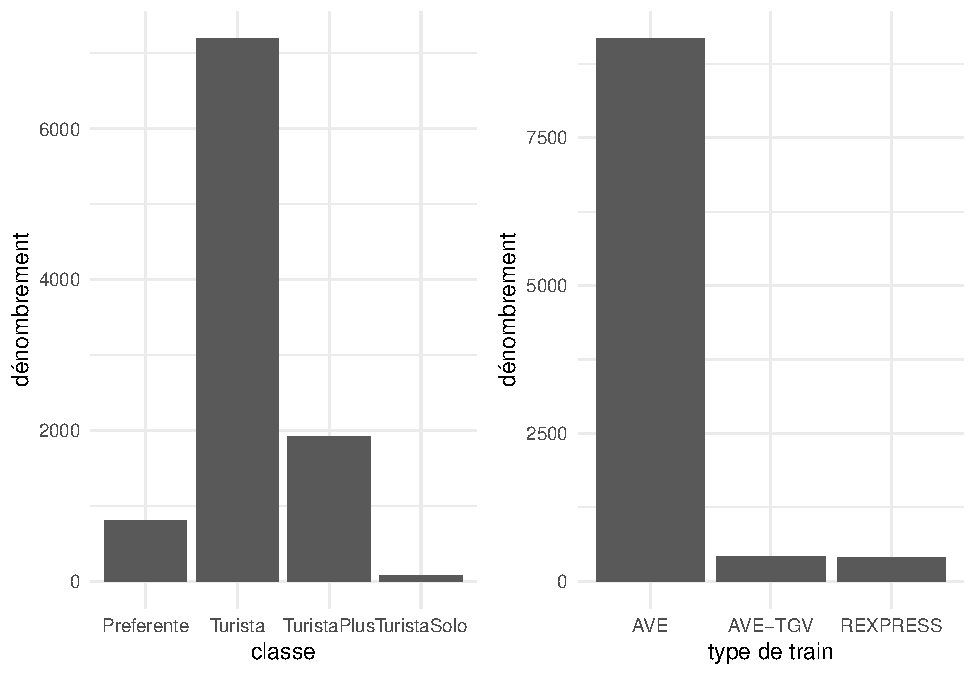
\includegraphics[width=0.7\linewidth]{MATH60604_Modelisation_statistique_files/figure-latex/barplotrenfe-1} 

}

\caption{Diagramme en bâtons pour la classe des billets de trains du jeu de données Renfe.}\label{fig:barplotrenfe}
\end{figure}

Puisque les variables continues peuvent prendre autant de valeurs distinctes qu'il y a d'observations, on ne peut simplement compter le nombre d'occurrence par valeur unique. On regroupera plutôt dans un certain nombre d'intervalle, en discrétisant l'ensemble des valeurs en classes pour obtenir un histogramme. Le nombre de classes dépendra du nombre d'observations si on veut que l'estimation ne soit pas impactée par le faible nombre d'observations par classe: règle générale, le nombre de classes ne devrait pas dépasser \(\sqrt{n}\), où \(n\) est le nombre d'observations de l'échantillon. On obtiendra la fréquence de chaque classe, mais si on normalise l'histogramme (de façon à ce que l'aire sous les bandes verticales égale un), on obtient une approximation discrète de la fonction de densité. Faire varier le nombre de classes permet parfois de faire apparaître des caractéristiques de la variable (notamment la multimodalité, l'asymmétrie et les arrondis).

Puisque qu'on groupe les observations en classe pour tracer l'histogramme, il est difficile de voir l'étendue des valeurs que prenne la variable: on peut rajouter des traits sous l'histogramme pour représenter les valeurs uniques prises par la variable, tandis que la hauteur de l'histogramme nous renseigne sur leur fréquence relative.

\begin{figure}

{\centering 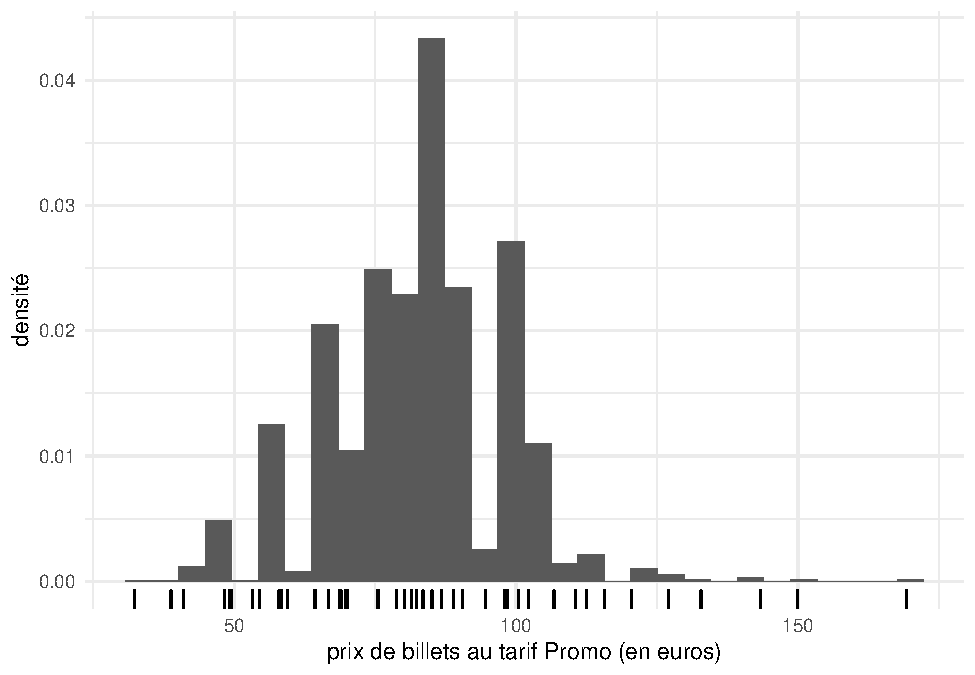
\includegraphics[width=0.7\linewidth]{MATH60604_Modelisation_statistique_files/figure-latex/histrenfe-1} 

}

\caption{Histogramme du prix des billets au tarif Promo de trains du jeu de données Renfe}\label{fig:histrenfe}
\end{figure}

Une boîte à moustaches(\emph{boxplot}) représente graphiquement cinq statistiques descriptives.

\begin{itemize}
\tightlist
\item
  La boîte donne les 1e, 2e et 3e quartiles \(q_1, q_2, q_3\). Il y a donc 50\% des observations sont au-dessus/en-dessous de la médiane \(q_2\) qui sépare en deux la boîte.
\item
  La longueur des moustaches est moins de \(1.5\) fois l'écart interquartile \(q_3-q_1\) (tracée entre 3e quartile et le dernier point plus petit que \(q_3+1.5(q_3-q_1)\), etc.)
\item
  Les observations au-delà des moustaches sont encerclées. Notez que plus le nombre d'observations est élevé, plus le nombres de valeurs aberrantes augmente. C'est un défaut de la boîte à moustache, qui a été conçue pour des jeux de données qui passeraient pour petits selon les standards actuels.
\end{itemize}

\begin{figure}

{\centering 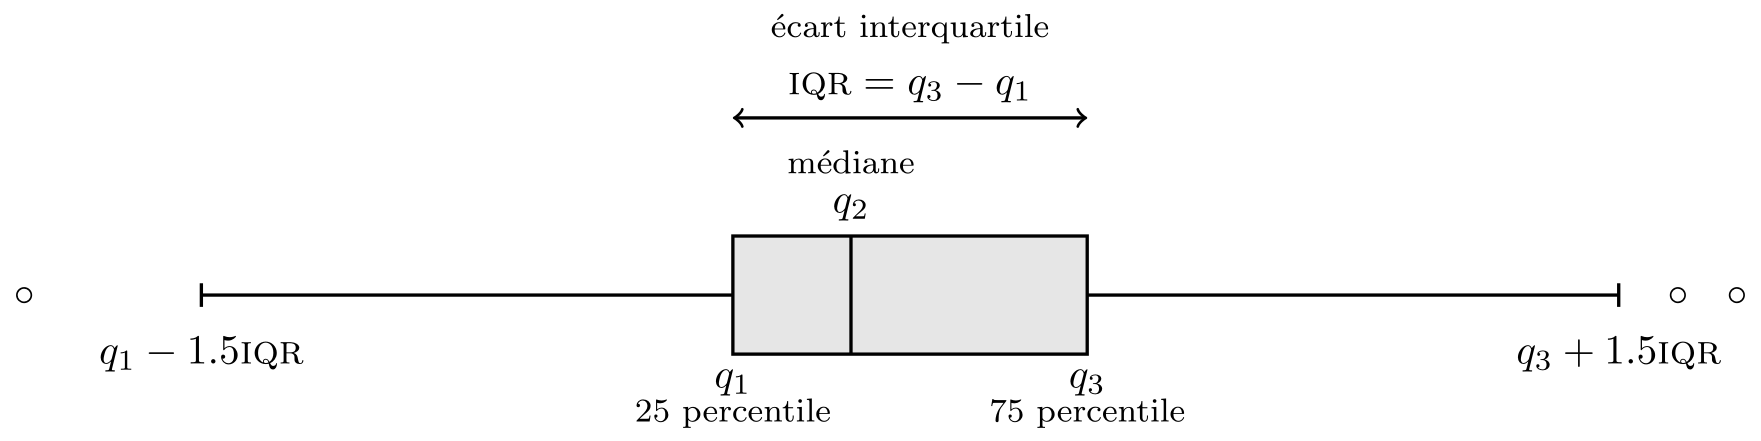
\includegraphics[width=0.7\linewidth]{images/01-intro-boiteamoustache} 

}

\caption{Boîte à moustache.}\label{fig:boiteamoustache}
\end{figure}

On peut représenter la distribution d'une variable réponse continue en fonction d'une variable catégorielle en traçant une boîte à moustaches pour chaque catégorie et en les disposant côte-à-côte. Une troisième variable catégorielle peut être ajoutée par le biais de couleurs, comme dans la Figure \ref{fig:histboxplot}.

\begin{figure}

{\centering 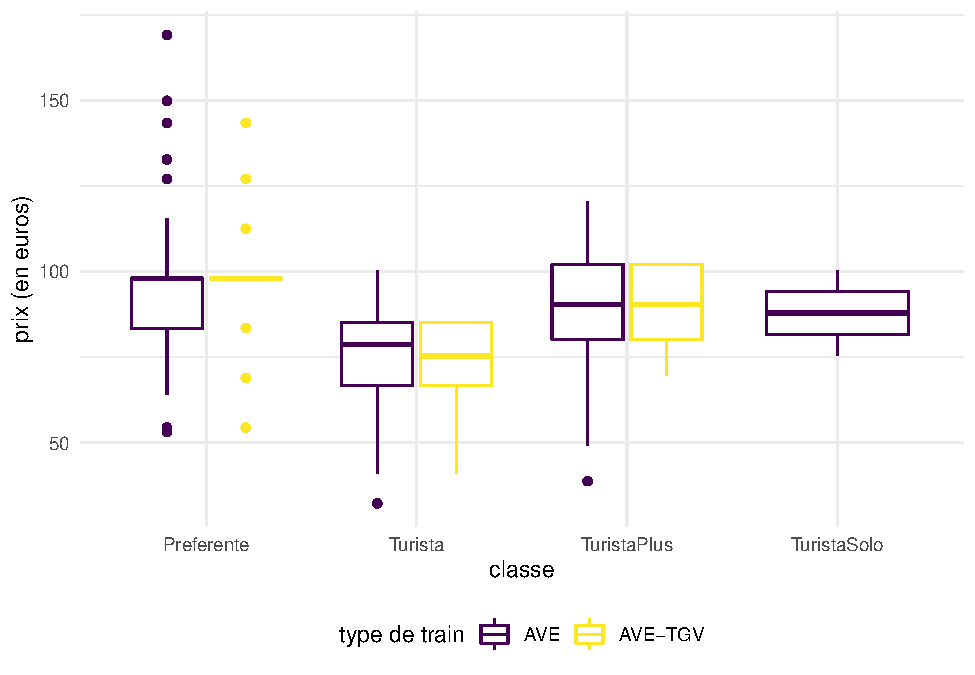
\includegraphics[width=0.7\linewidth]{MATH60604_Modelisation_statistique_files/figure-latex/histboxplot-1} 

}

\caption{Boîte à moustaches du prix des billets au tarif Promo en fonction de la classe pour le jeu de données Renfe.}\label{fig:histboxplot}
\end{figure}

Si on veut représenter la covariabilité de deux variables continues, on utilise un nuage de points où chaque variable est représentée sur un axe et chaque observation donne la coordonnée des points. Si la représentation graphique est dominée par quelques valeurs très grandes, une transformation des données peut être utile: vous verrez souvent des données positives à l'échelle logarithmique. Avec des données massives, les points seront superposés et le diagramme risque d'être illisible. Parmi les solutions envisagées, l'utilisation de la transparence, qui permet de voir où les points sont plus fréquents, ou encore un diagramme avec des classes hexagonale, l'équivalent d'un histogramme bidimensionnel où on remplace les classes par des hexagones. Le panneau de gauche de la Figure \ref{fig:nuagedepoints} représente ainsi 100 observations simulées à l'aide d'un nuage de points 100 observations, tandis simulées. Dans le panneau de droite, on utilise plutôt un diagramme hexagonal pour représenter les 10 000 points, ce qui donne un aperçu de la densité conjointe des deux variables.

\begin{figure}

{\centering 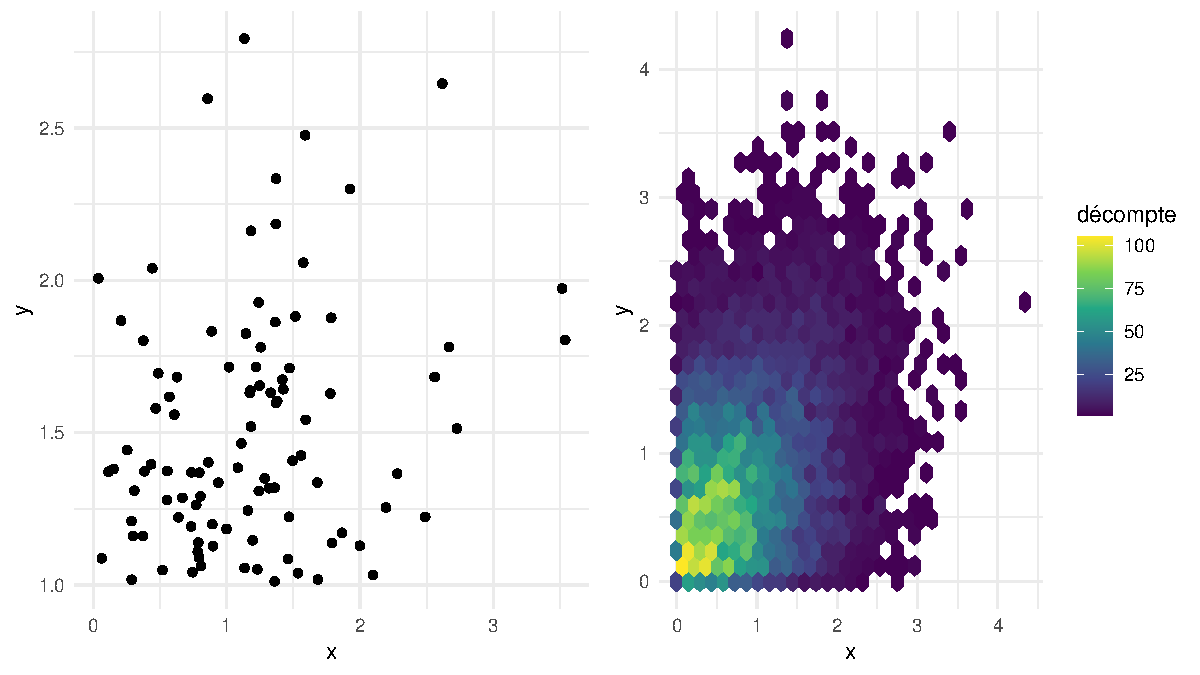
\includegraphics[width=0.7\linewidth]{MATH60604_Modelisation_statistique_files/figure-latex/nuagedepoints-1} 

}

\caption{Nuage de points (gauche) et diagramme hexagonal (droite) pour des données simulées.}\label{fig:nuagedepoints}
\end{figure}

Certaines données ont une structure particulière: pensons aux séries chronologiques, aussi appelées séries temporelles, qui comportent des observations ordonnées dans le temps. On représente chaque variable d'une série chronologique (sur l'axe des \(y\)) en fonction du temps (sur l'axe des \(x\)). Il est d'usage de relier les observations, bien que cet aperçu soit parfois trompeur.

\begin{figure}

{\centering 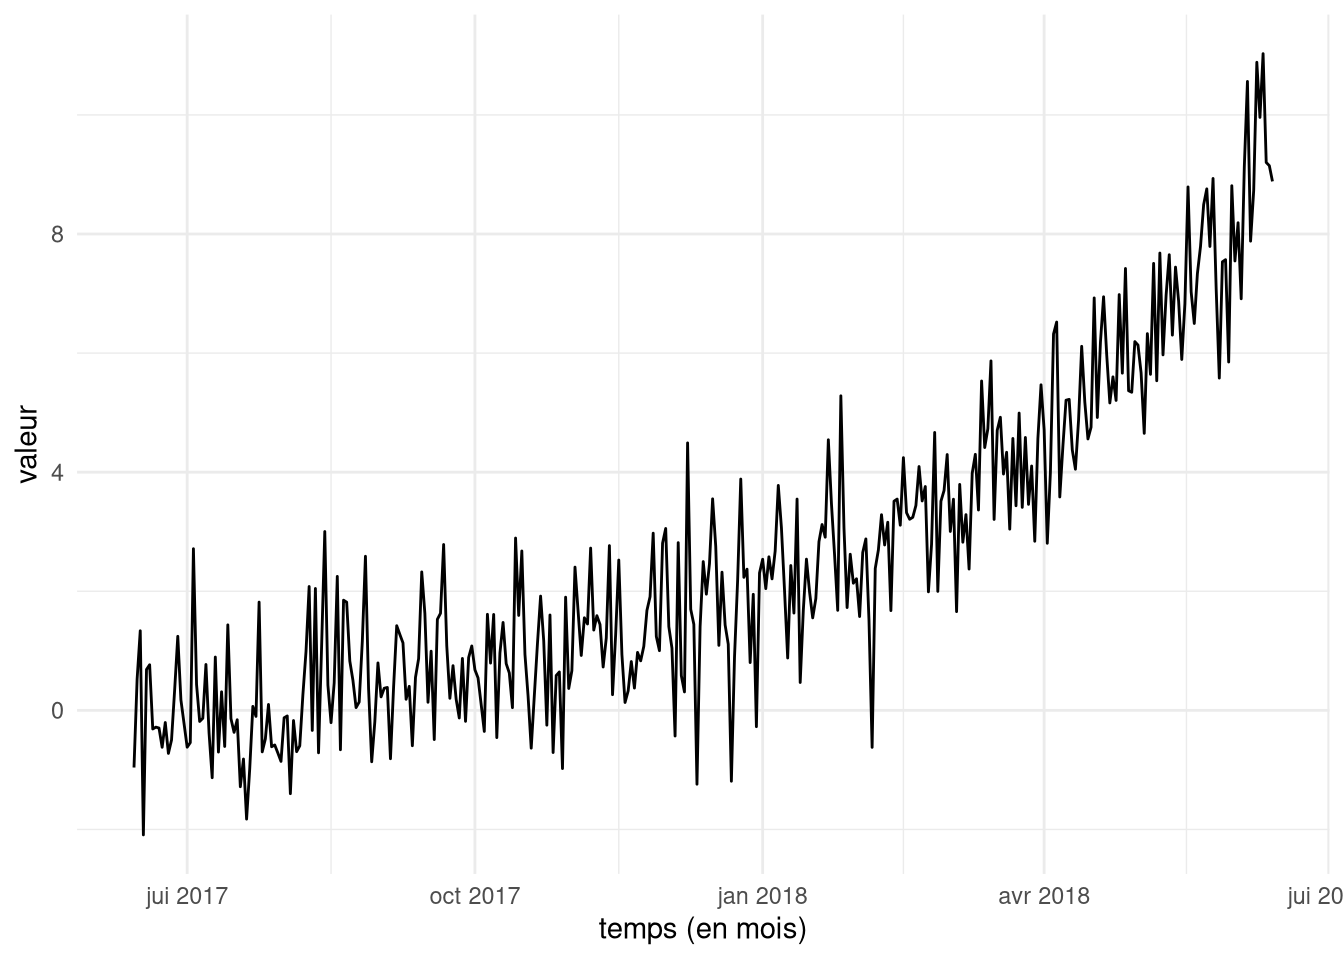
\includegraphics[width=0.7\linewidth]{MATH60604_Modelisation_statistique_files/figure-latex/seriechrono-1} 

}

\caption{Représentation graphique d'une série chronologique.}\label{fig:seriechrono}
\end{figure}

Plutôt que de décrire plus en détail le processus de l'analyse exploratoire, on présente un exemple qui illustre le cheminement habitue sur les données de trains de la Renfe introduites précédemment.

\begin{example}[Analyse exploratoire des trains Renfe]
\protect\hypertarget{exm:renfe-aed}{}{\label{exm:renfe-aed} \iffalse (Analyse exploratoire des trains Renfe) \fi{} }La première étape consisterait à lire la description de la base de données. Le jeu de données \texttt{renfe} contient les variables suivantes
\end{example}

\begin{itemize}
\tightlist
\item
  \texttt{prix}: prix du billet (en euros);
\item
  \texttt{dest}: indicateur binaire du trajet, soit de Barcelone vers Madrid (\texttt{0}) ou de Madrid vers Barcelone (\texttt{1});
\item
  \texttt{tarif}: variable catégorielle indiquant le tarif du billet, un parmi \texttt{AdultoIda}, \texttt{Promo} et \texttt{Flexible};
\item
  \texttt{classe}: classe du billet, soit \texttt{Preferente}, \texttt{Turista}, \texttt{TuristaPlus} ou \texttt{TuristaSolo};
\item
  \texttt{type}: variable catégorielle indiquant le type de train, soit Alta Velocidad Española (\texttt{AVE}), soit Alta Velocidad Española conjointement avec TGV (un partenariat entre la SNCF et Renfe pour les trains à destination ou en provenance de Toulouse) \texttt{AVE-TGV}, soit les trains régionaux \texttt{REXPRESS}; seuls les trains étiquetés \texttt{AVE} ou \texttt{AVE-TGV} sont des trains à grande vitesse.
\item
  \texttt{duree}: longueur annoncée du trajet (en minutes);
\item
  \texttt{jour} entier indiquant le jour de la semaine du départ allant de dimanche (\texttt{1}) à samedi (\texttt{7}).
\end{itemize}

Il n'y a pas de valeurs manquantes et un aperçu des données (\texttt{head(renfe)}) montre qu'elles sont en format long, ce qui veut dire que chaque ligne contient une seule valeur pour la variable réponse, ici le prix d'un billet de train. On entame l'analyse exploratoire avec des questions plutôt vagues, par exemple

\begin{enumerate}
\def\labelenumi{\arabic{enumi}.}
\tightlist
\item
  Quels sont les facteurs déterminant le prix et le temps de parcours?
\item
  Est-ce que le temps de parcours est le même peut importe le type de train?
\item
  Quelles sont les caractéristiques distinctives des types de train?
\item
  Quelles sont les principales différences entre les tarifs?
\end{enumerate}

À l'exception de \texttt{prix} et de \texttt{duree}, toutes les variables explicatives sont catégorielles et stockées sous forme de facteur (\texttt{factor}). S'il faut déclarer chacune de ces variables, on porte une attention particulière à \texttt{jour} pour éviter les mauvaises surprises ultérieures.

On peut utiliser \texttt{str} pour obtenir un aperçu des données; la fonction \texttt{summary} permet d'obtenir des statistiques descriptives selon que les variables sont continues (minimum, maximum, moyenne, quartiles) ou catégoriells (fréquence); la fonction rapport aussi le nombre de valeurs manquantes (\texttt{NA}) par variable.

La manipulation de variables dans des bases de données est parfois loin d'être toujours élégante en \textbf{R}: on accès aux variables avec \texttt{\$}, par exemple \texttt{renfe\$prix}. Une alternative plus lisible et modulaire est d'utiliser l'opérateur tuyau (\texttt{\%\textgreater{}\%}), qui permet de créer une chaîne logique de commandes; la fonction \texttt{count} sert à compter le nombre d'instance de chaque modalité (ces fonctionnalités ne sont pas disponibles dans \textbf{R} par défaut, mais avec les paquetages \texttt{tidyverse} ou l'alternative minimale \texttt{poorman}, préalablement chargée).

\begin{Shaded}
\begin{Highlighting}[]
\NormalTok{renfe }\SpecialCharTok{\%\textgreater{}\%} \FunctionTok{count}\NormalTok{(classe)}
\end{Highlighting}
\end{Shaded}

\begin{verbatim}
##        classe    n
## 1  Preferente  809
## 2     Turista 7197
## 3 TuristaPlus 1916
## 4 TuristaSolo   78
\end{verbatim}

\begin{Shaded}
\begin{Highlighting}[]
\CommentTok{\# un raccourci pour la même syntaxe}
\NormalTok{renfe }\SpecialCharTok{\%\textgreater{}\%} \FunctionTok{group\_by}\NormalTok{(type) }\SpecialCharTok{\%\textgreater{}\%} \FunctionTok{tally}\NormalTok{()}
\end{Highlighting}
\end{Shaded}

\begin{verbatim}
##       type    n
## 1      AVE 9174
## 2  AVE-TGV  429
## 3 REXPRESS  397
\end{verbatim}

\begin{Shaded}
\begin{Highlighting}[]
\NormalTok{renfe }\SpecialCharTok{\%\textgreater{}\%} \FunctionTok{group\_by}\NormalTok{(tarif) }\SpecialCharTok{\%\textgreater{}\%} \FunctionTok{tally}\NormalTok{()}
\end{Highlighting}
\end{Shaded}

\begin{verbatim}
##       tarif    n
## 1 AdultoIda  397
## 2  Flexible 1544
## 3     Promo 8059
\end{verbatim}

En analysant le nombre de trains dans les catégories, on remarque qu'il y a autant de billets de type \texttt{REXPRESS} que le nombre de billets au tarif \texttt{AdultoIda}. On peut faire le décompte par catégorie avec un tableau de contingence, qui compte le nombre respectif dans chaque sous-catégorie. Dans la base de données Renfe, tous les billets pour les RegioExpress sont vendus au tarif \texttt{AdultoIda} en classe \texttt{Turista}. Le nombre de billets est minime, à peine 397 sur 10000. Cela suggère une nouvelle question: pourquoi ces trains sont-ils si peu populaires?

\begin{verbatim}
##       tarif     type    n
## 1 AdultoIda REXPRESS  397
## 2  Flexible      AVE 1446
## 3  Flexible  AVE-TGV   98
## 4     Promo      AVE 7728
## 5     Promo  AVE-TGV  331
\end{verbatim}

On remarque également que seulement 17 temps de parcours sont affichés sur les billets (\texttt{renfe\ \%\textgreater{}\%\ distinct(duree)} ou \texttt{unique(renfe\$duree)}). On peut donc penser que la durée affichée sur le billet (en minutes) est le temps de trajet annoncé. La majeure partie (15 sur 17) des temps de parcours sont sous la barre des 3h15, hormis deux qui dépassent les 9h! Selon Google Maps, les deux villes sont distantes de 615km par la route, 500km à vol d'oiseau. Cela implique que, vraisemblablement, certains trains dépassent les 200km/h, tandis que d'autres vont plutôt à 70km/h. Quels sont ces trains plus lent? La variable \texttt{type} codifie probablement ce fait, et permet de voir que ce sont les trains RegioExpress qui sont dans cette catégorie.

\begin{Shaded}
\begin{Highlighting}[]
\NormalTok{renfe }\SpecialCharTok{\%\textgreater{}\%} 
  \FunctionTok{subset}\NormalTok{(duree }\SpecialCharTok{\textgreater{}} \DecValTok{200}\NormalTok{) }\SpecialCharTok{\%\textgreater{}\%} 
  \FunctionTok{group\_by}\NormalTok{(type, dest) }\SpecialCharTok{\%\textgreater{}\%} 
  \FunctionTok{summarise}\NormalTok{(}\StringTok{"durée moyenne"} \OtherTok{=} \FunctionTok{mean}\NormalTok{(duree), }
            \StringTok{"écart{-}type"} \OtherTok{=} \FunctionTok{sd}\NormalTok{(duree),}
            \StringTok{"prix moyen"} \OtherTok{=} \FunctionTok{mean}\NormalTok{(prix), }
            \StringTok{"écart{-}type"} \OtherTok{=} \FunctionTok{sd}\NormalTok{(prix)) }
\end{Highlighting}
\end{Shaded}

\begin{verbatim}
##       type             dest durée moyenne écart-type prix moyen écart-type
## 1 REXPRESS Barcelone-Madrid           544          0       43.2          0
## 2 REXPRESS Madrid-Barcelone           562          0       43.2          0
\end{verbatim}

Aller de Madrid à Barcelone à l'aide d'un train régulier prend 18 minutes de plus. Avec plus de 9h de trajet, pas étonnant donc que ces billets soient peu courus. Encore plus frappant, on note que le prix des billets est fixe: 43.25 euros peu importe que le trajet soit aller ou retour. C'est probablement la trouvaille la plus importante jusqu'à maintenant, car les billets de train de type RegioExpress ne forment pas un échantillon: il n'y a aucune variabilité! On aurait pu également découvrir cette anomalie en traçant une boîte à moustaches du prix en fonction du type de train.

\begin{figure}

{\centering 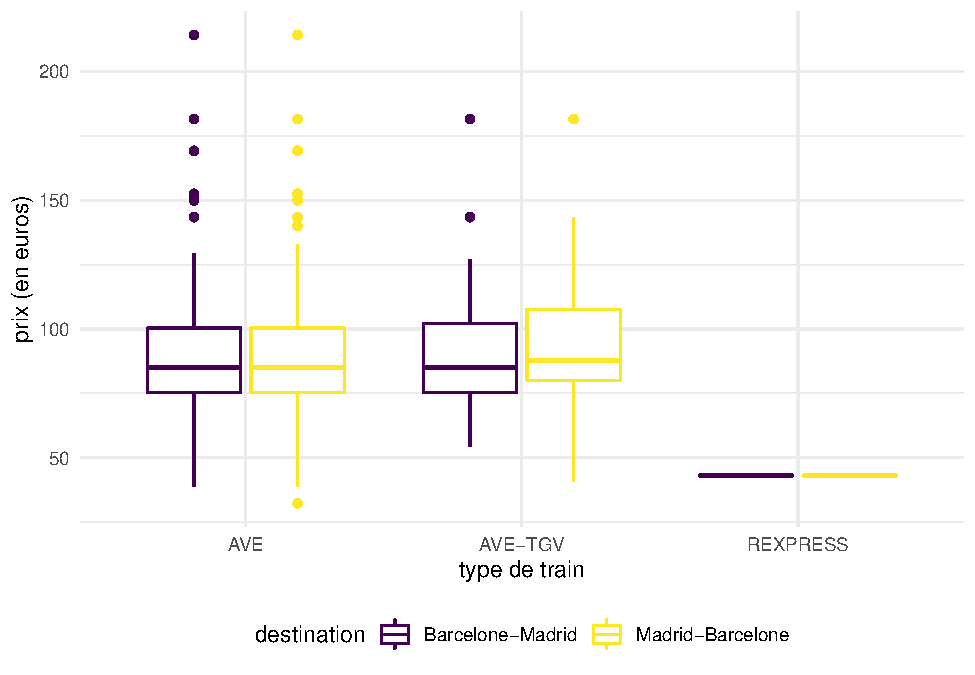
\includegraphics[width=0.7\linewidth]{MATH60604_Modelisation_statistique_files/figure-latex/renfe-aed4-1} 

}

\caption{Boîte à moustaches du prix de billets de train de Renfe en fonction de la destination et du type de train.}\label{fig:renfe-aed4}
\end{figure}

On pourrait soupçonner que les trains étiquetés \texttt{AVE} soient plus rapides, sachant que c'est l'acronyme de \emph{Alta Velocidad Española}, littéralement haute vitesse espagnole. Qu'en est-il des distinctions entre les deux types de trains étiquetés AVE? Selon \href{https://www.renfe-sncf.com/rw-en/services/a-unique-experience/Pages/services.aspx}{le site de la SNCF}, les trains AVE-TGV sont des partenariats entre la Renfe et la SNCF et effectuent des liaisons entre la France et l'Espagne.

\begin{Shaded}
\begin{Highlighting}[]
\NormalTok{renfe }\SpecialCharTok{\%\textgreater{}\%} 
  \FunctionTok{subset}\NormalTok{(type }\SpecialCharTok{\%in\%} \FunctionTok{c}\NormalTok{(}\StringTok{"AVE"}\NormalTok{,}\StringTok{"AVE{-}TGV"}\NormalTok{)) }\SpecialCharTok{\%\textgreater{}\%} 
  \FunctionTok{group\_by}\NormalTok{(type, dest) }\SpecialCharTok{\%\textgreater{}\%} 
  \FunctionTok{summarise}\NormalTok{(}\StringTok{"durée moyenne"} \OtherTok{=} \FunctionTok{mean}\NormalTok{(duree), }
            \StringTok{"écart{-}type"} \OtherTok{=} \FunctionTok{sd}\NormalTok{(duree),}
            \StringTok{"prix moyen"} \OtherTok{=} \FunctionTok{mean}\NormalTok{(prix),}
            \StringTok{"écart{-}type"} \OtherTok{=} \FunctionTok{sd}\NormalTok{(prix))}
\end{Highlighting}
\end{Shaded}

\begin{verbatim}
##      type             dest durée moyenne écart-type prix moyen écart-type
## 1     AVE Barcelone-Madrid           171       15.9       87.4       19.8
## 2     AVE Madrid-Barcelone           170       16.6       88.2       20.8
## 3 AVE-TGV Barcelone-Madrid           175        0.0       87.0       16.8
## 4 AVE-TGV Madrid-Barcelone           179        0.0       90.6       20.2
\end{verbatim}

Les prix sont beaucoup plus élevés, en moyenne plus de deux fois plus que les trains régionaux. Les écarts de prix importants (l'écart type est de 20 euros) indique qu'il y a peut-être d'autres sources d'hétérogénéité, mais on pourrait soupçonner que la Renfe pratique la tarification dynamique. Il y un seul temps de parcours prévu pour les trains AVE-TGV. On ne note pas de différence de prix notable selon la direction ou le type de train grande vitesse, mais peut-être que les tarifs ou la classe disponibles diffèrent selon que le train ou non est en partenariat avec la compagnie française.

On a pas encore considéré le tarif et la classe des billets, hormis pour les trains RegioExpress. On voit dans la Figure \ref{fig:renfe-aed7} une forte différente dans l'hétérogénéité des prix selon le tarif; le tarif Promo prend plusieurs valeurs distinctes, tandis que les tarifs AdultoIda et Flexible semblent ne prendre que quelques valeurs. La première classe (\texttt{Preferente}) est plus chère et il y a moins d'observations dans ce groupe. La classe Turista est la classe la moins dispendieuse et la plus populaire. \href{http://web.archive.org/web/20161111134241/http://www.renfe.com/viajeros/tarifas/billete_promo.html}{\texttt{TuristaPlus}} offre plus de confort, tandis que \texttt{TuristaSolo} permet d'obtenir un siège individuel.

Côté tarif, \href{http://web.archive.org/web/20161111134241/http://www.renfe.com/viajeros/tarifas/billete_promo.html}{Promo} et \href{http://web.archive.org/web/20161110220249/http://www.renfe.com/viajeros/tarifas/billete_promoplus.html}{PromoPlus} permette d'obtenir des rabais pouvant aller jusqu'à respectivement 70\% et 65\%. Les annulations et changements ne sont pas possibles avec Promo, mais disponibles avec PromoPlus moyennant une pénalité équivalent à 30-20\% du prix du billet. Le tarif \href{http://web.archive.org/web/20161108192609/http://www.renfe.com/viajeros/tarifas/billete_flexible.html}{Flexible} est disponible au même prix que les billets réguliers, avec des bénéfices additionnels.

\begin{Shaded}
\begin{Highlighting}[]
\NormalTok{renfe }\SpecialCharTok{\%\textgreater{}\%} \FunctionTok{subset}\NormalTok{(tarif  }\SpecialCharTok{!=} \StringTok{"AdultoIda"}\NormalTok{) }\SpecialCharTok{\%\textgreater{}\%}
\FunctionTok{ggplot}\NormalTok{(}\FunctionTok{aes}\NormalTok{(}\AttributeTok{y =}\NormalTok{ prix, }\AttributeTok{x =}\NormalTok{ classe, }\AttributeTok{col =}\NormalTok{ tarif)) }\SpecialCharTok{+} 
  \FunctionTok{geom\_boxplot}\NormalTok{() }\SpecialCharTok{+} 
  \FunctionTok{labs}\NormalTok{(}\AttributeTok{y =} \StringTok{"prix (en euros)"}\NormalTok{,}
       \AttributeTok{x =} \StringTok{"classe"}\NormalTok{,}
       \AttributeTok{color =} \StringTok{"tarif"}\NormalTok{) }\SpecialCharTok{+}
  \FunctionTok{theme}\NormalTok{(}\AttributeTok{legend.position =} \StringTok{"bottom"}\NormalTok{)}
\end{Highlighting}
\end{Shaded}

\begin{figure}

{\centering 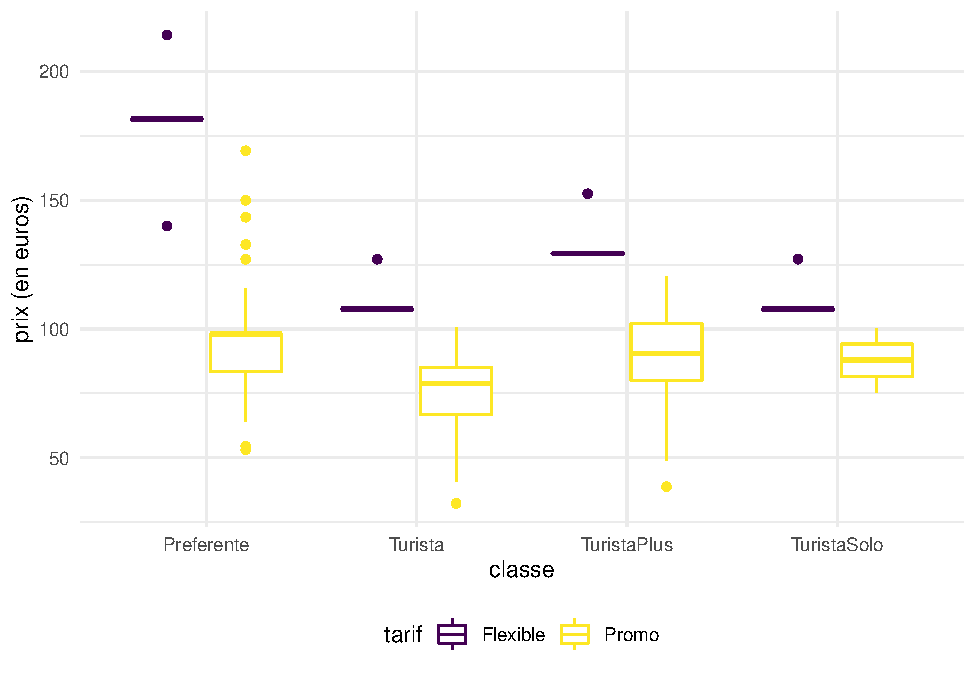
\includegraphics[width=0.7\linewidth]{MATH60604_Modelisation_statistique_files/figure-latex/renfe-aed6-1} 

}

\caption{Boîte à moustaches du prix en fonction du tarif et de la classe de billets de trains à haute vitesse de la Renfe.}\label{fig:renfe-aed6}
\end{figure}

\begin{Shaded}
\begin{Highlighting}[]
\FunctionTok{ggplot}\NormalTok{(}\AttributeTok{data =}\NormalTok{ renfe, }\FunctionTok{aes}\NormalTok{(}\AttributeTok{x =}\NormalTok{ prix, }\AttributeTok{y=}\NormalTok{..density.., }\AttributeTok{fill =}\NormalTok{ tarif)) }\SpecialCharTok{+}
    \FunctionTok{geom\_histogram}\NormalTok{(}\AttributeTok{binwidth =} \DecValTok{5}\NormalTok{) }\SpecialCharTok{+}
    \FunctionTok{labs}\NormalTok{(}\AttributeTok{x =} \StringTok{"prix (en euros)"}\NormalTok{, }\AttributeTok{y =} \StringTok{"densité"}\NormalTok{) }\SpecialCharTok{+} 
    \FunctionTok{theme}\NormalTok{(}\AttributeTok{legend.position =} \StringTok{"bottom"}\NormalTok{)}
\end{Highlighting}
\end{Shaded}

\begin{figure}

{\centering 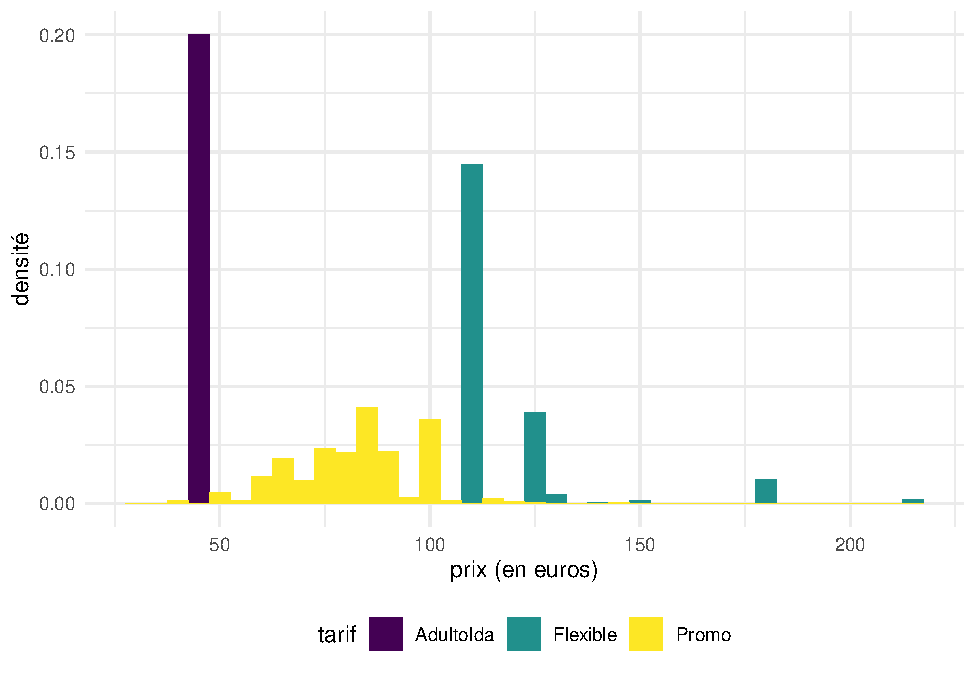
\includegraphics[width=0.7\linewidth]{MATH60604_Modelisation_statistique_files/figure-latex/renfe-aed7-1} 

}

\caption{Histogrammes du prix en fonction du tarif de billets de trains de la Renfe.}\label{fig:renfe-aed7}
\end{figure}

\begin{Shaded}
\begin{Highlighting}[]
\CommentTok{\# Vérifier la répartition des billets Flexible}
\NormalTok{renfe }\SpecialCharTok{\%\textgreater{}\%} \FunctionTok{subset}\NormalTok{(tarif  }\SpecialCharTok{==} \StringTok{"Flexible"}\NormalTok{) }\SpecialCharTok{\%\textgreater{}\%} \FunctionTok{count}\NormalTok{(prix, classe)}
\end{Highlighting}
\end{Shaded}

\begin{verbatim}
##   prix      classe    n
## 1  108     Turista 1050
## 2  108 TuristaSolo   67
## 3  127     Turista  285
## 4  127 TuristaSolo    9
## 5  129 TuristaPlus   31
## 6  140  Preferente    2
## 7  152 TuristaPlus   10
## 8  182  Preferente   78
## 9  214  Preferente   12
\end{verbatim}

On note que la répartition des prix pour les billets de classe Flexible est inhabituelle: notre boîte à moustachesest écrasée et l'écart interquartile semble nul, même si quelques valeurs inexpliquées sont aussi présentes. L'écrasante majorité des billets Flexibles sont en classe Turista, donc ça pourrait être dû à un (trop) faible nombre de billets dans chaque catégorie. On peut rejeter cette hypothèse en calculant le nombre de trains au tarif Flexible pour les différents types de billets. Ni la durée, ni le type de train, ni la destination n'expliquent pas pourquoi le prix de certains billets Flexibles est plus faible ou élevés. Le prix des billets Promo est plus faible, et les billets au tarif Preferente (la première classe) sont plus élevés.

On peut résumer notre brève analyse exploratoire:

\begin{itemize}
\tightlist
\item
  plus de 91\% des trains sont des trains à grande vitesse AVE.
\item
  le temps de trajet dépend du type de train: les trains à grande vitesse mettent 3h20 au maximum pour relier Madrid et Barcelone.
\item
  les temps de trajets sont ceux annoncés (variable discrète avec 17 valeurs uniques, dont 13 pour les trains AVE)
\item
  le prix de trains RegioExpress est fixe (43.25€); tous ces billets sont dans la classe Turista et au tarif Adulto Ida. 57\% de ces trains vont de Barcelone à Madrid. La durée du trajet pour les RegioExpress est de 9h22 de Barcelona à Madrid, 18 minutes de plus que dans l'autre direction.
\item
  les billets en classe\texttt{Preferente} sont plus chers et moins fréquents. La classe \texttt{Turista} est la classe la moins dispendieuse et la plus populaire. \texttt{TuristaPlus} offre plus de confort, tandis que \texttt{TuristaSolo} permet d'obtenir un siège individuel.
\item
  selon le \href{https://www.renfe.com/es/es/viajar/tarifas/billetes.html}{site web de la Renfe}, les billets au tarif \texttt{Flexible} « viennent avec des offres additionnelles qui permettent au passagers d'échanger leurs billets ou annuler s'ils manquent leurs trains. »; en contrepartie, ces billets sont plus chers et leur tarif est fixe sauf une poignée de billets dont le prix reste inexpliqué.
\item
  la distribution des prix des billets de TGV au tarif \texttt{Promo} est plus ou moins symmétrique, tandis que les billets au tarif \texttt{Flexible} apparaissent tronqués à gauche (le prix minimum pour ces billets est 107.7€ dans l'échantillon).
\item
  la Renfe pratique la tarification dynamique pour les billets au tarif promotionnel \texttt{Promo}: ces derniers peuvent être jusqu'à 70\% moins chers que les billets à prix régulier lorsqu'achetés via l'agence officielle ou le site de Renfe. Ces billets ne peuvent être ni remboursés, ni échangés.
\item
  il n'y a pas d'indication à effet de quoi les prix varient selon la direction du trajet.
\end{itemize}

\hypertarget{regression-lineaire}{%
\section{Régression linéaire}\label{regression-lineaire}}

On entend par régression linéaire un modèle pour l'espérance conditionnelle d'une variable réponse \(Y\) (ou régressande) en fonction de \(p\) variables explicatives (appelées parfois régresseurs ou covariables) à l'aide d'une équation de la forme
\begin{align*}
\mathsf{E}(Y \mid \mathbf{X})=\beta_0 + \beta_1\mathrm{X}_{1} + \cdots + \beta_p \mathrm{X}_{p}.
\end{align*}
Le fait que la moyenne est conditionnelle aux valeurs de \(\mathbf{X}\) implique simplement que l'on considère les régresseurs comme constant, ou connus à l'avance.

En pratique, tout modèle est une approximation de la réalité, aussi on ajoute un terme d'erreur qui sert à tenir compte du fait qu'aucune relation linéaire exacte ne lie \(\mathbf{X}\) et \(Y\), ou que les mesures de \(Y\) contiennent des erreurs. Ce terme d'erreur aléatoire \(\varepsilon\) servira de base à l'inférence car il permettra de quantifier l'adéquation entre notre modèle et les données.

On peut réécrire le modèle linéaire en terme de l'erreur pour un échantillon aléatoire de taille \(n\): dénotons par \(Y_i\) la valeur de \(Y\) pour le sujet \(i\), et \(\mathrm{X}_{ij}\) la valeur de la \(j\)e variable explicative du sujet \(i\). Le modèle de régression linéaire est
\begin{align}
Y_i = \beta_0 + \beta_1 \mathrm{X}_{i1} + \ldots + \beta_p \mathrm{X}_{ip} +\varepsilon_{i}, \qquad i =1, \ldots, n, \label{eq:olsmean}
\end{align}
où \(\varepsilon_i\) est le terme d'erreur additive. Si aucune hypothèse sur la loi aléatoire de l'erreur n'est spécifiée, on fixe néanmoins l'espérance du terme d'erreur à zéro car on postule qu'il n'y a pas d'erreur systématique, c'est-à-dire que \(\mathsf{E}(\varepsilon_i \mid \boldsymbol{X}_i)=0\) \((i=1, \ldots, n)\).

La flexibilité du modèle linéaire vient de sa formulation: on spécifie l'espérance conditionnelle d'une variable continue comme \textbf{combinaison linéaire de variables explicatives}, dont le choix est arbitraire.
Il est important de remarquer que ce modèle est linéaire dans les coefficients \(\boldsymbol{\beta}\in \mathbb{R}_{p+1}\), pas dans les variables explicatives! les covariables sont quelconques et peuvent être des fonctions (non)-linéaires d'autres variables explicatives, par exemple \(\mathrm{X}=\log(\texttt{annees})\), \(\mathrm{X}=\texttt{puissance}^2\) ou \(\mathrm{X}= \mathsf{I}_{\texttt{homme}}\cdot\mathsf{I}_{\texttt{titulaire}}\). C'est ce qui fait la flexibilité du modèle linéaire: ce dernier est principalement employé aux fins suivantes:

\begin{enumerate}
\def\labelenumi{\arabic{enumi}.}
\tightlist
\item
  Comprendre comment et dans quelle mesure les variables explicatives \(\mathbf{X}\) influencent la moyenne de la réponse \(Y\) (description).
\item
  Quantifier l'influence des variables explicatives \(\mathbf{X}\) sur la régressande \(Y\) et tester leur significativité.
\item
  Prédire les valeurs de \(Y\) pour de nouveaux ensembles de covariables \(\mathbf{X}\).
\end{enumerate}

\hypertarget{introduction}{%
\subsection{Introduction}\label{introduction}}

Le modèle linéaire est sans conteste le modèle statistique le plus couramment employé. Le terme « modèle linéaire » est trompeur: une grande panoplie de tests statistiques (tests-\emph{t}, analyse de variance, test de Wilcoxon ou de Kruskal--Wallis) \href{https://lindeloev.github.io/tests-as-linear/linear_tests_cheat_sheet.pdf}{peut être calculée à l'aide d'un modèle linéaire}, tandis que \href{https://threadreaderapp.com/thread/1286420597505892352.html}{des modèles aussi divers que les arbres aléatoires, la régression en composantes principales et les réseaux de neurones multicouches ne sont en réalité que de bêtes modèles linéaires}. Ce qui change d'un modèle à l'autre est simplement la méthode d'optimisation (moindres carrés ordinaires, optimisation sous contrainte ou par descente de gradient stochastique), de même que le choix des variables explicatives (bases de spline pour la régression nonparamétrique, variables indicatrices pour les arbres, fonctions d'activations pour les réseaux de neurones). Ce chapitre porte sur la formulation de modèles linéaires, l'interprétation des coefficients et les tests usuels reliés à ces modèles. Certains modèles bien connus, comme l'analyse de variance, seront présentés comme cas spéciaux du modèle de régression linéaire.

Afin de rendre plus tangible le concept et les notions qui touchent aux modèles linéaires, on présentera ces notions dans le cadre d'un exemple. On s'intéresse à la discrimination salariale dans un collège américain, au sein duquel une étude a été réalisée pour investiguer s'il existait des inégalités salariales entre hommes et femmes. Le jeu de données contient les variables suivantes

\begin{itemize}
\tightlist
\item
  \texttt{salaire}: salaire de professeurs pendant l'année académique 2008--2009 (en milliers de dollars USD).
\item
  \texttt{echelon}: échelon académique, soit adjoint (\texttt{adjoint}), aggrégé (\texttt{aggrege}) ou titulaire (\texttt{titulaire}).
\item
  \texttt{domaine}: variable catégorielle indiquant le champ d'expertise du professeur, soit appliqué (\texttt{applique}) ou théorique (\texttt{theorique}).
\item
  \texttt{sexe}: indicateur binaire pour le sexe, \texttt{homme} ou \texttt{femme}.
\item
  \texttt{service}: nombre d'années de service.
\item
  \texttt{annees}: nombre d'années depuis l'obtention du doctorat.
\end{itemize}

Une analyse exploratoire des données est de mise avant d'ébaucher un modèle. Si le salaire augmente au fil des ans, on voit que l'hétérogénéité change en fonction de l'échelon et qu'il y a une relation claire entre ce dernier et le nombre d'années de service (les professeurs n'étant éligibles à des promotions qu'après un certain nombre d'années). Les professeurs adjoints qui ne sont pas promus sont généralement mis à la porte, aussi il y a moins d'occasions pour que les salaires varient sur cette échelle.

\begin{figure}

{\centering 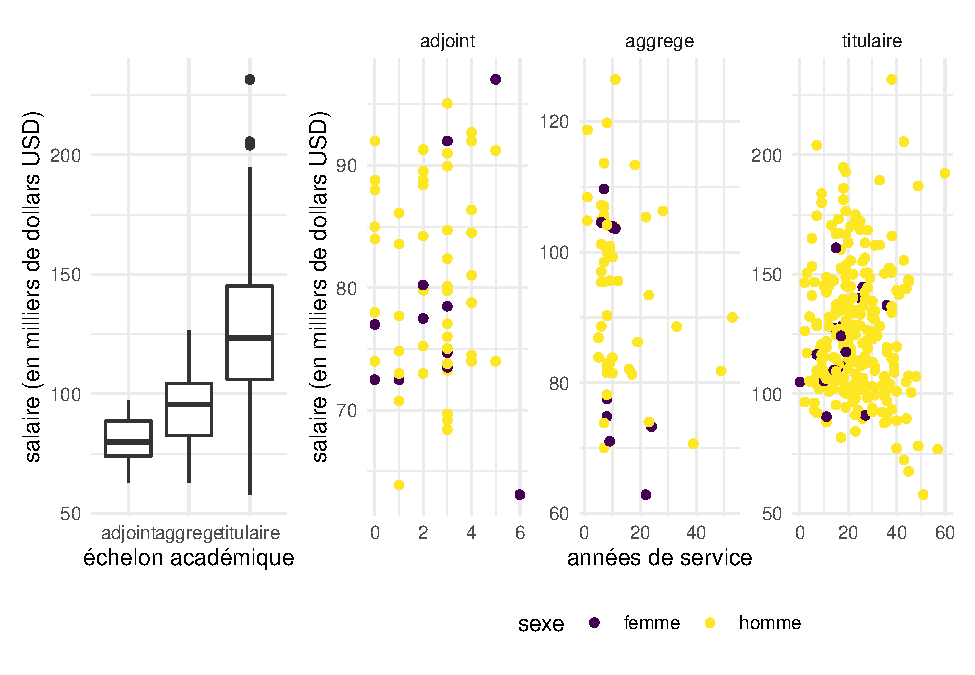
\includegraphics[width=0.7\linewidth]{MATH60604_Modelisation_statistique_files/figure-latex/edacollege-1} 

}

\caption{Analyse exploratoire des données $\texttt{college}$: répartition des salaires en fonction de l'échelon et du nombre d'années de service}\label{fig:edacollege}
\end{figure}

Ainsi, le salaire augmente avec les années, mais la variabilité croît également. Il y a peu de femmes dans l'échantillon: moins d'information signifie moins de puissance pour détecter de petites différences de salaire. Si on fait un tableau de contingence de l'échelon et du sexe, on peut calculer la proportion relative homme/femme dans chaque échelon: 16\% des profs adjoints, 16\% pour les aggrégés, mais seulement 7\% des titulaires alors que ces derniers sont mieux payés en moyenne.

\begin{table}

\caption{\label{tab:tableaucontingence}Tableau de contingence donnant le nombre de professeurs du collège par sexe et par échelon académique.}
\centering
\begin{tabular}[t]{lrrr}
\toprule
  & adjoint & aggrege & titulaire\\
\midrule
femme & 11 & 10 & 18\\
homme & 56 & 54 & 248\\
\bottomrule
\end{tabular}
\end{table}

Le modèle linéaire simple n'inclut qu'une variable explicative et consiste en une droite d'équation \(y=\beta_0 + \beta_1 \mathrm{X}\) qui passe à travers un nuage de points. La Figure \ref{fig:droitenuage} montre la droite de régression dans le nuage de points formé par les couples \(\{\mathrm{X}_i, y_i\}\), où \(y_i\) est le \texttt{salaire} et \(\mathrm{X}\) est \texttt{service}.

\begin{figure}

{\centering 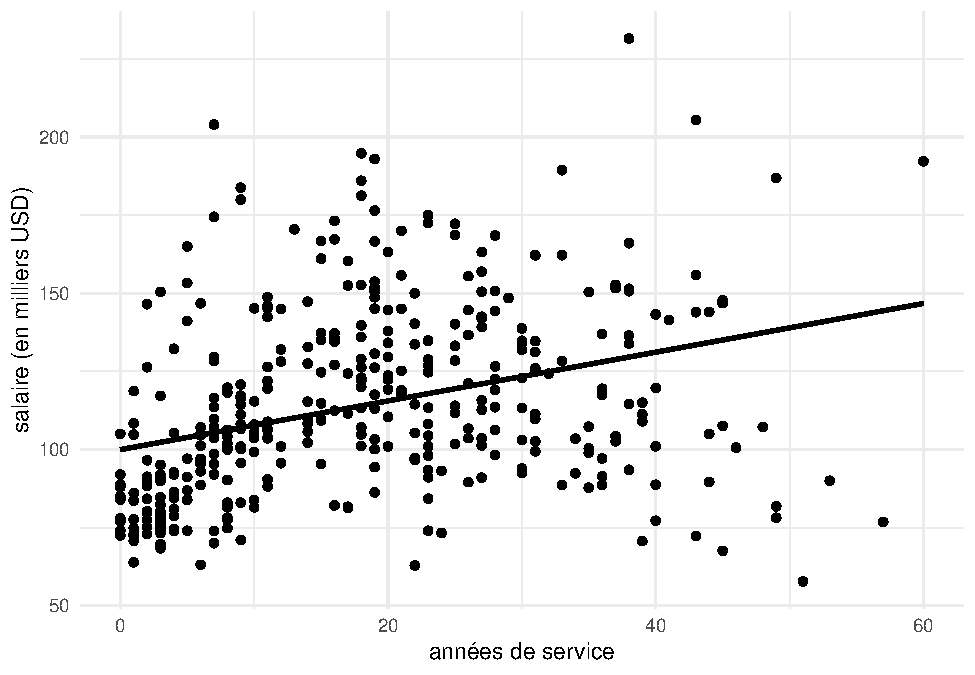
\includegraphics[width=0.7\linewidth]{MATH60604_Modelisation_statistique_files/figure-latex/droitenuage-1} 

}

\caption{Régression linéaire simple pour le salaire en fonction des années de service; la droite satisfait le critère des moindres carrés.}\label{fig:droitenuage}
\end{figure}

Une infinité de droites pourraient passer dans le nuage de points; il faut donc choisir la meilleure droite (selon un critère donné). La section aborde le choix de ce critère et l'estimation des paramètres de l'équation de la droite.

\hypertarget{moindres-carruxe9s-ordinaires}{%
\subsection{Moindres carrés ordinaires}\label{moindres-carruxe9s-ordinaires}}

Les estimateurs des moindres carrés ordinaires \(\widehat{\boldsymbol{\beta}}=(\widehat{\beta}_0, \ldots, \widehat{\beta}_p)\) sont les paramètres qui minimisent simultanément la distance euclidienne entre les observations \(Y_i\) et les \textbf{valeurs ajustées}
\begin{align*}
 \widehat{Y}_i &= \widehat{\beta}_0 + \widehat{\beta}_1 \mathrm{X}_{i1} + \cdots + \widehat{\beta}_p \mathrm{X}_{ip}, \qquad i =1, \ldots, n.
\end{align*}
En d'autres mots, les estimateurs des moindres carrés sont la solution du problème d'optimization convexe
\begin{align*}
\widehat{\boldsymbol{\beta}} &=\min_{\boldsymbol{\beta} \in \mathbb{R}^{p+1}}\sum_{i=1}^n (Y_i-\widehat{Y}_i)^2= \min_{\boldsymbol{\beta}} \|\boldsymbol{Y}-\mathbf{X}\boldsymbol{\beta}\|^2
\end{align*}
Ce système d'équation a une solution explicite qui est plus facilement exprimée en notation matricielle. Soit les matrices et vecteurs
\begin{align*}
\boldsymbol{Y} =
 \begin{pmatrix}
  Y_1 \\
  Y_2 \\
  \vdots \\
  Y_n 
 \end{pmatrix} ,
 \;
 \boldsymbol{\varepsilon} =
 \begin{pmatrix}
  \varepsilon_1 \\
  \varepsilon_2 \\
  \vdots \\
  \varepsilon_n 
 \end{pmatrix} ,
 \;
\mathbf{X} = \begin{pmatrix}
\mathrm{X}_{11} & \mathrm{X}_{12} & \cdots & \mathrm{X}_{1p} \\
\mathrm{X}_{21} & \mathrm{X}_{22} & \cdots & \mathrm{X}_{2p} \\
\vdots & \vdots & \ddots & \vdots \\
\mathrm{X}_{n1} & \mathrm{X}_{n2} & \cdots & \mathrm{X}_{np} 
\end{pmatrix} , \;
\boldsymbol{\beta} =
 \begin{pmatrix}
  \beta_1 \\
  \beta_2 \\
  \vdots \\
  \beta_p 
 \end{pmatrix}
\end{align*}
Le modèle en notation matricielle s'écrit de manière compacte, \begin{align*}
\boldsymbol{Y} = \mathbf{X} \boldsymbol{\beta} + \boldsymbol{\varepsilon};
\end{align*}
chaque ligne de la matrice correspond à l'équation \eqref{eq:olsmean} avec une observation par ligne.
L'estimateur des moindres carrés ordinaires résoud le problème d'optimisation non-contraint
\begin{align*}
\widehat{\boldsymbol{\beta}}=\min_{\boldsymbol{\beta} \in \mathbb{R}^{p+1}}(\boldsymbol{y}-\mathbf{X}\boldsymbol{\beta})^\top(\boldsymbol{y}-\mathbf{X}\boldsymbol{\beta}).
\end{align*}
Une preuve est fournie \protect\hyperlink{ols}{dans l'Annexe}. Si le rang de la matrice \(\mathbf{X}\) est dimension \(n \times (p+1)\) est de rang \(p+1\), l'unique solution du problème d'optimisation est
\begin{align}
\widehat{\boldsymbol{\beta}} = (\mathbf{X}^{\top} \mathbf{X})^{-1} \mathbf{X}^{\top} \boldsymbol{Y}. \label{eq:ols}
\end{align}

Que représente les moindres carrés en deux dimensions? L'estimateur est celui qui minimise la somme du carré des résidus ordinaires. Le \(i\)e \textbf{résidu ordinaire} \(e_i = y_i -\widehat{y}_i\) est la distance \emph{verticale} entre un point \(y_i\) et la valeur ajustée \(\widehat{y}_i\), soit les traits bleus de la Figure \ref{fig:distancevert}.

\begin{figure}

{\centering 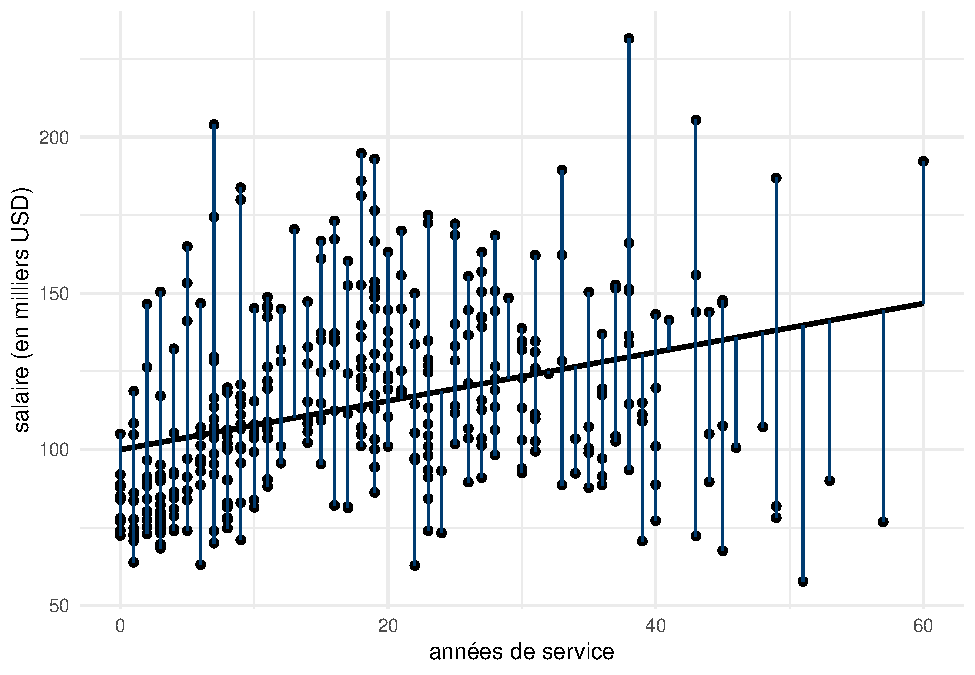
\includegraphics[width=0.7\linewidth]{MATH60604_Modelisation_statistique_files/figure-latex/distancevert-1} 

}

\caption{Illustration des résidus ordinaires ajoutés à la droite de régression.}\label{fig:distancevert}
\end{figure}

\begin{remark}[Géométrie des moindres carrés]
\iffalse{} {Remarque (Géométrie des moindres carrés). } \fi{}Si on considère les \(n\) observations comme un vecteur (colonne), le terme \(\mathbf{X} \widehat{\boldsymbol{\beta}}\) correspond à la projection sur l'espace linéaire engendré par les colonnes de la matrice \(\mathbf{X}\), \(\mathscr{S}_{\mathbf{X}}\) du vecteur de réponse \(\boldsymbol{y}\). Les résidus ordinaires sont donc orthogonaux à \(\mathscr{S}_{\mathbf{X}}\) par construction et les résidus sont orthogonaux aux valeurs ajustées, \(\boldsymbol{e}^\top\widehat{\boldsymbol{y}}=0\).
Une conséquence directe est que la corrélation linéaire entre \(\boldsymbol{e}\) et \(\widehat{\boldsymbol{y}}\) est zéro; cette propriété nous servira dans les diagnostics graphiques.
\end{remark}

\begin{remark}[Complexité du calcul des moindres carrés ordinaires]
\iffalse{} {Remarque (Complexité du calcul des moindres carrés ordinaires). } \fi{}Tangente: en apprentissage automatique, on utilise souvent un algorithme du gradient (stochastique) pour estimer les estimés des moindres carrés ordinaires. Or, à moins d'avoir des tailles d'échantillons \(n\) ou un nombre de covariables \(p\) subséquent (pensez échelle Google), une solution approximative ne devrait pas être préférée à la solution exacte! D'un point de vue numérique, l'opération la plus coûteuse est le calcul de l'inverse de la matrice \(\mathbf{X}^\top\mathbf{X}\), qui de dimension \((p+1) \times (p+1)\). Règle générale, on n'inverse pas directement cette matrice car ce n'est pas la façon la plus numériquement stable d'obtenir la solution. \textbf{R} utilise la décomposition QR qui a une complexité de \(\mathrm{O}(np^2)\) (l'ordre du nombre de flops ou d'opérations pour le calcul). Une alternative plus coûteuse, mais plus stable numériquement, est la décomposition en valeurs singulières (même ordre en terme de calculs).
\end{remark}

Mais trève de disgression mathématique: tout bon logiciel calculera pour vous les estimés des moindres carrés. Retenez que l'on minimise une forme quadratique qui admet une solution explicite et unique pour autant que les colonnes de \(\mathbf{X}\) ne soient pas colinéaires. Si vous avez plus d'une variable explicative, les valeurs ajustées seront situées sur un hyperplan (peu commode à représenter graphiquement). Maîtriser le langage associé à la régression (notamment les résidus ordinaires, les valeurs ajustées, etc.) est nécessaire pour la continuation.

\hypertarget{interpruxe9tation-des-paramuxe8tres-du-moduxe8les}{%
\subsection{Interprétation des paramètres du modèles}\label{interpruxe9tation-des-paramuxe8tres-du-moduxe8les}}

Que représentent les paramètres \(\boldsymbol{\beta}\) du modèle linéaire? Dans le cas simple présenté dans la Figure \ref{fig:droitenuage} où l'équation de la droite est de la forme \(\widehat{Y} = \widehat{\beta}_0 + \widehat{\beta}_1\mathrm{X}_1\), \(\beta_0\) est l'ordonnée à l'origine (la valeur moyenne de \(Y\) quand \(\mathrm{X}_1=0\)) et \(\beta_1\) est la pente, soit l'augmentation moyenne de \(Y\) quand \(\mathrm{X}_1\) augmente d'une unité.

Dans certains cas, l'interprétation de l'ordonnée à l'origine n'est pas valide car c'est un \textbf{non-sens}: la valeur \(\mathrm{X}_1=0\) n'est pas plausible (par exemple, si \(\mathrm{X}_1\) est la taille d'un humain). De même, il peut arriver qu'il n'y ait pas d'observations dans le voisinage de \(\mathrm{X}_1=0\), même si cette valeur est plausible; on parle alors d'extrapolation.

Si les colonnes de \(\mathbf{X}\) sont arbitraires, il est d'usage d'inclure une constante: cela revient à inclure \(\mathbf{1}_n\) comme colonne de la matrice de plan d'expérience \(\mathbf{X}\). Parce que les résidus sont orthogonaux aux colonnes de \(\mathbf{X}\), leur moyenne est zéro, \(n^{-1}\mathbf{1}_n^\top\boldsymbol{e}=\bar{\boldsymbol{e}}=0\). En général, on peut obtenir des résidus centrés en incluant comme régresseurs dans la matrice \(\mathbf{X}\) des vecteurs colonnes qui sont collinéaires avec \(\mathbf{1}_n\).

Dans notre exemple, l'équation de la droite ajustée de la Figure \ref{fig:droitenuage} est \[\widehat{\texttt{salaire}} = 99.975 + 0.78\texttt{service}.\]
Ainsi, le salaire moyen d'un nouveau professeur serait 99974.653 dollars, tandis que l'augmentation moyenne annuelle du salaire est 779.569 dollars.

Si la variable réponse \(Y\) doit être \emph{continue}, il n'y a aucune restriction pour les variables explicatives. Le cas des variables explicatives binaires est illustratif: ces variables sont encodées numériquement à l'aide de 0/1. Considérons par exemple le sexe des professeurs de l'étude, par exemple
\[\texttt{sexe} = \begin{cases} 0 , & \text{pour les hommes},\\
1, & \text{pour les femmes.}
\end{cases}
\]
L'équation du modèle linéaire simple qui n'inclut que cette variable catégorielle à deux niveaux, \(\texttt{sexe}\), s'écrit \(\texttt{salaire} = \beta_0 + \beta_1 \texttt{sexe} + \varepsilon\). Posons \(\mu_0\) le salaire moyen des hommes et \(\mu_1\) celui des femmes. L'ordonnée à l'origine \(\beta_0\) s'interprète comme d'ordinaire: c'est le salaire moyen quand \(\texttt{sexe}=0\), autrement dit \(\beta_0=\mu_0\). On peut écrire l'équation de l'espérance conditionnelle pour chacune des catégories,
\begin{align*}
\mathsf{E}(\texttt{salaire} \mid \texttt{sexe})= \begin{cases}
\beta_0, & \texttt{sexe}=0 \text{ (homme)}, \\
\beta_0 + \beta_1 & \texttt{sexe}=1 \text{ (femme)}.
\end{cases}
\end{align*}
Un modèle linéaire qui contient uniquement une variable binaire \(\mathrm{X}\) comme régresseur équivaut à spécifier une moyenne différente pour deux groupes; la moyenne des femmes est \(\mathsf{E}(\texttt{salaire} \mid \texttt{sexe}=1) = \beta_0 + \beta_1 = \mu_1\) et \(\beta_1=\mu_1-\mu_0\) représente la différence entre la moyenne des hommes et celles des femmes. L'estimateur des moindres carrés \(\widehat{\beta}_0\) est la moyenne du salaire des hommes de l'échantillon et \(\widehat{\beta}_1\) est la différence des moyennes empiriques entre femmes et hommes. Cette paramétrisation en terme d'\textbf{effets différentiels} est particulièrement utile si on veut tester s'il y a une différence moyenne de salaire entre les deux sexe car cela revient à tester \(\mathscr{H}_0: \beta_1=0\). Si on voulait obtenir directement la moyenne, il faudrait remplacer la matrice de plan d'expérience \([\mathbf{1}_n, \texttt{sexe}]\) par \([\mathbf{1}_n- \texttt{sexe}, \texttt{sexe}]\) pour obtenir un modèle équivalent. Règle générale, il n'est pas recommandé de retirer l'ordonnée à l'origine même si l'espace linéaire engendré par les colonnes de \(\mathbf{X}\) contient \(\mathbf{1}_n\).

\begin{figure}

{\centering 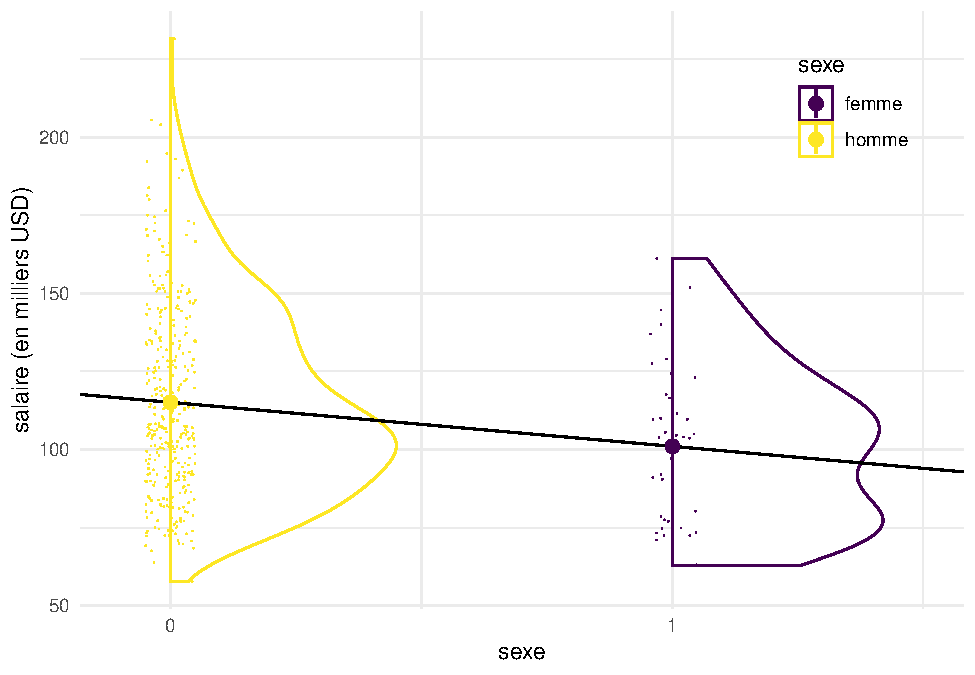
\includegraphics[width=0.7\linewidth]{MATH60604_Modelisation_statistique_files/figure-latex/graphcollegesexe-1} 

}

\caption{Modèle linéaire simple pour les données $\texttt{college}$ en fonction de la variable binaire sexe: bien que le modèle définisse une ligne, seule la valeur en $0/1$ est réalisable.}\label{fig:graphcollegesexe}
\end{figure}

Si on ajuste un modèle de régression linéaire pour les données \texttt{college}, on obtient un salaire moyen de \(\widehat{\beta}_0=115.09\) milliers de dollars USD pour les hommes et une différence moyenne de salaire entre femmes et hommes de \(\widehat{\beta}_1=14.088\) milliers de dollars. Puisque l'estimé est négatif, les femmes sont moins payés: ce modèle n'est en revanche pas suffisant pour déterminer s'il y a inéquité salariale: la Figure \ref{fig:droitenuage} montre que le nombre d'années de service et l'échelon académique impactent fortement le salaire, or il n'est pas dit que la répartition des sexes au sein des échelons est comparable (et ce n'est pas le cas).

Même si le modèle linéaire simple définit une droite, cette dernière n'a de sens qu'en \(0\) ou \(1\); la Figure \ref{fig:graphcollegesexe} montre un estimé de la densité et la répartition des points (décalés) dans l'échantillon selon le sexe, avec la moyenne de chacun. On voit bien que la droite passe par la moyenne de chaque groupe.

Plus généralement, il est possible de considérer une variable catégorielle à \(k\) niveaux. Comme pour la variable binaire, on ajoute au modèle \(k-1\) variables indicatrices en plus de l'ordonnée à l'origine: si on veut modéliser \(k\) moyennes, il est logique de n'inclure que \(k\) paramètres. On choisira comme dans l'exemple avec le sexe une \textbf{catégorie de référence} dont la moyenne sera encodée par l'ordonnée à l'origine \(\beta_0\). Les autres paramètres seront des effets différentiels relatifs à cette catégorie. Prenons pour exemple l'échelon académique, une variable catégorielle ordinale à trois niveaux (adjoint, aggrégé, titulaire). On ajoute deux variables binaires \(\mathrm{X}_1 = \mathsf{I}(\texttt{echelon}=\texttt{aggrege})\) et \(\mathrm{X}_2 = \mathsf{I}(\texttt{echelon}=\texttt{titulaire})\); l'élément \(i\) de la colonne \(\mathrm{X}_1\) vaut 1 si le professeur est aggrégé et zéro autrement. Le modèle linéaire
\begin{align*}
\texttt{salaire} \mid \texttt{echelon}=\beta_0 + \beta_1 \mathrm{X}_1+\beta_2\mathrm{X}_2 + \varepsilon,
\end{align*}
et l'espérance conditionnelle du salaire s'écrit
\begin{align*}
\mathsf{E}(\texttt{salaire} \mid \texttt{echelon})= \begin{cases}
\beta_0, & \texttt{echelon}=\texttt{adjoint},\\
\beta_0 + \beta_1 & \texttt{echelon}=\texttt{aggrege},\\
\beta_0 + \beta_2 & \texttt{echelon}=\texttt{titulaire},
\end{cases}
\end{align*}
Ainsi, \(\beta_1\) (respectivement \(\beta_2\)) est la différence de salaire moyenne entre professeurs titulaires (respectivement aggrégés) et professeurs adjoints.
Le choix de la catégorie de référence est arbitraire et le modèle ajusté est le même: seule l'interprétation des coefficients change. Pour une variable ordinale, il vaut mieux choisir la plus petite ou la plus grande des modalités pour faciliter les comparaisons.

Les modèles que nous avons ajusté jusqu'à maintenant ne sont pas adéquats parce qu'ils ignorent des variables qui sont importantes pour expliquer le modèle: la Figure \ref{fig:edacollege} illustre en effet que l'échelon est une composante essentielle pour expliquer les variations de salaire au sein du collège. On peut (et on doit) donc inclure plusieurs variables simultanément pour avoir un modèle adéquat. Avant de procéder, on considère l'interprétation des paramètres quand on utilise plus d'une variable explicative dans le modèle.

Soit le modèle \(Y= \beta_0 + \beta_1 \mathrm{X}_1 + \cdots + \beta_p\mathrm{X}_p + \varepsilon\). L'ordonnée à l'origine \(\beta_0\) représente la valeur moyenne de \(Y\) quand \emph{toutes} les covariables du modèle sont égales à zéro,
\begin{align*}
\beta_0 &= \mathsf{E}(Y \mid \mathrm{X}_1=0,\mathrm{X}_2=0,\ldots,\mathrm{X}_p=0).
\end{align*}
De nouveau, cette interprétation peut ne pas être sensée ou logique selon le contexte de l'étude. Le coefficient \(\beta_j\) \((j \geq 1)\) peut quant à lui être interprété comme l'augmentation moyenne de l'espérance de la variable réponse \(Y\) quand \(\mathrm{X}_j\) augmente d'une unité, toutes choses étant égales par ailleurs (\emph{ceteris paribus}). Par exemple, l'interprétation de \(\beta_1\) est
\begin{align*}
\beta_1 &= \mathsf{E}(Y \mid \mathrm{X}_1=x_1+1,\mathrm{X}_2=x_2,\ldots,\mathrm{X}_p=x_p) \\
& \qquad \qquad - \mathsf{E}(Y \mid \mathrm{X}_1=x_1,\mathrm{X}_2=x_2,\ldots,\mathrm{X}_p=x_p) \\
&= \left\{\beta_0 + \beta_1 (x_1+1) + \beta_2 x_2 + \cdots +\beta_p \mathrm{X}_p \right\} \\
& \qquad \qquad -\left\{\beta_0 + \beta_1 x_1 + \beta_2 x_2 + \cdots +\beta_p \mathrm{X}_p \right\} 
\end{align*}
Il n'est pas toujours possible de fixer la valeur des autres colonnes de \(\mathbf{X}\) si plusieurs colonnes contiennent des transformations ou des fonctions d'une même variable explicative. Par exemple, on pourrait par exemple considérer un polynôme d'ordre \(k\) (normalement, \(k\leq 3\) en pratique),
\begin{align*}
Y=\beta_0+ \beta_1 \mathrm{X}+ \beta_2 \mathrm{X}^2 + \ldots +\beta_k \mathrm{X}^k + \varepsilon.
\end{align*}
Si l'on inclut un terme d'ordre \(k\), \(\mathrm{X}^k\), il faut \textbf{toujours} inclure les termes d'ordre inférieur \(1, \mathrm{X}, \ldots, \mathrm{X}^{k-1}\) pour l'interprétabilité du modèle résultant (autrement, cela revient à choisir un polynôme en imposant que certains coefficients soient zéros). L'interprétation des effets des covariables nonlinéaires (même polynomiaux) est complexe parce qu'on ne peut pas « fixer la valeur des autres variables »: l'effet d'une augmentation d'une unité de \(\mathrm{X}\) \emph{dépend de la valeur de cette dernière}.

\begin{example}[Données automobile]
\protect\hypertarget{exm:automobile}{}{\label{exm:automobile} \iffalse (Données automobile) \fi{} }Considérons un modèle de régression linéaire pour l'autonomie d'essence en fonction de la puissance du moteur pour différentes voitures dont les caractéristiques sont données dans le jeu de données \texttt{automobiles}. Le modèle postulé incluant un terme quadratique est
\[
\texttt{autonomie}_i = \beta_0 + \beta_1 \texttt{puissance}_i + \beta_2 \texttt{puissance}_i^2 + \varepsilon_i
\]
\end{example}

Afin de comparer l'ajustement du modèle quadratique, on peut inclure également la droite ajustée du modèle de régression simple qui n'inclut que puissance.

\begin{figure}

{\centering 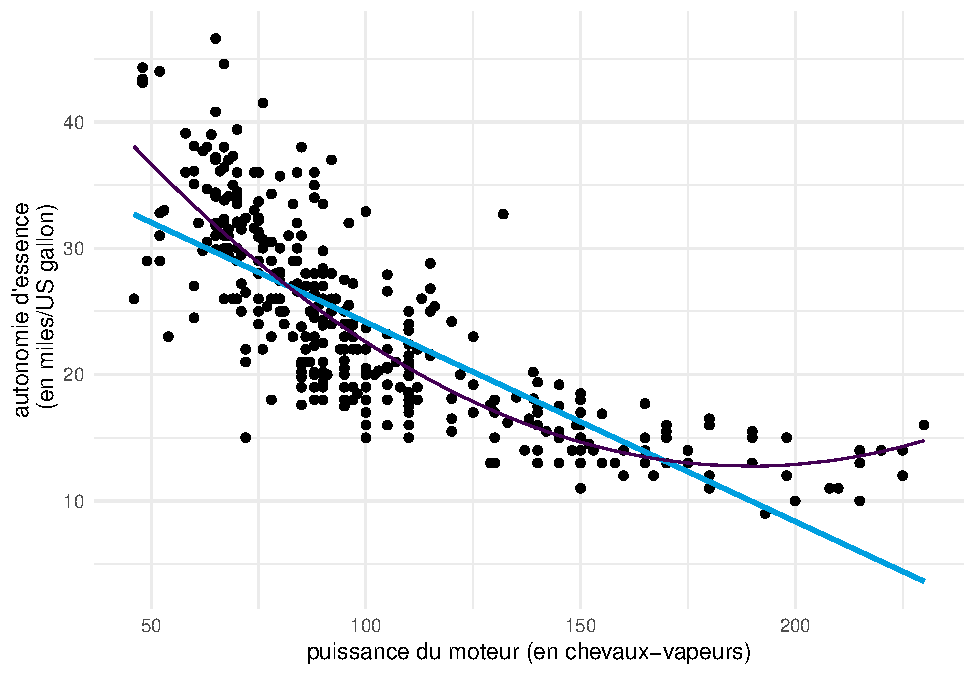
\includegraphics[width=0.7\linewidth]{MATH60604_Modelisation_statistique_files/figure-latex/autoquad2d-1} 

}

\caption{Modèle de régression avec terme quadratique pour la puissance}\label{fig:autoquad2d}
\end{figure}

À vue d'oeil, l'ajustement est meilleur pour le modèle quadratique: nous verrons plus tard à l'aide de test si cette observation est vérifiée statistiquement.
On voit aussi dans la Figure \ref{fig:autoquad2d} que l'autonomie d'essence décroît rapidement quand la puissance croît entre \(0\) et \(189.35\), mais semble remonter légèrement par la suite pour les voitures qui un moteur de plus de 200 chevaux-vapeurs, ce que le modèle quadratique capture. Prenez garde en revanche à l'extrapolation là où vous n'avez pas de données (comme l'illustre remarquablement bien \href{https://livefreeordichotomize.com/2020/05/05/model-detective/}{le modèle cubique de Hassett pour le nombre de cas quotidiens de coronavirus}).

La représentation graphique du modèle polynomial de degré 2 présenté dans la Figure \ref{fig:autoquad2d} peut sembler contre-intuitive, mais c'est une projection en 2D d'un plan 3D de coordonnées \(\beta_0 + \beta_1x-y +\beta_2z =0\), où \(x=\texttt{puissance}\), \(z=\texttt{puissance}^2\) et \(y=\texttt{autonomie}\). La physique et le bon-sens imposent la contrainte \(z = x^2\), et donc les valeurs ajustées vivent sur une courbe dans un sous-espace du plan ajusté, représenté en gris dans la Figure \ref{fig:hyperplan}.

\begin{figure}

{\centering 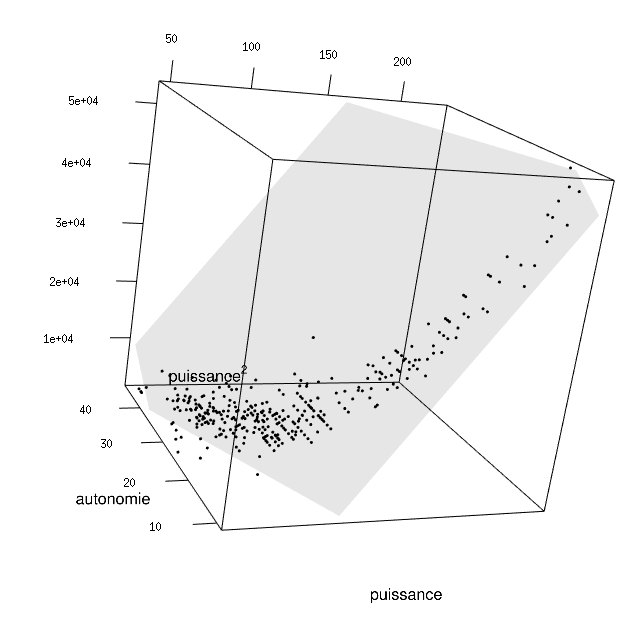
\includegraphics[width=0.7\linewidth]{images/hyperplan_auto} 

}

\caption{Représentation graphique 3D du modèle de régression linéaire pour les données $    exttt{automobile}$.}\label{fig:hyperplan}
\end{figure}

\begin{remark}[Utilisation de bases polynomiales pour les effets nonlinéaires]
\iffalse{} {Remarque (Utilisation de bases polynomiales pour les effets nonlinéaires). } \fi{}Règle générale, on utilise des représentations flexibles (bases de splines) plutôt que des modèles polynomiaux pour le lissage si la relation entre une variable \(Y\) et une variable explicative \(\mathrm{X}\) est nonlinéaire. Une compréhension de la physique du système à l'étude, ou bien un modèle théorique permet aussi de guider le choix des fonctions (non)linéaires à utiliser.
\end{remark}

Le coefficient \(\beta_j\) est la contribution
\emph{marginale} de \(\mathrm{X}_j\) quand les autres covariables sont incluses dans le modèle. On peut représenter graphiquement cet effet en projetant les vecteurs \(Y\) et \(\mathrm{X}_j\) dans le complément orthogonal de \(\mathbf{X}_{-j}\). Le diagramme de régression partielle est un diagnostic graphique qui illustre la valeur ajoutée de \(\mathrm{X}_j\): il montre en ordonnée (axe des \(y\)), les résidus du modèle de régression pour \(Y\) avec toutes les variables explicatives sauf \(\mathrm{X}_j\), et en abcisse (axe des \(x\)), les résidus de la régression de \(\mathrm{X}_j\) sur les autres variables explicatives. La droite de régression qui satisfait le critère des moindre carrés pour ce nuage de points passe par (\(0,0\)) et sa pente est \(\hat{\beta}_j\). Ce diagnostic est particulièrement utile pour détecter l'impact de valeurs aberrantes ou la colinéarité.

\begin{example}[Inéquité salariale dans un collège américain]
\protect\hypertarget{exm:inequite-salariale}{}{\label{exm:inequite-salariale} \iffalse (Inéquité salariale dans un collège américain) \fi{} }On considère les données \texttt{college} et un modèle de régression qui inclut le sexe, l'échelon académique, le nombre d'années de service et le domaine d'expertise (appliquée ou théorique).
\end{example}

Si on multiplie le salaire par mille, le modèle linéaire postulé s'écrit
\begin{align*}
\texttt{salaire} \times 1000 &= \beta_0 + \beta_1 \texttt{sexe}_{\texttt{femme}} +\beta_2 \texttt{domaine}_{\texttt{theorique}} \\&\quad +\beta_3 \texttt{echelon}_{\texttt{aggrege}}
+\beta_4 \texttt{echelon}_{\texttt{titulaire}}  +\beta_5 \texttt{service} + \varepsilon.
\end{align*}

\begin{table}

\caption{\label{tab:collegecoefs}Estimés des coefficients du modèle linéaire pour les données $\texttt{college}$ (en dollars USD, arrondis à l'unité).}
\centering
\begin{tabular}[t]{rrrrrr}
\toprule
$\widehat{\beta}_0$ & $\widehat{\beta}_1$ & $\widehat{\beta}_2$ & $\widehat{\beta}_3$ & $\widehat{\beta}_4$ & $\widehat{\beta}_5$\\
\midrule
86596 & -4771 & -13473 & 14560 & 49160 & -89\\
\bottomrule
\end{tabular}
\end{table}

L'interprétation des coefficients est la suivante:

\begin{itemize}
\tightlist
\item
  L'ordonnée à l'origine \(\beta_0\) correspond au salaire moyen d'un professeur adjoint (un homme) qui vient de compléter ses études et qui travaille dans un domaine appliqué: on estime ce salaire à \(\widehat{\beta}_0=86596\) dollars.
\item
  toutes choses étant égales par ailleurs (même domaine, échelon et années depuis le dernier diplôme), l'écart de salaire entre un homme et un femme est estimé à \(\widehat{\beta}_1=-4771\) dollars.
\item
  \emph{ceteris paribus}, un(e) professeur(e) qui oeuvre dans un domaine théorique gagne \(\beta_2\) dollars de plus qu'une personne du même sexe dans un domaine appliqué; on estime cette différence à \(-13473\) dollars.
\item
  \emph{ceteris paribus}, la différence moyenne de salaire entre professeurs adjoints et aggrégés est estimée à \(\widehat{\beta}_3=14560\) dollars.
\item
  \emph{ceteris paribus}, la différence moyenne de salaire entre professeurs adjoints et titulaires est de \(\widehat{\beta}_4=49160\) dollars.
\item
  au sein d'un même échelon, chaque année supplémentaire de service mène à une augmentation de salaire annuelle moyenne de \(\widehat{\beta}_5=-89\) dollars.
\end{itemize}

On voit que les femmes sont moins payées que les hommes: reste à savoir si cette différence est statistiquement significative. L'estimé de la surprime annuelle due à l'expérience est négative, un résultat contre-intuitif au vu de la Figure \ref{fig:droitenuage} qui montrait une augmentation notable du salaire avec les années. Cette représentation graphique est trompeuse: la Figure \ref{fig:edacollege} montrait l'impact important de l'échelon académique. Une fois tous les autres facteurs pris en compte, le nombre d'années de service n'apporte que peu d'information au modèle et le diagramme de régression partielle de la Figure \ref{fig:avplotcollege} illustre l'absence de corrélation entre salaire et la partie non expliquée par les autres covariables; les gens avec un grand nombre d'années de service sont moins payés que certains de leurs collègues, ce qui explique la pente négative.

\begin{figure}

{\centering 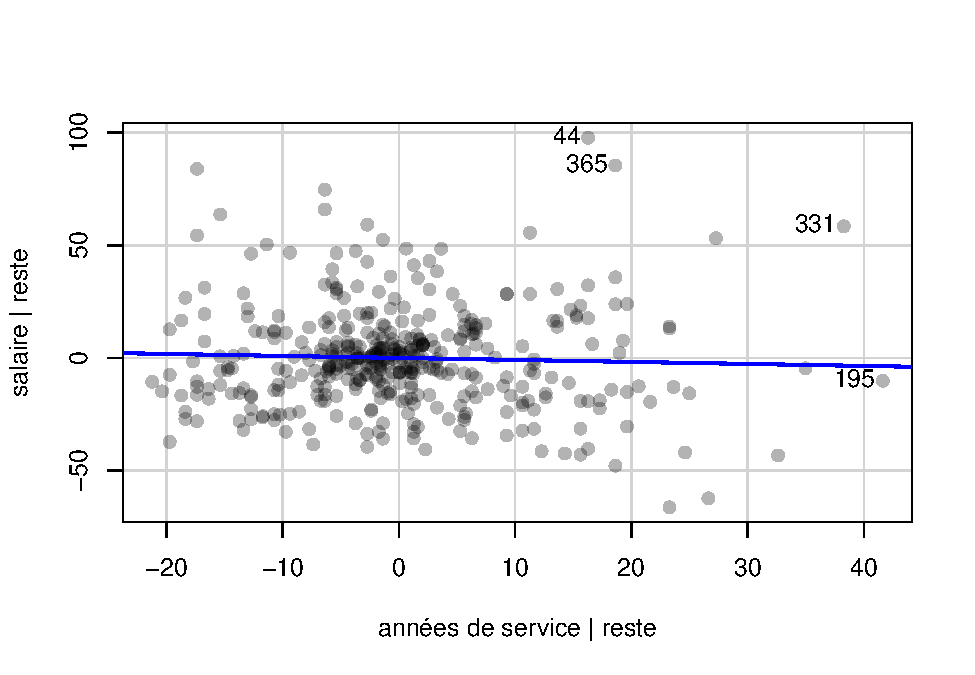
\includegraphics[width=0.7\linewidth]{MATH60604_Modelisation_statistique_files/figure-latex/avplotcollege-1} 

}

\caption{Diagramme de régression partielle pour les années de service dans le modèle de régression linéaire pour les données $\texttt{college}$.}\label{fig:avplotcollege}
\end{figure}

\hypertarget{vraisemblance}{%
\section{Inférence basée sur la vraisemblance}\label{vraisemblance}}

\hypertarget{modeles-lineaires-generalises}{%
\section{Modèles linéaires généralisés}\label{modeles-lineaires-generalises}}

\hypertarget{donnees-correlees-longitudinales}{%
\section{Données corrélées et longitudinales}\label{donnees-correlees-longitudinales}}

\hypertarget{modeles-lineaires-mixtes}{%
\section{Modèles linéaires mixtes}\label{modeles-lineaires-mixtes}}

\hypertarget{comparaison-de-moduxe8les}{%
\subsection{Comparaison de modèles}\label{comparaison-de-moduxe8les}}

Cette brève discussion traite de méthodes de comparaisons de modèles selon différents scénarios d'intérêt.
En particulier, puisque la plupart des logiciels promeuvent l'utilisation du critère de vraisemblance restreinte (REML) par défaut pour l'ajustement de modèles mixtes, il convient de porter une attention spéciale aux tests que l'on réalise.

En ajustant un modèle avec la méthode REML, on élimine la contribution de la moyenne de la vraisemblance. Cela permet d'obtenir des estimateurs des paramètres de variance \(\boldsymbol{\psi}\) qui sont moins biaisés, mais cette fonction objective ne permet pas de comparer des modèles qui ont une matrice de modèle \(\mathbf{X}\) différente.

On préfère si possible les tests d'hypothèse (rapport de vraisemblance) aux critères d'informations pour la sélection de modèle. Les tests d'hypothèse requièrent la comparaison de deux modèles \textbf{emboîtés}: c'est le cas si on peut obtenir en imposant des contraintes sur \textbf{un} des modèles le second.

\begin{itemize}
\tightlist
\item
  Test du rapport de vraisemblance, méthode du maximum de vraisemblance restreint (REML): modèles emboîtés, même modèle pour la moyenne. Par exemple, tester si le modèle d'équicorrélation \(\mathsf{CS}\) est une simplification adéquate du modèle non-structure \(\mathsf{UN}\).
\item
  Test du rapport de vraisemblance, méthode du maximum de vraisemblance: modèles emboîtés (pas d'autre contrainte). Par exemple, dans un modèle linéaire avec erreurs autorégressives, tester si l'effet de la variable \(\mathrm{X}_j\) est nul sachant le reste et si les erreurs sont indépendantes, soit \(\mathscr{H}_0: \beta_j=0\), \(\mathscr{H}_0: \rho=0\), ou encore \(\mathscr{H}_0: \beta_j=\rho=0\).
\end{itemize}

Si on veut comparer des modèles non-emboîtés, on doit se rabattre sur la performance prédictive ou les critères d'information. Dans ce dernier cas, il faut que les deux modèles aient les même variables réponse. Si on utilise des fonctions de vraisemblance différentes, il faut aussi s'assurer que notre logiciel calcule les constantes de normalisation pour s'assurer que la comparaison soit valide.

\begin{itemize}
\tightlist
\item
  Par exemple, comparer un modèle linéaire avec erreurs autorégressives \(\mathsf{AR}(1)\) versus un modèle avec un effet aléatoire sur la pente.
\end{itemize}

La seule comparaison de modèle emboîtés que je vous déconseille de faire à l'aide de tests d'hypothèse est celle dans lequel la comparaison entre les deux modèles implique de contraindre des paramètres positifs à zéro (éliminer un effet aléatoire revient à fixer sa variance à zéro). Ce faisant, on se trouve avec un cas où la valeur du paramètre est sur la bordure de l'espace des valeurs admissible. Ce cas limite donne une loi nulle différente de la loi \(\chi^2\) usuelle. Bien que la statistique de test soit calculable et correcte, l'approximation de la loi de référence est compliquée à dériver et de mauvaise qualité.

\begin{itemize}
\tightlist
\item
  Exemple de scénarios: regarder dans un modèle avec \(\boldsymbol{b} \sim \mathsf{No}_2(\boldsymbol{0}_2, \boldsymbol{\Omega})\), où \(b_1\) est une ordonnée à l'origine aléatoire et \(b_2\) une pente aléatoire. Tester si la pente aléatoire est nécessaire revient à tester \(\mathscr{H}_0: \omega_{22}=0\), et comme le paramètre de variance est positif, ce test n'est pas régulier.
\end{itemize}

\hypertarget{survie}{%
\section{Analyse de survie}\label{survie}}

\hypertarget{appendix-annexe}{%
\appendix}


\hypertarget{complement}{%
\section{Compléments mathématiques}\label{complement}}

\hypertarget{population-echantillon}{%
\subsection{Population et échantillons}\label{population-echantillon}}

Ce qui différencie la statistique des autres sciences est la prise en compte de l'incertitude et de la notion d'aléatoire. Règle générale, on cherche à estimer une caractéristique d'une population définie à l'aide d'un échantillon (un sous-groupe de la population) de taille restreinte.

La \textbf{population d'intérêt} est une collection d'individus formant la matière première d'une étude statistique. Par exemple, pour l'Enquête sur la population active (EPA) de Statistique Canada, « la population cible comprend la population canadienne civile non institutionnalisée de 15 ans et plus ». Même si on faisait un recensement et qu'on interrogeait tous les membres de la population cible, la caractéristique d'intérêt peut varier selon le moment de la collecte; une personne peut trouver un emploi, quitter le marché du travail ou encore se retrouver au chômage. Cela explique la variabilité intrinsèque.

En général, on se base sur un \textbf{échantillon} pour obtenir de l'information. L'\textbf{inférence statistique} vise à tirer des conclusions, pour toute la population, en utilisant seulement l'information contenue dans l'échantillon et en tenant compte des sources de variabilité. Le sondeur George Gallup (traduction libre) a fait cette merveilleuse analogie entre échantillon et population:

\begin{quote}
«Il n'est pas nécessaire de manger un bol complet de soupe pour savoir si elle est trop salé; pour autant qu'elle ait été bien brassée, une cuillère suffit.»
\end{quote}

Un \textbf{échantillon} est un sous-groupe d'individus tiré aléatoirement de la population. La création de plans d'enquête est un sujet complexe et des cours entiers d'échantillonnage y sont consacrés. Même si on ne collectera pas de données, il convient de noter la condition essentielle pour pouvoir tirer des conclusions fiables à partir d'un échantillon: ce dernier doit être représentatif de la population étudiée, en ce sens que sa composition doit être similaire à celle de la population. On doit ainsi éviter les biais de sélection, notamment les échantillons de commodité qui consistent en une sélection d'amis et de connaissances.

Si notre échantillon est \textbf{aléatoire}, notre mesure d'une caractéristique d'intérêt le sera également et la conclusion de notre procédure de test variera d'un échantillon à l'autre. Plus la taille de ce dernier est grande, plus on obtiendra une mesure précise de la quantité d'intérêt. L'exemple suivant illustre pourquoi le choix de l'échantillon est important.

\begin{example}
\protect\hypertarget{exm:Galluppoll}{}{\label{exm:Galluppoll} }
Désireuse de prédire le résultat de l'élection présidentielle américaine de 1936, la revue \emph{Literary Digest} a sondé 10 millions d'électeurs par la poste, dont 2.4 millions ont répondu au sondage en donnant une nette avance au candidat républicain Alf Landon (57\%) face au président sortant Franklin D. Roosevelt (43\%). Ce dernier a néanmoins remporté l'élection avec 62\% des suffrages, une erreur de prédiction de 19\%. Le plan d'échantillonnage avait été conçu en utilisant des bottins téléphoniques, des enregistrements d'automobiles et des listes de membres de clubs privés, etc.: \href{https://www.jstor.org/stable/2749114}{la non-réponse différentielle et un échantillon biaisé vers les classes supérieures sont en grande partie responsable de cette erreur.}

Gallup avait de son côté correctement prédit la victoire de Roosevelt en utilisant un échantillon aléatoire de (seulement) 50 000 électeurs. \href{https://medium.com/@ozanozbey/how-not-to-sample-11579793dac}{L'histoire complète (en anglais).}
\end{example}

\hypertarget{variable-aleatoire}{%
\subsection{Variables aléatoires}\label{variable-aleatoire}}

Suppsons qu'on cherche à décrire le comportement d'un phénomène aléatoire. Pour ce faire, on cherche à décrire l'ensemble des valeurs possibles et leur probabilité/fréquence relative au sein de la population: ces dernières sont encodées dans la loi de la variable aléatoire.

On fera la distinction entre deux cas de figure: quand le phénomène prend des valeurs finies, comme par exemple un événement binaire (achat/non-achat d'un produit) ou un continuum de valeurs (par exemple, le prix d'un item). On dénote les variables aléatoires par des lettres majuscules: par exemple, \(Y \sim \mathsf{No}(\mu, \sigma^2)\) indique que \(Y\) suit une loi normale de paramètres \(\mu\) et \(\sigma\), qui représentent respectivement l'espérance et l'écart-type de \(Y\).

La fonction de répartition \(F(y)\) donne la probabilité cumulative qu'un événement n'excède pas une variable donnée, \(F(y) = \mathsf{Pr}(Y \leq y)\).

Si la variable \(Y\) prend des valeurs discrètes, alors on utilise la fonction de masse \(f(y)=\mathsf{Pr}(Y=y)\) qui donne la probabilité pour chacune des valeurs de \(y\).
Si la variable \(Y\) est continue, aucune valeur numérique de \(y\) n'a de probabilité non-nulle; la densité sert à estimer la probabilité que la variable \(Y\) appartienne à un ensemble \(B\), via \(\mathsf{Pr}(Y \in B) = \int_B f(y) \mathrm{d} y\); la fonction de répartition est ainsi \(F(y) = \int_{-\infty}^y f(x) \mathrm{d} x\).

\begin{figure}

{\centering 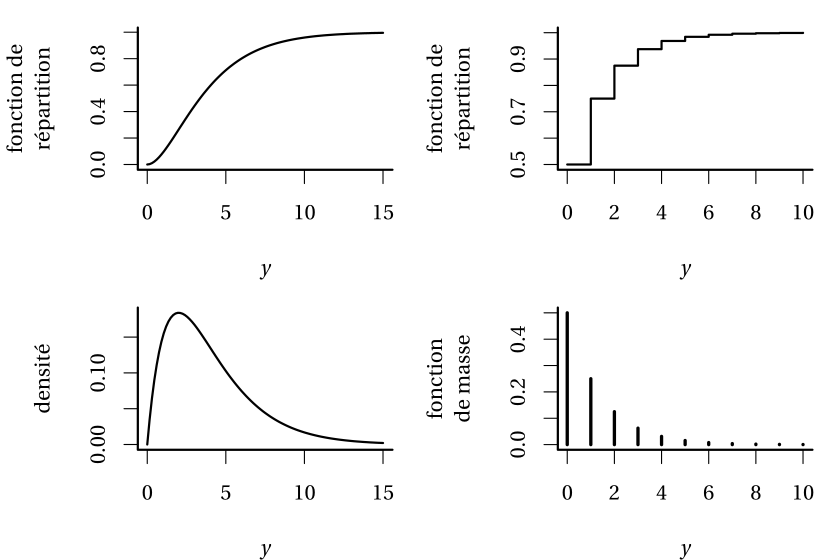
\includegraphics[width=0.7\linewidth]{images/02-ttest-DF_illustration_fr} 

}

\caption{Fonctions de répartition (panneau supérieur) et fonctions de densité et de masse (panneau inférieur) pour une loi continue (gauche) et discrète (droite).}\label{fig:distributions}
\end{figure}

\hypertarget{moments}{%
\subsubsection{Moments}\label{moments}}

Un premier cours de statistique débute souvent par la présentation de statistiques descriptives comme la moyenne et l'écart-type. Ce sont des estimateurs des moments (centrés), qui caractérisent la loi du phénomène d'intérêt. Dans le cas de la loi normale unidimensionnelle, qui a deux paramètres, l'espérance et la variance caractérisent complètement le modèle.

Soit \(Y\) une variable aléatoire de fonction de densité (ou de masse) \(f(x)\). Cette fonction est non-négative et satisfait \(\int_{\mathbb{R}} f(x) \mathrm{d}x=1\): elle décrit la probabilité d'obtenir un résultat dans un ensemble donné des réels \(\mathbb{R}\).

On définit l'espérance d'une variable aléatoire \(Y\) comme \[\mathsf{E}(Y)=\int_{\mathbb{R}} x f(x) \mathrm{d} x.\]
L'espérance est la « moyenne théorique» : dans le cas discret, \(\mu = \mathsf{E}(Y)=\sum_{x \in \mathcal{X}} x \mathsf{Pr}(X=x)\), où \(\mathcal{X}\) représente le support de la loi, à savoir les valeurs qui ont une probabilité non-nulle. Plus généralement, l'espérance d'une fonction \(g(x)\) pour une variable aléatoire \(Y\) est simplement l'intégrale de \(g(x)\) pondérée par la densité \(f(x)\). De même, si l'intégrale est convergente, la variance est
\[\mathsf{Va}(Y)=\mathsf{E}\{Y-\mathsf{E}(Y)\}^2 \equiv \int_{\mathbb{R}} (x-\mu)^2 f(x) \mathrm{d} x.\]

Un estimateur \(\hat{\theta}\) pour un paramètre \(\theta\) est sans biais si son biais \(\mathsf{biais}(\hat{\theta})=\mathsf{E}(\hat{\theta})- \theta\) est nul.
L'estimateur sans biais de l'espérance de \(Y\) est \(\overline{Y}_n = n^{-1} \sum_{i=1}^n Y_i\) et celui de la variance \(S_n = (n-1)^{-1} \sum_{i=1}^n (Y_i-\overline{Y})^2\). Un estimateur sans biais est souhaitable, mais pas toujours optimal. Quelquefois, il n'existe pas d'estimateur non-biaisé!

Souvent, on cherche à balancer le biais et la variance: rappelez-vous qu'un estimateur est une variable aléatoire (étant une fonction de variables aléatoires) et qu'il est lui-même variable: même s'il est sans biais, la valeur numérique obtenue fluctuera d'un échantillon à l'autre. On peut chercher un estimateur qui minimise l'erreur moyenne quadratique, \[\mathsf{EMQ}(\hat{\theta}) = \mathsf{E}\{(\hat{\theta}-\theta)^2\}=\mathsf{Va}(\hat{\theta}) + \{\mathsf{E}(\hat{\theta})\}^2.\]
C'est donc un compromis entre le carré du biais et la variance de l'estimateur.
La plupart des estimateurs que nous considérerons dans le cadre du cours sont
des estimateurs du maximum de vraisemblance. Ces derniers sont asymptotiquement efficaces, c'est-à-dire qu'ils minimisent l'erreur moyenne quadratique parmi tous les estimateurs possibles quand la taille de l'échantillon est suffisamment grande. Ils ont également d'autre propriétés qui les rendent attractifs comme choix par défaut pour l'estimation.

\hypertarget{distributions}{%
\subsubsection{Distributions}\label{distributions}}

Plusieurs lois aléatoires décrivent des phénomènes physiques simples et ont donc une justification empirique; on revisite les distributions les plus fréquemment couvertes.

\begin{example}[Loi de Bernoulli]
\protect\hypertarget{exm:loibern}{}{\label{exm:loibern} \iffalse (Loi de Bernoulli) \fi{} }On considère un phénomène binaire, comme le lancer d'une pièce de monnaie (pile/face). De manière générale, on associe les deux possibilités à succès/échec et on suppose que la probabilité de succès est \(\pi\). Par convention, on représente les échecs (non) par des zéros et les réussites (oui) par des uns. Donc, si la variable \(Y\) vaut \(0\) ou \(1\), alors \(\mathsf{Pr}(Y=1)=\pi\) et \(\mathsf{Pr}(Y=0)=1-\pi\) (complémentaire). La fonction de masse de la \href{https://fr.wikipedia.org/wiki/Loi_de_Bernoulli}{loi Bernoulli} s'écrit de façon plus compacte
\begin{align*}
\mathsf{Pr}(Y=y) = \pi^y (1-\pi)^{1-y}, \quad y=0, 1.
\end{align*}

Un calcul rapide montre que \(\mathsf{E}(Y)=\pi\) et \(\mathsf{Va}(Y)=\pi(1-\pi)\).
Voici quelques exemples de questions de recherches comprenant une variable réponse binaire:

\begin{itemize}
\tightlist
\item
  est-ce qu'un client potentiel a répondu favorablement à une offre
  promotionnelle?
\item
  est-ce qu'un client est satisfait du service après-vente?
\item
  est-ce qu'une firme va faire faillite au cours des trois prochaines années?
\item
  est-ce qu'un participant à une étude réussit une tâche?
\end{itemize}
\end{example}

\begin{example}[Loi binomiale]
\protect\hypertarget{exm:loibinom}{}{\label{exm:loibinom} \iffalse (Loi binomiale) \fi{} }Si les données représentent la somme d'événements Bernoulli indépendants, la loi du nombre de réussites \(Y\) pour un nombre d'essais donné \(m\) est dite \href{https://fr.wikipedia.org/wiki/Loi_binomiale}{binomiale}, dénotée \(\mathsf{Bin}(m, \pi)\); sa fonction de masse est
\begin{align*}
\mathsf{Pr}(Y=y) = \binom{m}{y}\pi^y (1-\pi)^{1-y}, \quad y=0, 1.
\end{align*}
La vraisemblance pour un échantillon de la loi binomiale est (à constante de normalisation près qui ne dépend pas de \(\pi\)) la même que pour un échantillon aléatoire de \(m\) variables Bernoulli indépendantes. L'espérance d'une variable binomiale est \(\mathsf{E}(Y)=m\pi\) et la variance \(\mathsf{Va}(Y)=m\pi(1-\pi)\).

On peut ainsi considérer le nombre de personnes qui ont obtenu leur permis de conduire parmi \(m\) candidat(e)s ou le nombre de clients sur \(m\) qui ont passé une commande de plus de 10\$ dans un magasin.
\end{example}

Plus généralement, on peut considérer des variables de dénombrement qui prennent des valeurs entières. Parmi les exemples de questions de recherches comprenant une variable réponse de dénombrement:

\begin{itemize}
\tightlist
\item
  le nombre de réclamations faites par un client d'une compagnie d'assurance
  au cours d'une année.
\item
  le nombre d'achats effectués par un client depuis un mois.
\item
  le nombre de tâches réussies par un participant lors d'une étude.
\end{itemize}

\begin{example}[Loi géométrique]
\protect\hypertarget{exm:loigeom}{}{\label{exm:loigeom} \iffalse (Loi géométrique) \fi{} }La \href{https://fr.wikipedia.org/wiki/Loi_g\%C3\%A9om\%C3\%A9trique}{loi géométrique} décrit le comportement du nombre d'essais Bernoulli de probabilité de succès \(\pi\) nécessaires avant l'obtention d'un premier succès. La fonction de masse de \(Y \sim \mathsf{Geo}(\pi)\) est
\begin{align*}
\mathsf{Pr}(Y=y) = \pi (1-\pi)^{y-1}, \quad y=1,2, \ldots
\end{align*}

Par exemple, on pourrait modéliser le nombre de visites d'une maison en vente avant une première offre d'achat à l'aide d'une variable géométrique.
\end{example}

\begin{example}[Loi de Poisson]
\protect\hypertarget{exm:loipoisson}{}{\label{exm:loipoisson} \iffalse (Loi de Poisson) \fi{} }Si la probabilité d'un événement Bernoulli est petite (succès rare) dans le sens où \(m\pi \to \lambda\) quand le nombre d'essais \(m\) augmente, alors le nombre de succès suit une loi de Poisson de fonction de masse
\begin{align*}
\mathsf{Pr}(Y=y) = \frac{\exp(-\lambda)\lambda^y}{\Gamma(y+1)}, \quad y=0, 1, 2, \ldots
\end{align*}
où \(\Gamma(\cdot)\) dénote la fonction gamma. Le paramètre \(\lambda\) de la loi de Poisson représente à la fois l'espérance et la variance de la variable, c'est-à-dire que \(\mathsf{E}(Y)=\mathsf{Va}(Y)=\lambda\).
\end{example}

\begin{example}[Loi binomiale négative]
\protect\hypertarget{exm:loibinneg}{}{\label{exm:loibinneg} \iffalse (Loi binomiale négative) \fi{} }On considère une série d'essais Bernoulli de probabilité de succès \(\pi\) jusqu'à l'obtention de \(m\) succès. Soit \(Y\), le nombre d'échecs: puisque la dernière réalisation doit forcément être un succès, mais que l'ordre des succès/échecs précédents n'importe pas, la fonction de masse est
\begin{align*}
\mathsf{Pr}(Y=y)= \binom{m-1+y}{y} \pi^m (1-\pi)^{y}.
\end{align*}

La loi binomiale négative apparaît également si on considère la loi non-conditionnelle du modèle hiérarchique gamma-Poisson, dans lequel on suppose que le paramètre de la moyenne de la loi Poisson est aussi aléatoire, c'est-à-dire \(Y \mid \Lambda=\lambda \sim \mathsf{Po}(\lambda)\) et \(\Lambda\) suit une loi gamma de paramètre de forme \(r\) et de paramètre d'échelle \(\theta\), dont la densité est \[f(x) = \theta^{-r}x^{r-1}\exp(-x/\theta)/\Gamma(r).\] Le nombre d'événements suit alors une loi binomiale négative.

La paramétrisation la plus courante pour la modélisation est légèrement différente: on utilise la fonction de masse est
\begin{align*}
\mathsf{Pr}(Y=y)=\frac{\Gamma(y+r)}{\Gamma(y+1)\Gamma(r)} \left(\frac{r}{r + \mu} \right)^{r} \left(\frac{\mu}{r+\mu}\right)^y, y=0, 1, \ldots, \mu,r >0,
\end{align*}
où \(\Gamma\) dénote la fonction gamma. À noter que le paramètre \(r>0\) n'est plus nécessairement entier. La moyenne théorique et la variance sont
\(\mathsf{E}(Y)=\mu\) et \(\mathsf{Va}(Y)=\mu+k\mu^2\), où \(k=1/r\). La variance d'une variable binomiale négative est \emph{supérieure} à sa moyenne et le modèle est utilisé comme alternative à la loi de Poisson pour modéliser la surdispersion.
\end{example}

\hypertarget{diagramme-qq}{%
\subsubsection{Diagrammes quantiles-quantiles}\label{diagramme-qq}}

Si on ajuste un modèle à des données, il convient de vérifier la qualité de l'ajustement et l'adéquation du modèle, par exemple graphiquement. Le diagramme quantile-quantile sert à vérifier l'adéquation du modèle et découle du constat suivant: si \(Y\) est une variable aléatoire continue et \(F\) sa fonction de répartition, alors l'application \(F(Y) \sim \mathsf{U}(0,1)\). De la même façon, appliquer la fonction quantile à une variable uniforme permet de simuler de la loi \(F\), et donc \(F^{-1}(U)\). Supposons un échantillon de taille \(n\) de variables uniformes. On peut démontrer que les statistiques d'ordre \(U_{(1)} \leq \cdots \leq U_{(n)}\) ont une loi marginale Beta: et \(U_{(k)} \sim \mathsf{Beta}(k, n+1-k)\) d'espérance \(k/(n+1)\).

Les paramètres de la loi \(F\) sont inconnus, mais on peut obtenir un estimateur \(\widehat{F}\) et appliquer la transformation inverse pour obtenir une variable approximativement uniforme. Un diagramme quantile-quantile représente les données en fonction des moments des statistiques d'ordre transformées

\begin{itemize}
\tightlist
\item
  sur l'axe des abscisses, les quantiles théoriques \(\widehat{F}^{-1}\{\mathrm{rang}(Y_i)/(n+1)\}\)
\item
  sur l'axe des ordonnées, les quantiles empiriques \(Y_i\)
\end{itemize}

Si le modèle est adéquat, les valeurs ordonnées devraient suivre une droite de pente unitaire qui passe par l'origine. L'oeil humain a de la difficulté à juger de la qualité de l'adéquation en regardant une droite, aussi est-il préférable de soustraire cette pente pour faciliter l'interprétation (une méthode proposée par Tukey, mais faire attention à l'échelle!) Les données de la Figure \ref{fig:diagrammeqq2} montrent ces deux représentations sur des mêmes données simulées d'une loi normale standard.

\begin{figure}

{\centering 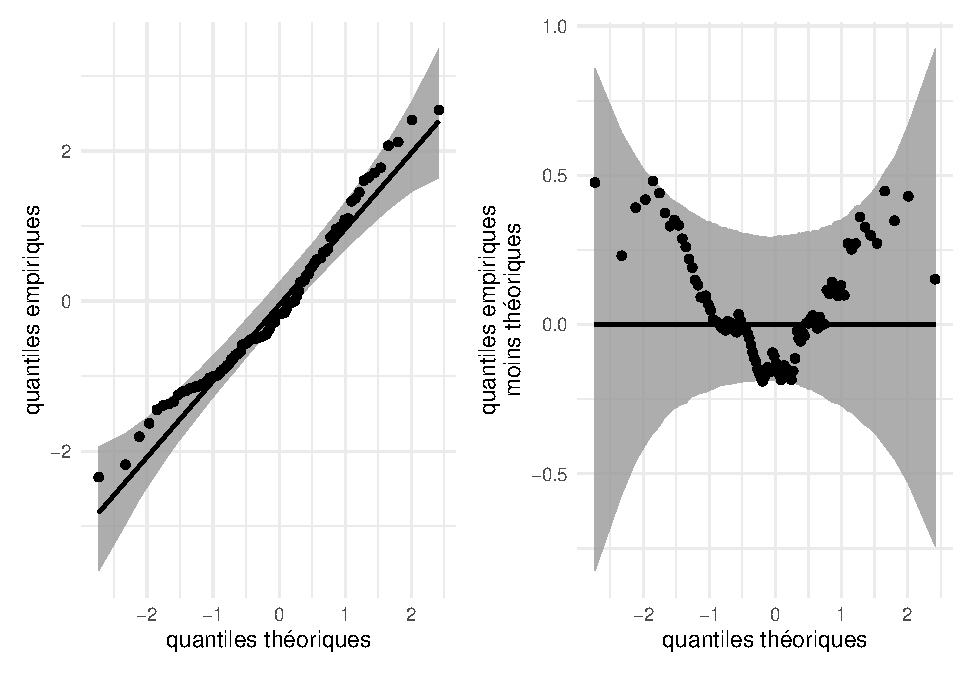
\includegraphics[width=0.7\linewidth]{MATH60604_Modelisation_statistique_files/figure-latex/diagrammeqq2-1} 

}

\caption{Diagramme quantile-quantile normal (gauche) et représentation de Tukey du même diagramme (en soustrayant la traîne)}\label{fig:diagrammeqq2}
\end{figure}

Même si on connaissait exactement la loi aléatoire des données, la variabilité intrinsèque à l'échantillon fait en sorte que des déviations qui semblent significatives et anormales à l'oeil de l'analyste sont en fait compatibles avec le modèle: un simple estimé ponctuel sans mesure d'incertitude ne permet donc pas facilement de voir ce qui est plausible ou pas. On va donc idéalement ajouter un intervalle de confiance (approximatif) ponctuel ou conjoint au diagramme.

Pour obtenir l'intervalle de confiance approximatif, la méthode la plus simple est par simulation (autoamorçage paramétrique), en répétant \(B\) fois les étapes suivantes

\begin{enumerate}
\def\labelenumi{\arabic{enumi}.}
\tightlist
\item
  simuler un échantillon \(\{Y^{(b)}_{i}\} (i=1,\ldots, n)\) du modèle \(\widehat{F}\)
\item
  estimer les paramètres du modèle \(F\) pour obtenir \(\widehat{F}_{(b)}\)
\item
  calculer et stocker les positions \(\widehat{F}^{-1}_{(b)}\{i/(n+1)\}\).
\end{enumerate}

Le résultat de cette opération sera une matrice \(n \times B\) de données simulées; on obtient un intervalle de confiance symmétrique en conservant le quantile \(\alpha/2\) et \(1-\alpha/2\) de chaque ligne. Le nombre de simulation \(B\) devrait être large (typiquement 999 ou davantage) et être choisi de manière à ce que \(B/alpha\) soit un entier.

Pour l'intervalle de confiance ponctuel, chaque valeur représente une statistique et donc individuellement, la probabilité qu'une statistique d'ordre sorte de l'intervalle de confiance est \(\alpha\). En revanche, les statistiques d'ordres ne sont pas indépendantes et sont qui est plus ordonnées, ce qui fait qu'un point hors de l'intervalle risque de n'être pas isolé. {[}Il est aussi possible d'obtenir par autoamorçage un intervalle de confiance (approximatif) conjoint, pour lequel une valeur sort de l'intervalle \(100(1-\alpha)\)\% du temps; \href{https://lbelzile.github.io/lineaRmodels/qqplot.html}{voir à ce sujet mes notes de cours Section 4.4.3 (en anglais)}. Les intervalles présentés dans la Figure \ref{fig:diagrammeqq2} sont ponctuels. La variabilité des statistiques d'ordre uniformes est plus grande à mesure qu'on s'éloigne de 1/2, mais celles des variables transformées dépend de \(F\).

\hypertarget{loi-grands-nombres}{%
\subsection{Loi des grands nombres}\label{loi-grands-nombres}}

Un estimateur est dit \textbf{convergent} si la valeur obtenue à mesure que la taille de l'échantillon augmente s'approche de la vraie valeur que l'on cherche à estimer. Mathématiquement parlant, un estimateur est dit convergent s'il converge en probabilité, ou \(\hat{\theta} \stackrel{\mathsf{Pr}}{\to} \theta\): en langage commun, la probabilité que la différence entre \(\hat{\theta}\) et \(\theta\) diffèrent est négligeable quand \(n\) est grand.

La condition \emph{a minima} pour le choix d'un estimateur est donc la convergence: plus on récolte d'information, plus notre estimateur devrait s'approcher de la valeur qu'on tente d'estimer.

La loi des grands nombres établit que la moyenne empirique de \(n\) observations indépendantes de même espérance, \(\overline{Y}_n\), tend vers l'espérance commune des variables \(\mu\), où \(\overline{Y}_n \rightarrow \mu\). En gros, ce résultat nous dit que l'on réussit à approximer de mieux en mieux la quantité d'intérêt quand la taille de l'échantillon (et donc la quantité d'information disponible sur le paramètre) augmente. La loi des grands nombres est très utile dans les expériences Monte Carlo: on peut ainsi approximer par simulation la moyenne d'une fonction \(g(x)\) de variables aléatoires en simulant de façon répétée des variables \(Y\) indépendantes et identiquement distribuées et en prenant la moyenne empirique \(n^{-1} \sum_{i=1}^n g(Y_i)\).

Si la loi des grands nombres nous renseigne sur le comportement limite ponctuel, il ne nous donne aucune information sur la variabilité de notre estimé de la moyenne et la vitesse à laquelle on s'approche de la vraie valeur du paramètre.

\hypertarget{TCL}{%
\subsection{Théorème central limite}\label{TCL}}

Le théorème central limite dit que, pour un échantillon aléatoire de taille \(n\) dont les observations sont indépendantes et tirées d'une loi quelconque d'espérance \(\mu\) et de variance finie \(\sigma^2\), alors la moyenne empirique tend non seulement vers \(\mu\), mais à une vitesse précise:

\begin{itemize}
\tightlist
\item
  l'estimateur \(\overline{Y}\) sera centré autour de \(\mu\),
\item
  l'erreur-type sera de \(\sigma/\sqrt{n}\); le taux de convergence est donc de \(\sqrt{n}\). Ainsi, pour un échantillon de taille 100, l'erreur-type de la moyenne empirique sera 10 fois moindre que l'écart-type de la variable aléatoire sous-jacente.
\item
  la loi approximative de la moyenne \(\overline{Y}\) sera normale.
\end{itemize}

Mathématiquement, le théorème central limite dicte que \(\sqrt{n}(\overline{Y}-\mu) \stackrel{\mathrm{d}}{\rightarrow} \mathsf{No}(0, \sigma^2)\). Si \(n\) est grand (typiquement supérieur à \(30\), mais cette règle dépend de la loi sous-jacente de \(Y\)), alors \(\overline{Y} \stackrel{\cdot}{\sim} \mathsf{No}(\mu, \sigma^2/n)\).

Comment interpréter ce résultat? On considère comme exemple le temps de trajet moyen de trains à haute vitesse AVE entre Madrid et Barcelone opérés par la Renfe.

\begin{figure}

{\centering 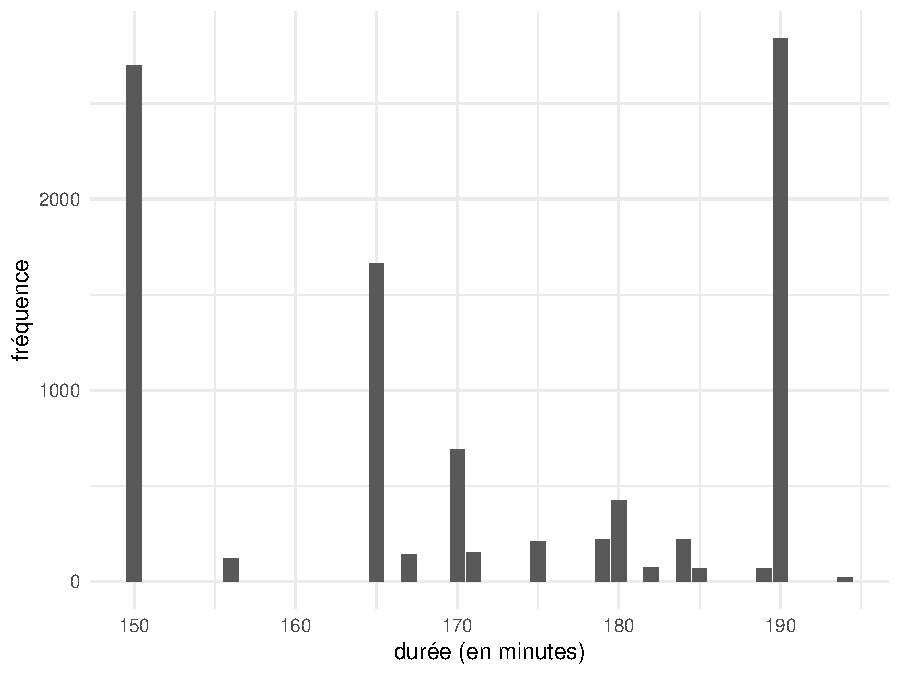
\includegraphics[width=0.7\linewidth]{MATH60604_Modelisation_statistique_files/figure-latex/renfeclt-1} 

}

\caption{Distribution empirique des temps de trajet en trains à grande vitesse.}\label{fig:renfeclt}
\end{figure}

Une analyse exploratoire indique que la durée du trajet de la base de données est celle affichée sur le billet (et non le temps réel du parcours). Ainsi, il n'y a ainsi que 15 valeurs possibles. Le temps affiché moyen pour le parcours, estimé sur la base de 9603 observations, est de 170 minutes et 41 secondes. La Figure (voir \ref{fig:renfeclt}) montre la distribution empirique des données.

Considérons maintenant des échantillons de taille \(n=10\). Dans notre premier échantillon aléatoire, la durée moyenne affichée est 170.9 minutes, elle est de 164.5 minutes dans le deuxième, de 172.3 dans le troisième, et ainsi de suite.

\begin{figure}

{\centering 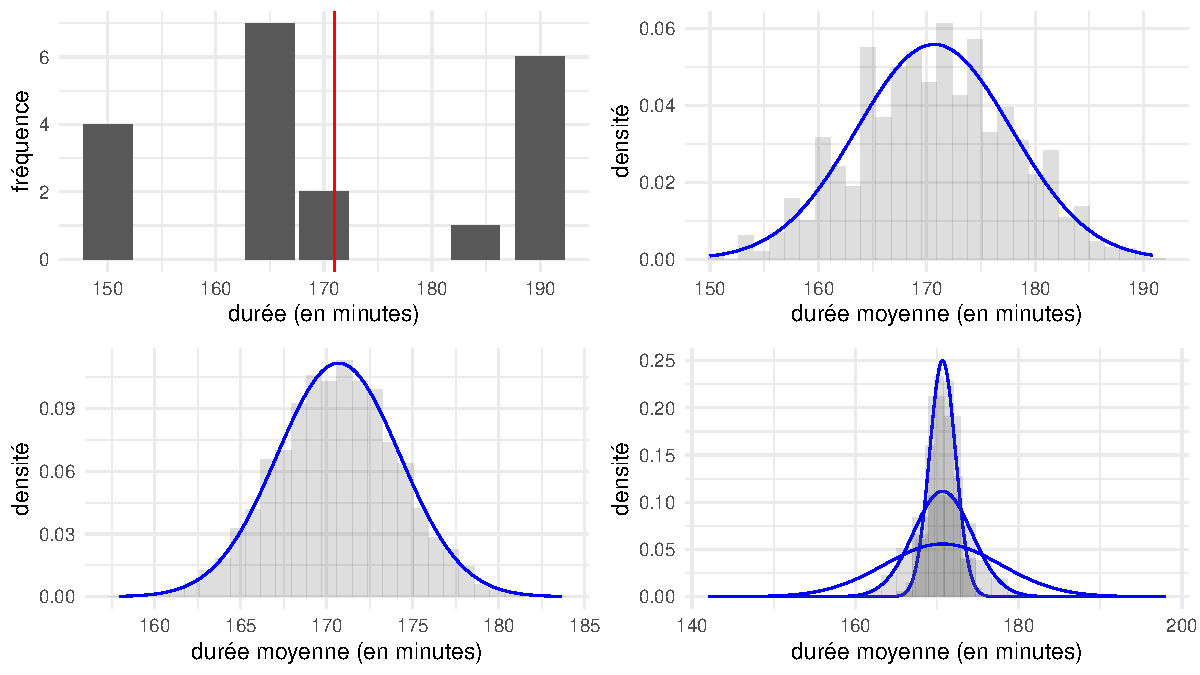
\includegraphics[width=0.9\linewidth]{MATH60604_Modelisation_statistique_files/figure-latex/renfemeanCLT-1} 

}

\caption{Représentation graphique du théorème central limite: échantillon aléatoire de 20 observations avec leur moyenne empirique (trait vertical rouge) (en haut à gauche). Les trois autres panneaux montrent les histogrammes des moyennes empiriques d'échantillons répétés de taille 5 (en haut à droite), 20 (en bas à gauche) et les histogrammes pour $n=5, 20, 100$ (en bas à droite) avec courbe de densité de l'approximation normale fournie par le théorème central limite.}\label{fig:renfemeanCLT}
\end{figure}

Supposons qu'on tire \(B=1000\) échantillons différents, chacun de taille \(n=5\), de notre ensemble, et qu'on calcule la moyenne de chacun d'entre eux. Le graphique supérieur droit \ref{fig:renfemeanCLT} montre un de ces 1000 échantillons aléatoire de taille \(n=20\) tiré de notre base de données. Les autres graphiques de la Figure \ref{fig:renfemeanCLT} illustrent l'effet de l'augmentation de la taille de l'échantillon: si l'approximation normale est approximative avec \(n=5\), la distribution des moyennes est virtuellement identique à partir de \(n=20\). Plus la moyenne est calculée à partir d'un grand échantillon (c'est-à-dire, plus \(n\) augmente), plus la qualité de l'approximation normale est meilleure et plus la courbe se concentre autour de la vraie moyenne; malgré le fait que nos données sont discrètes, la distribution des moyennes est approximativement normale.

On a considéré une seule loi aléatoire inspirée de l'exemple, mais vous pouvez vous amuser à regarder l'effet de la distribution sous-jacent et de la taille de l'échantillon nécessaire pour que l'effet du théorème central limite prenne effet: il suffit pour cela de simulant des observations d'une loi quelconque de variance finie, en utilisant par exemple cette \href{http://195.134.76.37/applets/AppletCentralLimit/Appl_CentralLimit2.html}{applette}.

Les statistiques de test qui découlent d'une moyenne centrée-réduite (ou d'une quantité équivalente pour laquelle un théorème central limite s'applique) ont souvent une loi nulle standard normale, du moins asymptotiquement (quand \(n\) est grand, typiquement \(n>30\) est suffisant). C'est ce qui garantie la validité de notre inférence!

\hypertarget{math}{%
\section{Dérivations mathématiques}\label{math}}

Cette section regroupe les dérivations mathématiques optionnelles qui sont fournies par souci de complétude.

\hypertarget{ols}{%
\subsection{Dérivation de l'estimateur des moindres carrés ordinaires}\label{ols}}

L'estimateur des moindres carrés ordinaires résoud le problème d'optimisation non-contraint
\begin{align*}
\widehat{\boldsymbol{\beta}}=\min_{\boldsymbol{\beta} \in \mathbb{R}^{p+1}}(\boldsymbol{y}-\mathbf{X}\boldsymbol{\beta})^\top(\boldsymbol{y}-\mathbf{X}\boldsymbol{\beta}).
\end{align*}
On peut calculer la dérivée première par rapport à \(\boldsymbol{\beta}\), égaler à zéro et isoler le maximum pour obtenir une formule explicite pour \(\widehat{\boldsymbol{\beta}}\),\\
\begin{align*}
\mathbf{0}_n&=\frac{\partial}{\partial\boldsymbol{\beta}}(\boldsymbol{y}-\mathbf{X}\boldsymbol{\beta})^\top(\boldsymbol{y}-\mathbf{X}\boldsymbol{\beta})\\
\\&=\frac{\partial (\boldsymbol{y}-\mathbf{X}\boldsymbol{\beta})}{\partial \boldsymbol{\beta}}\frac{\partial (\boldsymbol{y}-\mathbf{X}\boldsymbol{\beta})^\top(\boldsymbol{y}-\mathbf{X}\boldsymbol{\beta})}{\partial (\boldsymbol{y}-\mathbf{X}\boldsymbol{\beta})}\\
 \\&=\mathbf{X}^\top (\boldsymbol{y}-\mathbf{X}\boldsymbol{\beta})
\end{align*}
en utilisant la \href{http://www.stat.rice.edu/~dobelman/notes_papers/math/Matrix.Calculus.AppD.pdf}{règle de dérivation en chaîne}; on peut ainsi distribuer les termes pour obtenir l'\emph{équation normale}
\begin{align*}
 \mathbf{X}^\top \mathbf{X}\boldsymbol{\beta}&=\mathbf{X}^\top \boldsymbol{y}.
\end{align*}
Si \(\mathbf{X}\) est une matrice de rang \(p\), alors la forme quadratique \(\mathbf{X}^\top \mathbf{X}\) est inversible et l'unique solution du problème d'optimisation est celle fournie dans l'équation \eqref{eq:ols}.
\begin{align*}
\widehat{\boldsymbol{\beta}} = (\mathbf{X}^{\top} \mathbf{X})^{-1} \mathbf{X}^{\top} \boldsymbol{Y}.
\end{align*}

\hypertarget{r}{%
\section*{\texorpdfstring{\textbf{R}}{R}}\label{r}}
\addcontentsline{toc}{section}{\textbf{R}}

Je suis partisan de la \href{https://raw.githubusercontent.com/eddelbuettel/gsir-te/master/docs/Getting-Started-in-R.pdf}{philosophie Tinyverse}; voir l'introduction sur les fonctionnalités de \textbf{R} avec des ressources et des dépendances minimales.

  \bibliography{book.bib,notes60604.bib}

\end{document}
